\documentclass[bachelor,ngerman,english]{GAUBM}

\input{structure}
\input{style}
\begin{document}
	
\ThesisAuthor{Ireas Tom}{Raschke}
\PlaceOfBirth{Finsterwalde}
\ThesisTitle%
    {Untersuchung von Top-Quark Paarproduktionen mit einem Higgs Zerfall in zwei W Bosonen in einfach-leptonischen Endzuständen unter Nutzung von ATLAS}%
    {Studies of top quark pair production associated with an Higgs boson decaying into two W bosons in single-leptonic final states using ATLAS}
% \ThesisTitle{\ttHWW Rekonstruktion mit Neutrino Gewichtung \& SPA-Net}{\ttHWW event reconstruction techniques using neutrino-weighting \& SPA-Net}
\FirstReferee{Prof.~Dr.~Arnulf Quadt}
\SecondReferee{Prof.~Dr.~Ariane Frey}
\Institute{II. Physikalisches Institut}
\ReferenceNumber{XXXXXX}
\ThesisBegin{01}{04}{2024}
\ThesisEnd{30}{09}{2024}

\frontmatter
\maketitle
\cleardoublepage
\onehalfspacing
\tableofcontents
\mainmatter

% \linenumbers % for 

\chapter{Introduction}
\label{ch:introduction}
As far back as 400 BC, humans pondered about the fundamental makeup of the natural world. The earliest records of this go back to the Greek philosopher Democritus who proposed that matter cannot be infinitely divisible. Thus, there must exist the smallest, indivisible particle, which he termed the `atom' (from Greek \textit{atomos} meaning `indivisible'). Although this idea was not empirically tested but derived from philosophical thoughts, it marked the inception of the quest for a fundamental understanding of the universe.

Over the following millennia, this idea was refined by several researchers using different modern techniques. Today, research into the fundamental structure of nature continues with particle physics superseding nuclear physics. The contemporary aim of particle physics is to develop a comprehensive understanding of fundamental phenomena, centred around formulating and expanding upon the Standard Model of particle physics, which stands as the most successful description of the fundamental nature of the universe.

At the forefront of this quest for knowledge stands the Large Hadron Collider (\lhc) situated at \cern (European Organization for Nuclear Research). The \lhc, the world's most powerful particle accelerator, collides protons which reach nearly the speed of light, mimicking conditions that prevailed in the universe mere moments after the Big Bang. Through detailed analysis of these collisions, scientists aim to validate and refine the Standard Model of particle physics. 

One of the main parts at the \lhc is the \atlas experiment which takes data using a toroidally shaped particle detector around the collision beam pipe utilising cutting-edge technologies. This data is then used to study the laws of physics and to formulate models based on these observations.

The task of this analysis is to identify, separate and reconstruct the top quark pair production with an associated Higgs boson ($H$-boson) in which the $H$-boson decays into two $W$-bosons. Specifically, the single-leptonic channel is targeted. Due to its challenging topology and low cross-section, this particular channel has not been analysed independently before. Hence, a modern approach utilising techniques such as neural networks and \NW is deployed. The goal is to efficiently reconstruct the targeted events from the \atlas dataset collected in \runii and to separate them from other processes. A successful reconstruction with background separation would allow for several measurements such as the top Yukawa coupling and Higgs branching ratios using this channel. Furthermore, this study analysis the usage of neural networks and neutrino reconstruction algorithms for event reconstructions. 

This study begins by introducing the theoretical foundation of the Standard Model in Ch.~\ref{ch:standard_model}. The following Ch.~\ref{ch:experimental_setup} introduces the general experimental setup of the \lhc and the specifics of the \atlas detector. Ch.~\ref{ch:truth_matching} covers the developed truth matching algorithm used for preparing the needed training samples. The techniques applied in this project are explained in Ch.~\ref{ch:spanet} and Ch.~\ref{ch:neutrino_weighting}, which cover \spanet and \NW, respectively. The selection of events for this analysis is described in Ch.~\ref{ch:event_selection}. Ch.~\ref{ch:results} lists and explains the main results of this study. Lastly, Ch.~\ref{ch:outlook} summarises the results and discusses whether the targeted topology can be reconstructed and separated from background. Additionally, potential future tasks for further research are proposed.  



\chapter{The Standard Model of Particle Physics}
\label{ch:standard_model}
The Standard Model of particle physics (SM) \cite{theory:general_sm} stands as the most successful framework in understanding the fundamental particles and their interactions to date. It encompasses all known elementary particles along with their antiparticles, and three out of the four known fundamental forces: the strong, weak, and electromagnetic forces. Notably, gravity remains beyond the scope of the SM.


\section{Gauge Symmetry and Spontaneous Symmetry Breaking}
\label{sec:theory:gauge_symmetry_and_higgs_meachanism}
The SM is a renormalisable quantum field theory \cite{theory:quantum_fields} characterised by an internal gauge symmetry that is denoted as a SU(3)$_C$$\otimes$SU(2)$_L$$\otimes$U(1)$_Y$. A gauge symmetry is a mathematical symmetry that describes how the Lagrangian is invariant under local transformations. This means that the laws of physics do not change under these transformations. Gauge transformations form a Lie group \cite{theory:lie_groups} which necessitates the generation of an underlying gauge field \cite{theory:gauge_fields}.

%A gauge symmetry describes the fundamental principle of the invariance of physical systems under certain transformations associated with the corresponding gauge field \cite{theory:gauge_fields}. 

The SU(3)$_C$ group symmetry describes the strong interaction, stemming from quantum chromodynamics (QCD) \cite{theory:qcd_01,theory:qcd_02,theory:qcd_03,theory:qcd_04,theory:qcd_05}. It introduces colour charges and their corresponding mediators, the gluons, which are explained in more detail in Section~\ref{sec:theory:particles}.

The combined SU(2)$_L$$\otimes$U(1)$_Y$ group symmetry corresponds to the electromagnetic and to the weak force \cite{theory:qed_01,theory:qed_02,theory:qed_03,theory:qed_04,theory:qed_05}. They introduce the electrical charge $Q$ and the weak isospin $T$, respectively. Those two forces further combine at high energies on the order of $10^2$\,GeV via the electroweak unification. The latter entails the unification of the electromagnetic force \cite{theory:qed_01,theory:qed_02,theory:qed_03,theory:qed_04,theory:qed_05,theory:electroweak_01,theory:electroweak_02,theory:electroweak_03}, originating from quantum electrodynamics (QED), and the weak force, stemming from quantum flavour dynamics (QFD). The charge of the combined interaction is the weak hypercharge $Y$. However, the bosons $W^{0,1,2}$ and $B^0$ predicted by this symmetry are massless which is contradicting the massive bosons observed. This requires a process that introduces massive bosons. 

The Brout-Englert-Higgs Mechanism \cite{theory:higgs_mechanism_01,theory:higgs_mechanism_02,theory:higgs_mechanism_03} explains how bosons, and fermions as well, acquire their mass. The theory introduces a quantum Higgs-field. Every particle interacting with the field becomes massive. At very high energies, this Higgs-field is symmetric. However, at energies which we observe under normal conditions, this symmetry is spontaneously broken \cite{theory:spontaneous_symmetry_breaking}. One of the results of this is a non-zero vacuum expectation value. This vacuum energy introduces additional terms to the Lagrangian, spoiling the electroweak symmetry. These additional terms mix the four massless bosons of the theoretical electroweak symmetry ($W^1,W^2,W^3$,$B^0$) to generate the massive bosons $W^\pm, Z^0$ and the massless boson $\gamma$. The mass originates from the introduced interactions between the $W^{1,2}$ bosons and the Higgs-field. The $W$-bosons are associated with the SU(2)$_L$ symmetry group. The remaining two bosons are associated with the U(1)$_Y$ symmetry group.

Furthermore, one of the degrees of freedom introduced by the Higgs-field is not defined via the Brout-Englert-Higgs mechanism. It manifests as the scalar Higgs boson $H$ \cite{theory:higgs_mechanism_01}..


\section{Particles}
\label{sec:theory:particles}
The SM describes particles as elemental units of matter or forces. All particles have various properties such as mass, electrical charge and spin. Furthermore, each particle has an antiparticle that has the same properties as the complementary particle, but its electrical charge is inverted These antiparticles are typically denoted with a bar on top of the particle identifier. Uncharged particles do not have a complementary antiparticle. At its core, the SM categorizes particles into two main groups by their spin. These groups are fermions and bosons. In the following the focus will be on particles, since antiparticles have identical properties but with an inverted electrical charge. 


\subsection*{Fermions}
In the SM, fermions are one of the two fundamental classes of elementary particles, the other being bosons. Fermions are particles with half-integer spin. They are the basic constituents of matter and obey the Fermi-Dirac statistics as well as the Pauli exclusion principle. Moreover, Fermions can be subdivided into quarks and leptons as further described in the following sections. 

\subsubsection*{Quarks}
Quarks are elementary particles that interact via the strong nuclear force, as well as the weak and electromagnetic forces which were introduced in Section~\ref{sec:theory:gauge_symmetry_and_higgs_meachanism}. Quarks are classified into three generations. In each generation, there is an up-type and a down-type quark defined by their electrical charge and weak isospin. The up-type quarks have a positive electrical charge of +2/3 times the elementary charge $e$ and a weak isospin of +1/2. The down-type quarks have an electrical charge of -1/3 $e$ and a weak isospin of -1/2. 

For each generation, a weak isospin doublet can be defined containing two out of six quark flavours. Each quark flavour has unique properties. The first generation's doublet contains the up ($u$) and down ($d'$) quark. The second generation consists of the charm ($c$) and strange ($s'$) and the final and third generation includes the top ($t$) and bottom ($b'$) quark. %The first quark mentioned for each generation is the up-type quark while the latter is the down-type quark \cite{theory:fermions_01}.   

Note that down-type quarks denoted as $q'$ in the isospin doublets describe the weak eigenstate while $q$ describes the mass eigenstate. These two eigenstates are related via the unitary Cabibbo-Kobayashi-Maskawa (CKM) matrix \cite{theory:ckm_matrix_01,theory:ckm_matrix_02}. The matrix describes the probability amplitude $V_\text{ij}$ for the transition from quark flavour $i$ to quark flavour $j$ under the weak interaction. Furthermore, it describes the relation of the weak and mass eigenstates of down-type quarks

\begin{align}
    \begin{pmatrix}
        d'\\
        s'\\
        b'
    \end{pmatrix} &=
    \begin{bmatrix}
        V_\text{ud} & V_\text{us} & V_\text{ub}\\
        V_\text{cd} & V_\text{cs} & V_\text{cb}\\
        V_\text{td} & V_\text{ts} & V_\text{tb}
    \end{bmatrix}
    \begin{pmatrix}
        d\\
        s\\
        b
    \end{pmatrix}
    \label{eq:down-type_weak_mass_eigentstates}\,.
\end{align}

The entries in the CKM matrix are not predicted by theory. Hence, the amplitudes must be measured experimentally. The current best fitted values \cite{pdg} are the following:

\begin{align}
    \begin{bmatrix}
        V_\text{ud} & V_\text{us} & V_\text{ub}\\
        V_\text{cd} & V_\text{cs} & V_\text{cb}\\
        V_\text{td} & V_\text{ts} & V_\text{tb}
    \end{bmatrix} = 
    \begin{bmatrix}
        0.97373\pm0.00031   & 0.2243\pm0.2243   & 0.00382\pm0.00020\\
        0.221\pm0.221       & 0.975\pm0.006     & 0.0408\pm0.0014\\
        0.0086\pm0.0002     & 0.0415\pm0.0009   & 1.014\pm0.029
    \end{bmatrix}
    \label{eq:ckm_matrix}
\end{align}

With increasing quark generation, the masses of the quarks also increases. The current best measurements of the masses for the up-type quarks and the down-type mass eigenstates \cite{pdg} yield 

\begin{gather}
    \begin{aligned}
        m_u &= 2.16^{+0.49}_{-0.26}\,\text{MeV},    & m_d &= 24.68^{+0.48}_{-0.17}\,\text{MeV},\\
        m_c &= 1.27^{+0.02}_{-0.02}\,\text{GeV},    & m_s &= 93.4^{+8.6}_{-3.4}\,\text{MeV},\\
        m_t &= 172.69^{+0.30}_{-0.30}\,\text{GeV},  & m_b &= 4.18^{+0.03}_{-0.02}\,\text{GeV}.
        \label{eq:mass_quarks}
    \end{aligned}
\end{gather}

Quarks also carry a property known as colour charge \cite{theory:qcd_01,theory:qcd_02}. It is analogous to the electric charge but associated with the strong nuclear force. However, unlike electric charge, which comes in positive and negative values, colour has six possible states: red, green, blue and their complements anti-red, anti-green, and anti-blue. Quarks always combine to a state in which all three colours are combined, or any colour combined with its complement \cite{theory:qcd_02}. These states are called colourless. This is known as colour confinement and is responsible for the fact that isolated quarks are never observed in nature.

\subsubsection*{The Top Quark}
The top quark will be explained in more detail since its of particular interest for this project. The discovery of the top quark took place in 1995 at \fermilab through the efforts of the \dzero \cite{theory:top_discovery_01} and \cdf \cite{theory:top_discovery_02} experiments that both discovered the top quark independently. The top quark is acknowledged as the most massive among all quarks. Producing \tquarks needs significant energies owing to high mass of the \tquark. Such energies are attainable in hadron colliders. The top quark decays before it hadronises due to its brief lifetime is approximately $\tau_t\approx5\cdot10^{-25}\,\text{s}$ \cite{pdg}. It decays into a $W$-boson and a down-type quark which then undergoes hadronisation. 

The likelihood of decaying into a specific down-type quark is determined by the previously mentioned CKM matrix in Equation~\ref{eq:ckm_matrix}. Comparing the values of $V_\text{td}$ and $V_\text{ts}$ to $V_\text{tb}$ from Equation~\ref{eq:ckm_matrix} shows the predominant top decay mode to $b$ quarks.
 
The $W$-boson, the second particle from the top decay, also decays further. As explained later, it can decay either into a charged lepton \& neutrino pair or into a quark and antiquark pair. Thus, the resulting final state from a top decay include one quark and a lepton or three quark, depending on the $W$-boson decay mode. 

\subsubsection*{$b$ tagging}
To precisely identify $t$ quarks, an accurate algorithm to distinguish $b$ is necessary. The reason for this is the top quarks predominant decay mode into $b$ quarks which was explained previously. To achieve this, $b$ tagging is introduced \cite{btag:atlas,btag:cms}.

The accurate identification of works by exploiting the properties of the $b$ quark. It has a relatively large mass and a long lifetime. The latter is explained by its suppressed decay modes. Equations~\ref{eq:ckm_matrix} shows that the $V_{tb}$ element is the highest values for $b$ quark row. Thus, the $b$ flavour couples predominantly to the $t$ flavour and decay modes into other flavours are suppressed. However, the $t$ is significantly heavier than the $b$ quark as seen in Equation~\ref{eq:mass_quarks}. Hence, the decay into a top quark is also strongly suppressed.

Due to the long lifetime of the $b$ quark, it can travel a measurable distance before decaying. Thus, its decay products do not originate from the primary vertex of the collision. Instead, reconstructing these decay products yields a displaced vertex position which is typically referred as `secondary vertex'. This reconstruction combined with the hard momentum spectra of the $b$ quarks decay products yields a sufficiently accurate $b$ tagging which reaches an efficiency of 70\% \cite{btag:performance} at the \atlas experiment. This approach can also be applied, to a lesser extent, to charm tagging. 


\subsubsection*{Leptons}
Leptons are the second group of fermions. They do not experience the strong nuclear force and interact via the weak and electromagnetic forces. Analogue to the quarks, there are three generations of leptons: electron, muon and tau \cite{theory:general_sm}. These are typically denoted as $e$, $\mu$ and $\tau$, respectively.

Each generation consists of a weak isospin doublet containing an uncharged neutrino $\nu_l$ and its respective charged lepton $l$ \cite{theory:general_sm}. Charged leptons have an electrical charge of -1$e$ and a weak isospin of -1/2. Furthermore, the charged leptons are massive. Their masses increase with higher generations as current measurements \cite{pdg} show

\begin{gather}
    \begin{aligned}
        m_e     &=0.511\pm0.001\,\text{MeV},\\
        m_\mu   &=105.66\pm0.001\,\text{MeV},\\
        m_\tau  &=1776.86\pm0.12\,\text{MeV}.
        \label{eq:mass_leptons}
    \end{aligned}
\end{gather}

On the contrary, the uncharged neutrinos have no electrical charge \cite{pdg}, a weak isospin of +1/2 and are predicted to be massless by the SM \cite{theory:general_sm}. However, the later prediction is conflicting with some observed phenomena that are explained in Section~\ref{sec:theory:bsm}.


\subsection*{Bosons}
Bosons are the second group of particles in the SM. Unlike the Fermions, bosons have integer values of spin and obey Bose-Einstein statistics. Bosons can be subdivided into gauge bosons that mediate three of the four fundamental forces and the Higgs boson. %They do not obey the Pauli exclusion principle and thus, multiple bosons can occupy the same quantum state simultaneously \cite{theory:fermions_bosons}.

\subsubsection*{Gauge Bosons}
In the SM there are 4 different gauge bosons types \cite{theory:general_sm} that are responsible for the interaction between particles of the SM. While many of their properties differ, they all have spin 1. The remaining properties are discussed in the following paragraphs.  

The photon ($\gamma$) is the massless mediator of the electromagnetic force \cite{theory:qed_02,theory:qed_04,theory:qed_05}. It itself is not electrical charged and thus, couples to positively and negatively charged particles equally. The behaviour of photons is determined by QED which was introduced in Section~\ref{sec:theory:gauge_symmetry_and_higgs_meachanism}.

A gluon ($g$) is a type of massless gauge bosons that is responsible for the mediation of the strong nuclear force \cite{theory:qcd_01}. They couple to the colour charge of quarks. And unlike the photon, gluons themselves also carry colour charges which are exchange during a strong interaction. There are eight different possible colour combination for gluons due to the rules of QCD. Since they carry the charge they couple to, gluons are able to couple to other gluons. These processes are called self-couplings.

Lastly, there are $W^\pm$- and $Z^0$-bosons. These are the mediators of the weak nuclear force. In contrast to the other gauge bosons, these are massive due to symmetry breaking in the Brout-Englert-Higgs Mechanism which is explained in more detail in Section~\ref{sec:theory:gauge_symmetry_and_higgs_meachanism}. Their masses were measured to be \cite{pdg}

\begin{gather}
    \begin{aligned}
        m_W &= 80.377\pm0.012\,\text{GeV},\\
        m_Z &= 91.1876\pm0.0021\,\text{GeV}. 
        \label{eq:mass_wz}
    \end{aligned}
\end{gather}

$W^\pm$-bosons have an electrical charge of $\pm1e$. Moreover, they have a weak isospin. Its third component of the weak isospin is $\pm1$, respectively. Fermions interacting with the $W$-bosons undergo a flavour transition. Charged leptons convert to lepton neutrinos and vice versa. Quarks also change their flavour. Their transition rate from one quark to the other is determined by the previously discussed CKM matrix. Couplings with the $W$-bosons are CP violating. The $Z^0$-boson, as indicated by its superscript, has no electrical charge and its third component of the weak isospin is 0. 

\subsubsection*{Higgs Boson}
The Higgs boson ($H^0$) was the last particle of the SM discovered in 2012 by the combined efforts of the \atlas \cite{theory:higgs_discovery_01} and \cms \cite{theory:higgs_discovery_02} experiments. The Higgs boson's detection gave strong support to the Brout-Englert-Higgs mechanism discussed in Section~\ref{sec:theory:gauge_symmetry_and_higgs_meachanism}. It is electrically neutral and has spin 0, making it the only scalar boson. Moreover, it is the second-heaviest particle ever detected with current measurements \cite{pdg} showing a mass of 

\begin{gather}
    \begin{aligned}
        m_H=125.25\pm0.17\,\text{GeV}.
        \label{eq:mass_h}
    \end{aligned}
\end{gather}

Furthermore, it represents the quantum manifestation of the Higgs field and thus, couples to mass of particles. Its production and decay branching ratios are strongly dependent on the mass of the interacting particle. The higher the mass, the stronger is the Higgs coupling resulting in higher branching ratios. The reason for this is the linearity between the Yukawa coupling strength and the (fermion) masses. Hence, the most common production modes are in combination with either $t$ quarks or $W$-/$Z$-bosons. 

For the decay, the most likely modes are decays into pairs of $b$ quarks or $W$- and $Z$-bosons. While the Higgs coupling of the $t$ is stronger than the $b$, the decay into a $t$ quark pair is strongly suppressed, due to its significantly higher mass $2m_t>m_H$. Couplings with the Higgs field (thus also with the $H$-boson) are described as Yukawa couplings that also generate the mass of fermions and bosons \cite{theory:higgs_mechanism_01,theory:higgs_mechanism_03}. Since the $H$-boson is massive, it can couple to itself, similar to the gluon. This gives rise to Higgs self-coupling.   

\section{Beyond the Standard Model}
\label{sec:theory:bsm}
Despite the incredible range of phenomena that the SM can predict and explain for example the existance and properties of the $W$-, $Z$- and $H$-bosons as well as its precision, certain phenomena contradict its fundamental explanations. 

\subsubsection*{Neutrino Oscillation}
One of these problematic observations is neutrino oscillation \cite{bsm_neutrino_oscillation_01,bsm_neutrino_oscillation_03}. It describes how neutrinos change their flavour while propagating through space. The first indication was found by the Homestake Experiment in 1968 \cite{bsm_neutrino_oscillation_04}. It detected solar neutrinos using a large tank of fluid and observed a neutrino deficit. In 1998, the Super-Kamiokande experiment studied atmospheric neutrinos and discovered a changing electron/muon neutrinos flux during the runtime \cite{bsm_neutrino_oscillation_02}. 

The oscillation originates from the separation of the flavour eigenstates of the neutrinos ($\nu_e$, $\nu_\mu$, $\nu_\tau$) and its mass eigenstates ($\nu_1$, $\nu_2$, $\nu_3$). If these eigenstates are not equal, then neutrinos could change their flavour. The probability of a neutrino of a given flavour transitioning into another flavour depends on the mixing angles and mass differences between the mass eigenstates. The observed oscillation necessitates at least two massive neutrinos. Contradictory, the SM predicts all neutrinos as massless which would result in their flavour and mass eigenstates to be identical. Consequently, the oscillation would be prohibited and thus, the SM fails to account for neutrino oscillations. 

\subsubsection*{Gravity}
Another obvious problem with the SM is the absence of gravity. While the force of gravity is observed, the SM has no boson responsible for mediating gravity. Possible solutions include the introduction of a hypothetical massless and uncharged graviton \cite{bsm_gravity_01} or string theory \cite{bsm_gravity_02}. Without an explanation of gravity, the SM can not achieve to be a unified theory of everything. 

\subsubsection*{Further Contradictions}
There are more contradicting observations that need explanations beyond the SM. These examples contain, but are not limited to, dark matter \cite{bsm_dark_matter_01,bsm_dark_matter_02,bsm_dark_matter_03}, atype of invisible mass needed for stellar observations, prediction of vacuum energy \cite{bsm_vacuum_energy}, a deviation between QFT and cosmological predictions and the hierarchy problem \cite{bsm_hierarchy}, a relatively low $H$-boson mass that necessitates fine-tuning. For each of the problems, severalBSM explanations such as supersymmetry \cite{bsm_supersymmetry} or modified gravity \cite{bsm_mond} are possible.


\section{Higgs-Associated Top Quark Pair Production}
\label{sec:theory:tthww}
The targeted event topology is the $H$-boson associated top quark pair production in which the $H$-boson decays into two $W$-bosons. It consists of a fully hadronic decaying \ttbar pair with an additional $H$-boson. The latter decays into two $W$-bosons which then further decay semi-leptonically, which means that one $W$-boson decays hadronically into two quarks while the other decays leptonically into a lepton neutrino pair. In the following, these events will be referred to as semileptonic \ttHWW events. The corresponding Feynman diagram of the targeted topology can be seen in Figure~\ref{fig:feynman_tthww}. 

\begin{figure}[t]
    \centering
    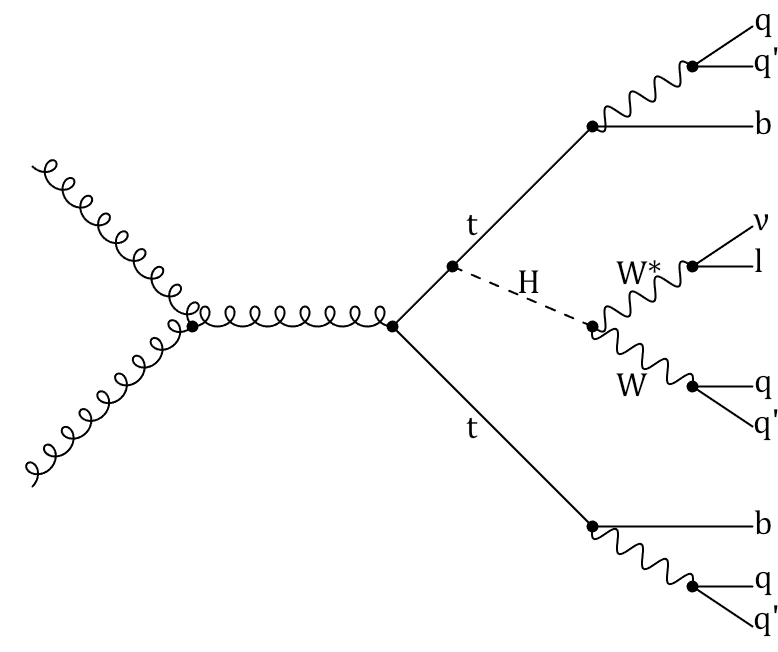
\includegraphics[width=.6\textwidth]{figures/feynman/feynman_labeled2.png}
    \caption{Feynman diagram of the targeted \ttHWW event topology.}
    \label{fig:feynman_tthww}
\end{figure}

The rarity of the semileptonic \ttHWW events makes its measurement difficult. Fig.~\ref{fig:theory:total_crosssections} depicts a summary of several event cross-section measured by \atlas. It shows the dominating \ttbar background with significantly higher a cross-section of ($834\pm47$)\,pb \cite{ttbar_cross_section_theoretical} compared to \ttH which reaches ($507\pm61$)\,fb \cite{higgs_cross_section_theoretical}. These theoretical cross-section refers to all $t$ quark and $H$-boson decay modes. Hence, the \ttH events are three orders of magnitude rarer than \ttbar events. Other background processes such as $tW$, \ttZ and \ttW have cross-sections higher or close to \ttH.

However, this study focuses on a particular $H$-boson decay mode. Hence, the branching ratio of the Higgs decay must be taken into account. For the previously stated SM $H$-boson mass $M_H$, the theoretical branching ratio of $H\rightarrow WW$ is the second highest at ($21.5\pm1.0$)\,\% \cite{yellow_report_4_higgs}. Furthermore, the $W$-boson decay ratios are ($67.41\pm0.27$)\,\% hadronically and ($32.58\pm0.47$)\,\% leptonically \cite{pdg}. Multiplying the \ttH cross-section with these decay ratios and taking the $W$-permutations into account yields a final cross-section of ($56.8\pm12.3$)\,fb for the targeted semileptonic \ttHWW event topology. This results in more than 10000 expected \ttbar events per semileptonic \ttHWW event. Taking other background processes into account, semileptonic \ttHWW events become even more difficult to measure.

To reduce some of the backgrounds, the semileptonic decay mode is chosen. The implemented single lepton limitation helps suppressing $W$+jets and QCD multijet backgrounds. 

In the targeted topology, the $H$-boson production is expected to be a resonance process. Hence, only on-shell $H$-boson masses are considered. Due to the insufficient mass of the $H$-boson to create two on-shell $W$-bosons, one of the two $W$-bosons must be off-shell. This is denoted by the asterisk superscript $W^*$. The analysis restricts to events where the on-shell $W$-boson is decaying hadronically. This simplifies the event reconstruction since the invariant mass of the two selected decay jets should match the SM $W$-boson mass $M_W$ as close as possible. Thus, it can be used to suppress some of the main backgrounds due to the constraint on the decay jet properties. However, it also necessitates that the off-shell $W^*$-boson decays leptonically which complicates the leptonic reconstruction.

\begin{figure}[t]
    \centering
    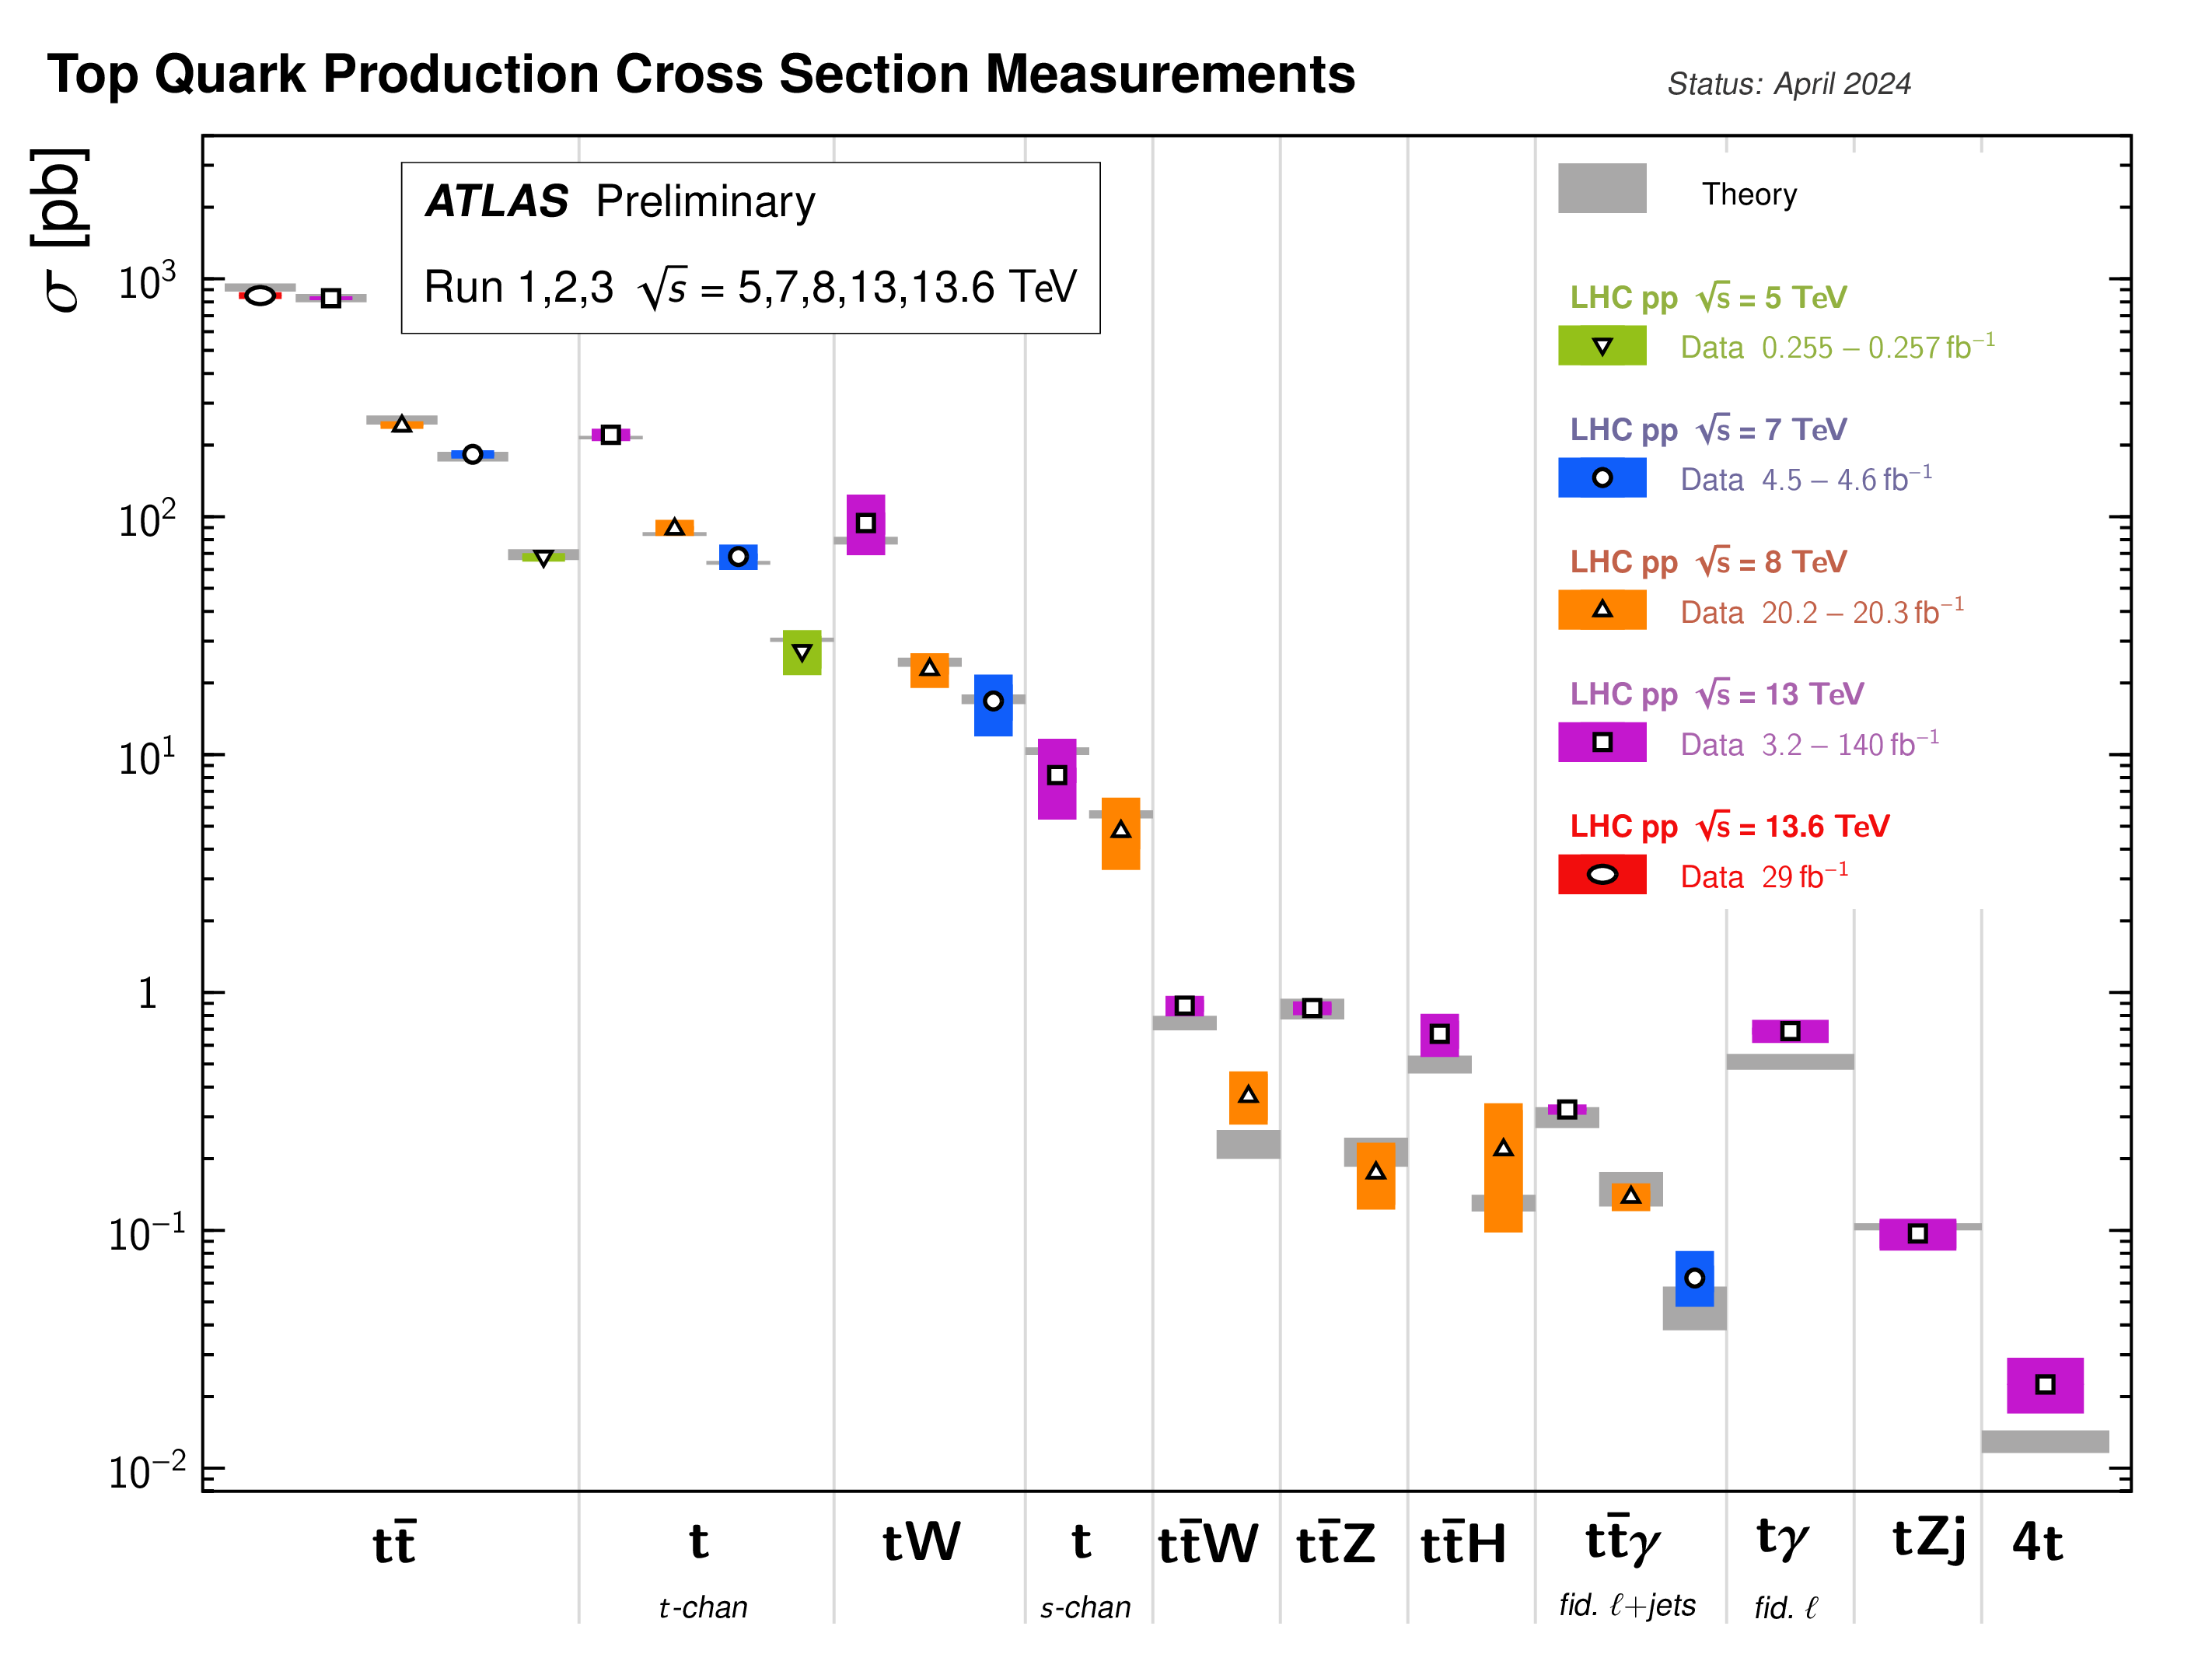
\includegraphics[width=.95\textwidth]{figures/cross_section/top_total_cross_sections.png}
    \caption{Overview of several $t$ quark related production cross-section measurements with theoretical predictions calculated at next to leading order or higher \cite{theory:cross_sections}.}
    \label{fig:theory:total_crosssections}
\end{figure}


% This channel offers insight into the spin coupling between the spin-0 $H$-boson and its to decay spin-1 $W$-bosons as discussed in Section~\ref{sec:theory:bosons}. Furthermore, additional measurements on the top Yukawa $tH$ coupling \cite{theory:why_tH_coupling} or Higgs decay branching ratios are possible using this channel. However, due to the targeted Higgs decay mode, the missing energy due to the $\nu$ in the final state as well as the off-shell $W^*$-boson pose a challenge for the event reconstruction. 


\chapter{Experimental Setup}
\label{ch:experimental_setup}
To collect data on \ttHWW events, a high-energy particle collider is necessary. Additionally, a setup for signal detection and suitable reconstruction algorithms are required. This chapter introduces the Large Hadron Collider \cite{lhc_01,lhc_02} in Section~\ref{sec:exp:lhc} which is used for collecting the data for this project. It is one of the most important particle accelerators worldwide and includes many experiments such as the \atlas experiment \cite{atlas}. The \atlas experiment provides the data for the project and is discussed in great detail in Section~\ref{sec:exp:atlas}. Other experiments are briefly described in Section~\ref{sec:exp:other_experiments}.

\section{Large Hadron Collider}
\label{sec:exp:lhc}
The Large Hadron Collider (\lhc) \cite{lhc_01,lhc_02} is the world's largest and most powerful particle accelerator. It's located underground near Geneva, Switzerland, crossing the border between Switzerland and France. Specifically, it's situated at the European Organization for Nuclear Research (\cern). The collider spans 27\,km in circumference and reaches depths of up to 175\,m. Along the collider, there are several detectors build which will be explored in Section~\ref{sec:exp:atlas} and Section~\ref{sec:exp:other_experiments}. Figure~\ref{fig:lhc_aerial_view} shows and aerial view of the regions above the \lhc demonstrating its size and showing the position of the different experiments.

It is used to create and accelerate bunches of protons close to the speed of light. Then a collision of these bunches is induced. During such a collision, partons from the protons interact and give rise to a large multitude of processes. By studying the debris produced by these collisions, physicists can gain insights into fundamental questions about the nature of the universe. Moreover, predictions of the SM introduced in Chapter~\ref{ch:standard_model} can be tested with such collisions. 

\begin{figure}[t]
    \centering
    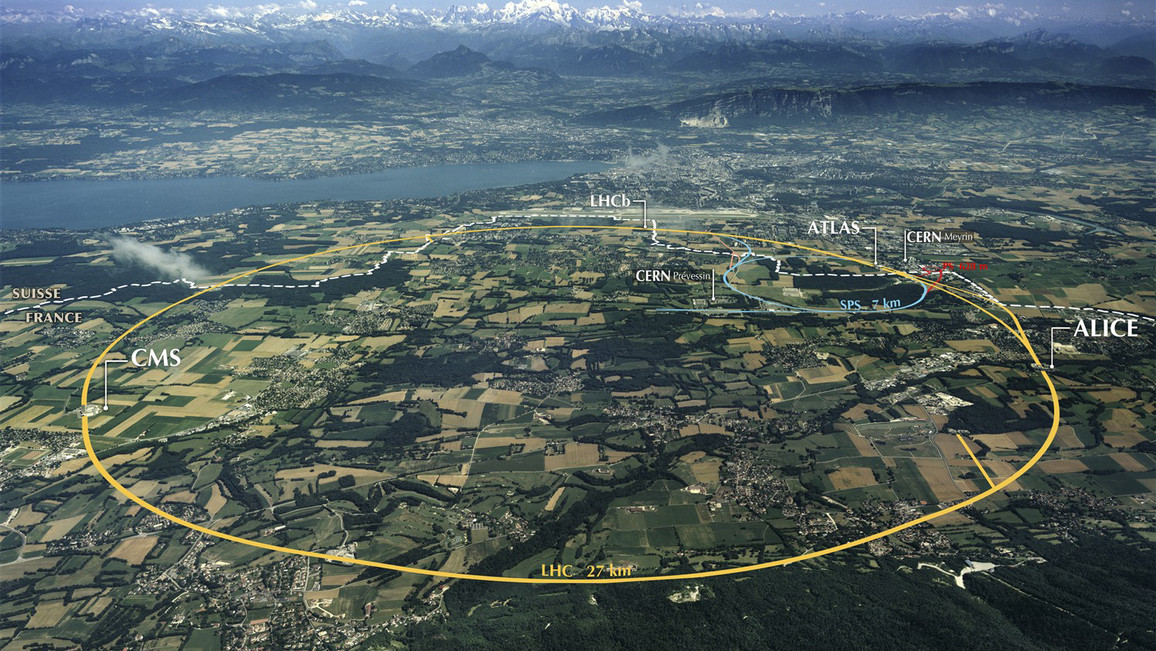
\includegraphics[width=.80\textwidth]{figures/lhc/lhc_overview.jpg}
    \caption{Aerial view above the Large Hadron Collider showing its size. The different experiments are marked along the \lhc course. \copyright{} \cern, Maximilien Brice}
    \label{fig:lhc_aerial_view}
\end{figure}

The \lhc is operating for certain time periods with long shutdowns in between. The first operation period, \runi, was active from November 2009 until February 2013. It started with a beam energy of 1.2\,TeV which was then later increased to 3.5\,TeV. In the last year it reached a beam energy of 4\,TeV. During the operation, 5.6\,fb$^{-1}$ had been accumulated by \atlas and \cms. Then Long Shutdown 1 followed \runi. 

In April 2015, \runii started. The second run reached beam energies of 6.5\,TeV and lasted until December 2018. It acquired an integrated production of 160\,fb$^{-1}$. The Long Shutdown 2 then held on until 2022. 

The currently active \runiii launched in April 2022 with a centre-of-mass energy of 13.6 TeV, 6.8 TeV per beam. It is planned to operate until the coming Long Shutdown 3 planned for 2026. 


\section{The ATLAS Experiment}
\label{sec:exp:atlas}
\atlas (A Toroidial \lhc ApparatuS) \cite{atlas} is one of the four main experiments at the \lhc. Its detector is designed as a general-purpose detector to explore a wide range of physics phenomena \cite{atlas:tech_design_report_01,atlas:tech_design_report_02}. The detector began its operation along the start-up of the \lhc. It spans a height of 25\,m and a length of 44\,m. It is build almost hermetically around the \lhc beam pipe as a toroidal shape which can be seen in Figure~\ref{fig:atlas_overview}. Constructing the detector so close to the interaction point allows measuring the maximum possible phase space. The coordinate system used in \atlas is important for understanding the detector and is introduced in Section~\ref{sec:exp:atlas_coordinate_system}. Within the detector, there are several layers that are explained in great detail in Section~\ref{sec:exp:atlas_detector}.

\begin{figure}[t]
    \centering
    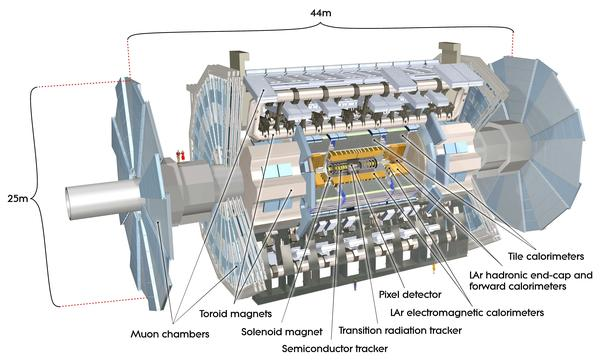
\includegraphics[width=.75\textwidth]{figures/lhc/atlas_overview.jpg}
    \caption{Overview of the \atlas detector showing its size and structure. Moreover, every important component is labelled. \copyright{\cern}}
    \label{fig:atlas_overview}
\end{figure}


\subsection*{Coordinate System for ATLAS}
\label{sec:exp:atlas_coordinate_system}
The \atlas detector is built as a cylinder. Thus, a fitting coordinate system must be defined. Every position in the detector is defined by the $z$ position parallel to the beam axis, the azimuth angle $\phi$ along the detector and the pseudo-rapidity $\eta$ with respect to the collision point of the detector. The latter quantity $\eta$ is defined by 

\begin{align}
    \eta = -\text{ln}\left(\text{tan}\frac{\theta}{2}\right)
\end{align}

with $\theta$ the polar angle. Figure~\ref{fig:atlas_coordinate_system} illustrates a 2 dimensional projection of the cylinder at a fixed distance from the centre. 

\begin{figure}[t]
    \centering
    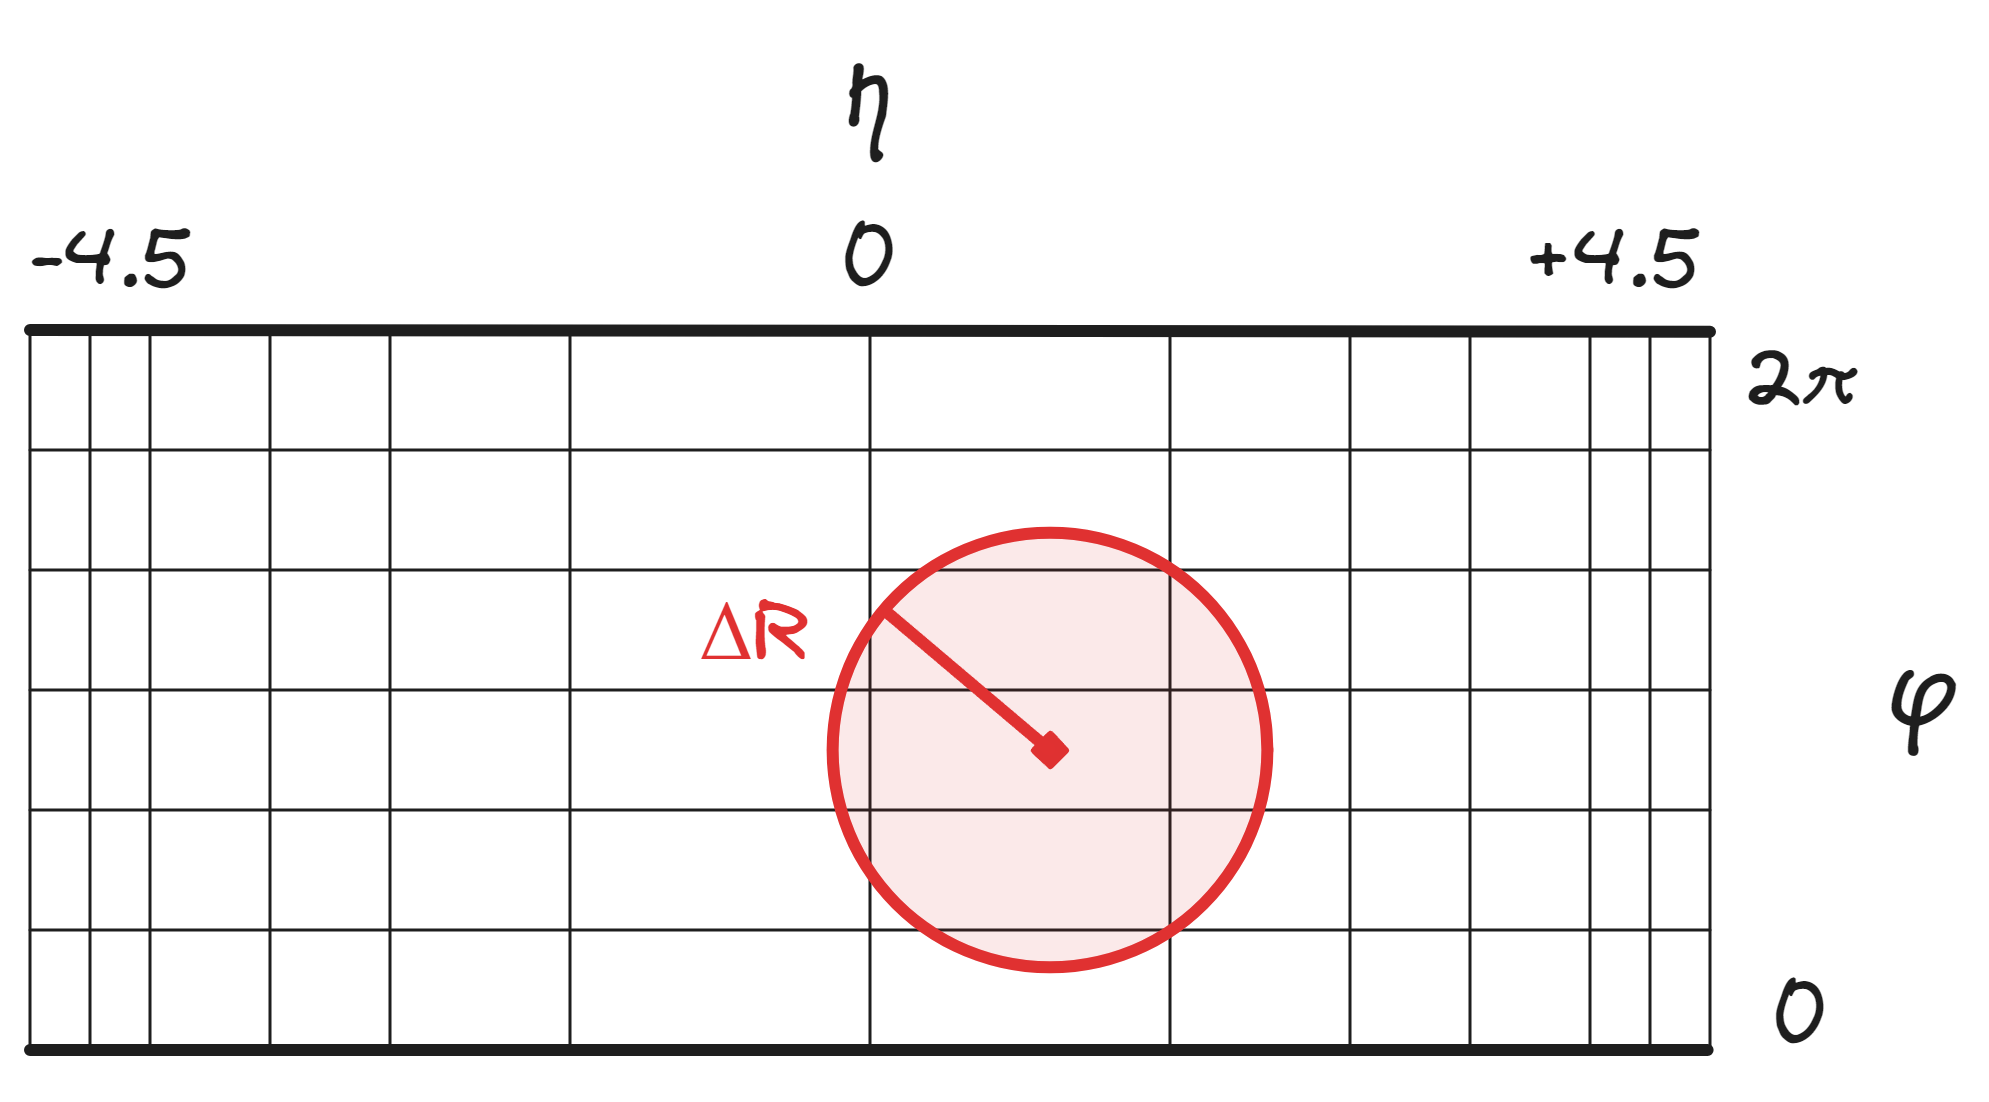
\includegraphics[width=.72\textwidth]{figures/lhc/atlas_coordinate_system.excalidraw.png}
    \caption{Sketch visualising the \atlas coordinate system using the azimuth angle $\phi$ and pseudo-rapidity $\eta$. It represents the rolled out detector cylinder. Moreover, it shows how a spatial cone defined by $\Delta R$ would look like.}
    \label{fig:atlas_coordinate_system}
\end{figure}

To properly work with spatial separations in this coordinate system, the variable

\begin{align}
    \Delta R &= \sqrt{\left(\Delta \phi\right)^2 + \left(\Delta \eta\right)^2}\label{eq:delta_r}
\end{align} 

is introduced. It represents a cone around each point in the coordinate system as shown in Figure~\ref{fig:atlas_coordinate_system}. This should not be confused with $R$ which is typically the radius from the beam pipe. Hence, expressions such as $R\phi$ correspond to the radial scaled azimuth angle and is used in classifying detector resolutions as seen before.


\subsection{Components of the ATLAS Detector}
\label{sec:exp:atlas_detector}
The detector of the \atlas experiment is of particular interest for this project. The following sections will cover its elements including the detector modules and magnetic systems in great detail. An overview of the detector is shown in Figure~\ref{fig:atlas_overview}. The individual layers of the detector are further visualised in Figure~\ref{fig:atlas_layers}. 

\begin{figure}[t]
    \centering
    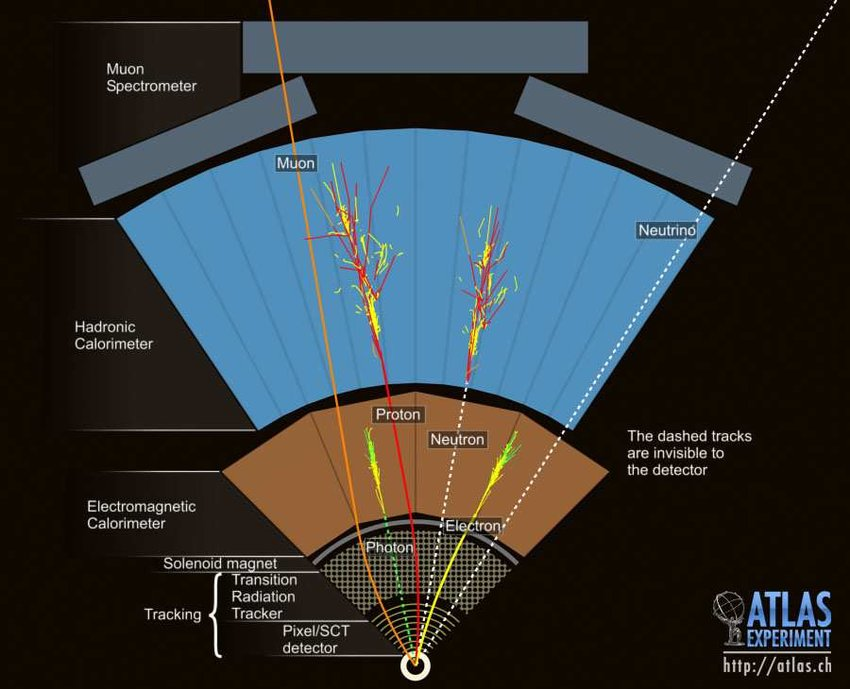
\includegraphics[width=.70\textwidth]{figures/lhc/atlas_layers.png}
    \caption{Cross-section of the concentric layers within the \atlas detector. \copyright{\cern}}
    \label{fig:atlas_layers}
\end{figure}

\subsubsection*{Magnetic System}
For the measurement of particle trajectories and their curvature, significant magnetic fields are required. For that reason, \atlas implemented superconducting magnet system build from Aluminium, Copper and Niobium-Titanium alloy. 

It includes a central solenoid magnet surrounding the Inner Detector. It provides a central field of 2\,T \cite{atlas:tech_design_report_01}. Since the central solenoid is placed right before the calorimeter, this magnet is build as thin as possible. 

Furthermore, three large air-core toroids generate an additional magnetic field for the outer muon spectrometer. Each consisting of eight symmetrical coils placed radially around the beam axis \cite{atlas:tech_design_report_01}. These magnet systems are cooled using liquid Helium at 4.5\,K \cite{atlas:tech_design_report_01}. 

\subsubsection*{The Inner Detector}
The Inner Detector \cite{atlas:tech_design_report_inner_01,atlas:tech_design_report_inner_02} is a combined system of high-resolution detectors close to the beam pipe and continuous tracking elements at outer radii. Its task is to measure the particles' momentum. As mention before, the complete Inner Detector is surrounded by the 2\,T central solenoid magnet. Charged particles are deflected inside the detector, due to the Lorentz force. By precisely measuring the curvature, momentum measurements and particle track reconstruction are achieved.

Its detector modules are placed either in the barrel or the end-cap region. The first region is arranged on concentric cylinders surrounding the beam axis and typically covers the low $\eta$ region. The later regions detectors are installed on disks perpendicular to the beam axis and cover the remaining space for a full coverage up to $\eta\pm2.5$.

The innermost detector tiles are semiconductor pixel detectors \cite{atlas:tech_design_report_01,atlas:pixel_detector}. The first barrel layer is only 4\,cm from the beam pipe, covers an area of 0.2\,m$^2$ and measures the complete space up to $\eta=\pm2.5$. It reaches a resolution of $\sigma_{R\phi}=12\,\upmu\text{m}$ and $\sigma_{z}=66\,\upmu\text{m}$. This layer is followed by two more barrel layers that cover $\eta=\pm1.7$ and reach the same resolution. To compensate this lower $\eta$ acceptance, 5 end-cap disks are placed in each side. These cover the remaining space up to $\eta=\pm2.5$. Each module is only 21.4\,mm wide and 62.4\,mm long containing 61440 pixels controlled by 16 chips. Every pixel detector has its individual circuit including buffering to store data until the trigger decision. While the precision and radiation resistance of these pixel detectors are remarkable, they also introduce some material before the calorimeters and are expensive. Hence, the amount of pixel detectors that can be included in the detector is limited. 

Directly surrounding the pixel modules, the silicon strips are introduced \cite{atlas:tech_design_report_01,atlas:strip_detector}. It is subdivided into four barrel layers for the $\eta$-range up to $\eta=\pm1.4$ and 9 end-cap wheels on each side for the remaining space up to $\eta=\pm2.5$. Compared to the pixel modules, they achieve a slightly lower precision of $\sigma_{R\phi}=16\,\upmu\text{m}$ and $\sigma_{z/R}=580\,\upmu\text{m}$. Each detector is 6.28x6.40\,cm$^2$ in size and includes 768 strips. Moreover, each module consists of four of these silicon detectors.

Straw tube trackers around the previous modules allow for a lot of measured tracking points \cite{atlas:tech_design_report_01,atlas:transition_detector}. In the barrel regions, these are placed parallel to the beam axis. In contrast to the end-caps where these are aligned perpendicular to the beam axis. Previously, these were filled with a Xenon gas mixture. However, due some leakage this Xenon was changed to Argon to reduce costs. While these achieve significantly worse resolutions of $\sigma=170\,\upmu\text{m}$, they can cover a greater area at lower cost and less material per tracking point. Hence, they strongly contribute the precise momentum measurements.

\subsubsection*{The Calorimeters}
The calorimeters \cite{atlas:tech_design_report_01,atlas:calorimeter} are used to detect charged particles by absorbing them, allowing for a measurement of their deposited energy. The physical process of showering which allow such measurements was previously described in Chapter~\ref{ch:standard_model}. \atlas' calorimeter system is subdivided into four parts: electromagnetic calorimeter, hadronic barrel calorimeter, hadronic end-cap calorimeter and hadronic forward calorimeter.

The first of these calorimeters, the electromagnetic calorimeter \cite{atlas:tech_design_report_01}, is built from lead, liquid argon and kapton electrodes. It covers the pseudorapidity range up to $\eta=\pm3.2$ while the barrel region can detect up to $\eta=\pm1.475$. It is the innermost calorimeter and is primarily responsible for detecting photons and electrons. 

The hadronic calorimeter \cite{atlas:tech_design_report_01} is build around the electromagnetic calorimeter and is build from plastic scintillator plates and iron absorber in the barrel region and from copper, lead and liquid argon in the end-cap regions. This separation is done to optimise the detector for the varying requirements of the great $\eta$ range. The barrel region reaches up to $\eta=\pm1.7$ and the end-caps up to $\eta=\pm3.2$. Its thickness is one of the most important parameters for the calorimeter, since it has to contain the hadronic showers and thus, minimise punch-trough into the adjacent Muon Spectrometer.

The forward hadronic calorimeter \cite{atlas:tech_design_report_01} is implemented to cover the strongly boosted region of $3.1<|\eta|=4.9$. It as well is build from a lead liquid argon mixture with additional electrodes from copper or a tungsten alloy.

\subsubsection*{The Muon Spectrometer}
The outermost measurement part of the \atlas detector is the Muon Spectrometer \cite{atlas:tech_design_report_01,atlas:muon_chamber}. It bends the muon tracks by utilising the previously explained air-core magnets. The magnetic field is mostly orthogonal to the muon trajectories. In the region up to $\eta=\pm1.0$ the large barrel toroid magnet provides the needed magnetic field. Within the acceptance range of $1.4\leq|\eta|\leq2.7$ two smaller end-cap magnets bend the tracks. Between of these regions is the transition region where the deflection of the muon trajectories is done by the magnet field of both magnetic systems. The muon spectrometer consists of four parts.

The first part is the monitored drift tube chamber which make up 800\,m$^3$ in volume. It consists of 30\,mm diameter aluminium tubes operating with a mixture of 93\% argon and 7\% CO$_2$. The single-wire resolution is $\sim$80\,$\upmu$m. To increase the overall resolution, multi-layer pairs of multiple tubes are utilised.

The New Small Wheel project replaced the original Cathode Strip Chambers \cite{atlas:muon_chamber,atlas:muon_chamber_upgrade,atlas:new_small_wheel}. It was installed after \runii and uses Micro-Mesh Gaseous Structure as well as small-strip thing gab chambers. The former being a detector consisting of a planar electrode and a thin steel mesh forming a drift chamber. It is filled with the same argon-CO$_2$ mixture as the first drift tube chamber. Its spatial resolution reaches 73\,$\upmu$m. The later thing gab chambers consist of a gold-plated tungsten wire grid placed between two electrodes. The electrodes are made from a carbon-epoxy mixture. The detector module reaches a spatial resolution of 100\,$\upmu$m at the rate of up to 20\,kHz/cm$^2$.

The resistive plate chambers \cite{atlas:tech_design_report_01,atlas:muon_chamber,atlas:muon_chamber_upgrade} are another gaseous detector. It uses a non-flammable C$_2$H$_2$F$_4$ SF$_6$ gas mixture. Again, the electrodes of the detection chamber are made from carbon. The panels themselves are made polystyrene placed between aluminium sheets. They achieve a spatial resolution of 1\,cm and a temporal resolution of 1\,ns.

The thin gab chambers \cite{atlas:tech_design_report_01,atlas:muon_chamber} are the last chamber of the muon spectrometer. It is a proportional chamber using a flammable gas mixture of 55\% CO$_2$ and 45\% n-pentane. Even though it needs additional safety precautions, it is less sensitive to mechanical deformations, yields nearly Gaussian pulse height distributions and has a small dependence on the incident angle. The distance of both electrodes are 2.8\,mm.

\subsubsection*{Trigger System}
The aforementioned detector systems are able to detect and record significant amounts of data. The initial bunch-crossing rate of up to 40\,MHz result in an interaction rate of $\sim$1\,GHz \cite{atlas:tech_design_report_01} which is too much to save. Approximately only 0.1\,kHz of data is suited for permanent storage. Thus, a very fast selection must be defined and implemented that discards most of the events to a manageable level. For that purpose, an online multi-level trigger system is introduced. Each trigger level refines the selection done from the previous level.

The first level (L1) trigger \cite{atlas:tech_design_report_01,atlas:trigger_run2} is a hardware-based system and makes the initial selection. It is subdivided into the L1 calorimeter trigger and the L1 muon trigger. The L1 calorimeter trigger utilises signals from the calorimeter in the Cluster and Jet/Energy-sum Processor. The Cluster Processor identifies potential $e$, $\gamma$, $\tau$ candidates. This is supplemented by the Jet/Energy-sum Processor which identifies jet candidates and calculates the total and missing energy. The L1 muon trigger, uses signals from the muon spectrometer to identify $\mu$ candidates. The LVL1 decision is formed by the Central Trigger Processor and is based on the signal of the previous two trigger systems as well as some additional detector sub-systems. The maximum rate for the L1 trigger is up to 100\,kHz, within a decision latency of up to 2.5\,$\upmu$s. The selected events of the L1 trigger are temporary saved into readout drivers and then readout buffers. Furthermore, the L1 trigger identifies regions of interest, which are further investigated by the second trigger stage.

The event data stays on the readout buffers until the high level (HLT) trigger \cite{atlas:tech_design_report_01,atlas:trigger_run2} either rejects or accepts them. The second trigger level is a software-based system and utilises the aforementioned regions of interest. The HLT trigger uses only the necessary information but has access to the full resolution information from the detectors. Its average rate reaches 1.2\,kHz which corresponds to approximately 1.2\,GB/s data. Its latency is variable but in the order of magnitude 100\,$\upmu$s. Events that pass both triggers are then transferred to an offline event filter system that performs the final selection.

\section{Other Experiments}
\label{sec:exp:other_experiments}
Besides the discussed \atlas experiment, there are three more main experiments at the \lhc: \cms, \alice and \lhcb. This section will briefly mention each of these experiments and compare them to the \atlas experiment.

The \cms (Compact Muon Solenoid) \cite{other:cms} detector is a general-purpose similar to the \atlas detector. As its name suggest, a particular focus is set on the precise measurement of high energy muons over a wide range of angles and momenta. Its main goals include muon mass resolution of around 1\% at 100\,GeV and the ability to determine the charge of muons with momentum $p$<1\,TeV. Other main goals include the reconstruction of charged particles, efficient tagging of $\tau$ leptons and $b$ quarks, precise missing transverse energies and isolation of photons and leptons at high luminosities. \cms started its operation with the commissioning of the \lhc.

% \begin{figure}[t]
%     \centering
%     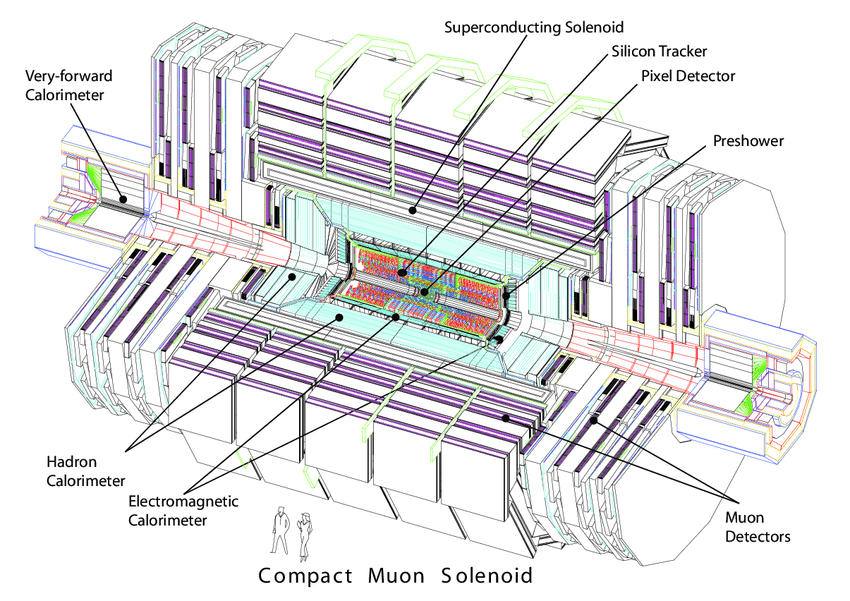
\includegraphics[width=.8\textwidth]{figures/lhc/detector_cms.png}
%     \caption{Overview of the \cms detector \copyright{\cern}}
%     \label{fig:detector_cms}
% \end{figure}

The \alice (A Large Ion Collider Experiment) \cite{other:alice} focuses on heavy ion collisions. It is designed to measure the physics of strongly interacting matter and the quark-gluon plasma at extreme energies and temperatures. It consists of a central barrel which covers polar angles from 45$^\circ$ to 135$^\circ$ and a forward muon spectrometer covering 2$^\circ$ to 9$^\circ$. While the \alice physics program includes the study of light atoms, the main study utilises heavy nuclei Lead-Lead collisions. Its first collisions was recorded in November 2010.

% \begin{figure}[t]
%     \centering
%     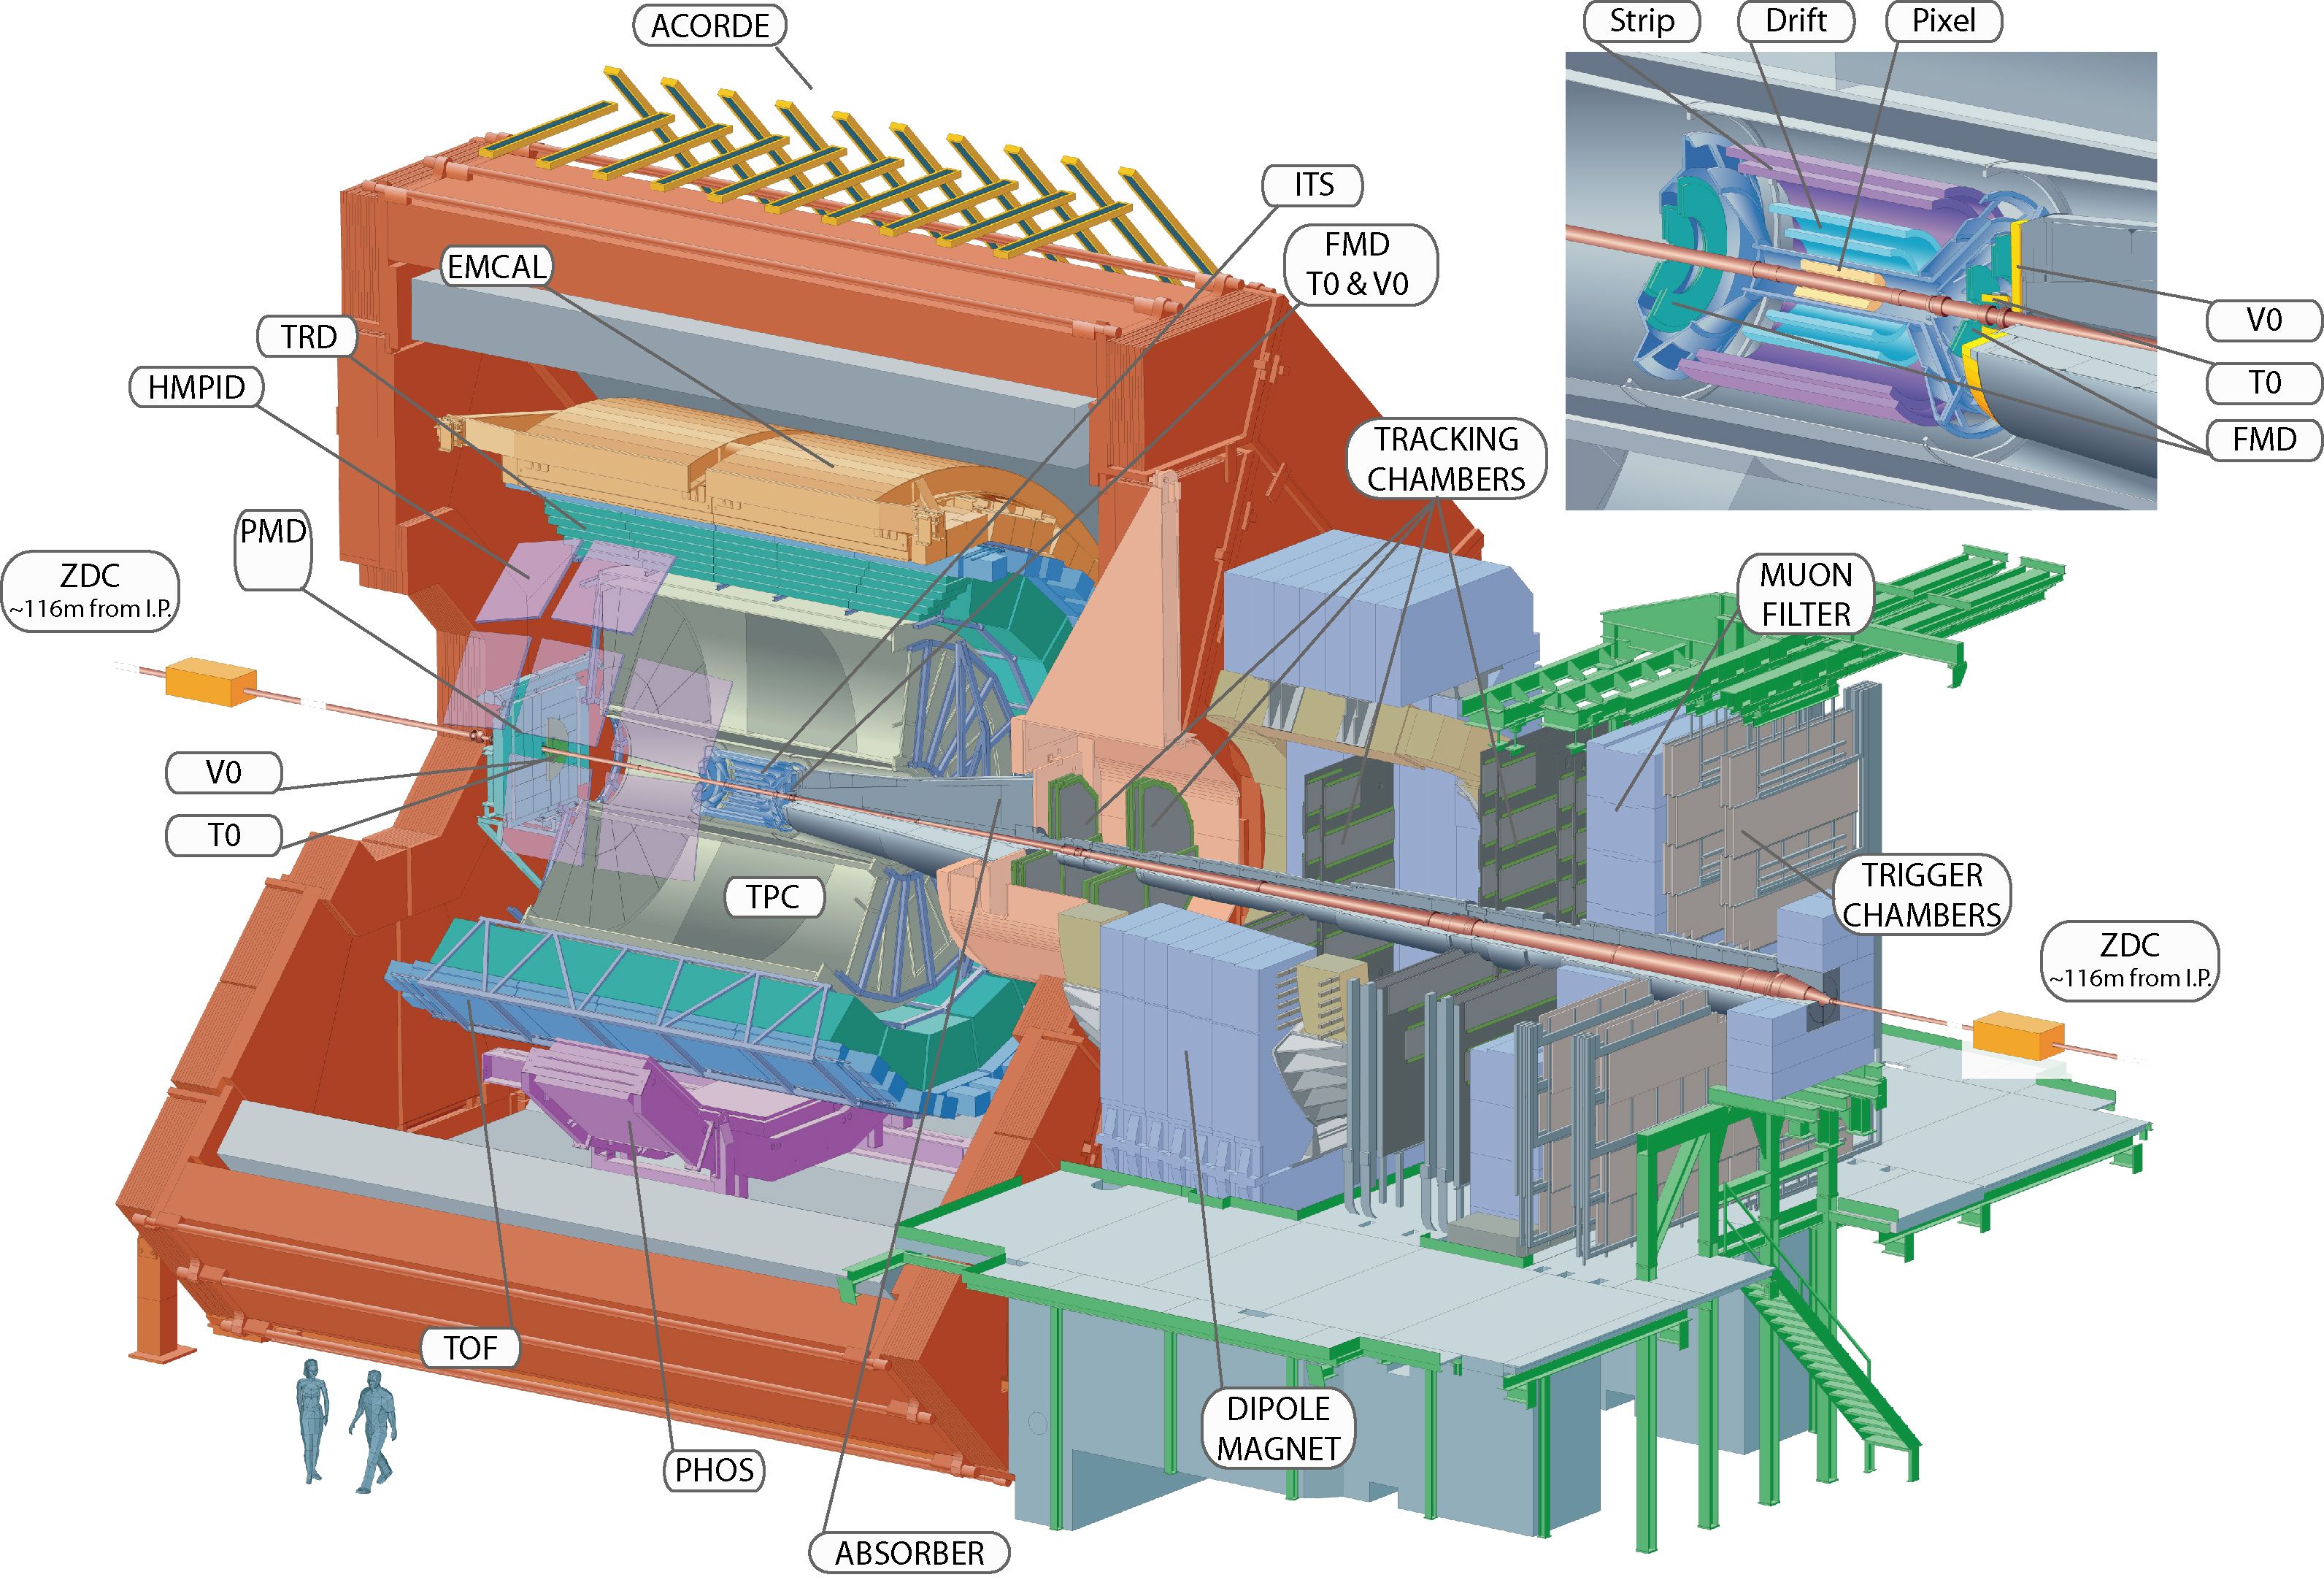
\includegraphics[width=.8\textwidth]{figures/lhc/detector_alice.jpg}
%     \caption{Overview of the \alice detector \copyright{\cern}}
%     \label{fig:detector_alice}
% \end{figure}

\lhcb (Large Hadron Collider beauty) \cite{other:lhcb} is dedicated to study particles that contain $b$ quarks, which sometimes are referred as beauty quarks. Unlike the other experiments, its detector is build as a single-arm spectrometer. It covers a forward angle of approximately 0.5$^\circ$ to 17$^\circ$. The reason lies in \lhcb's focus on detecting $b$ hadrons which are predominantly produced in forward and backward cones. The \lhcb experiment started the operation at the same time as \atlas and \cms.


% \begin{figure}[t]
%     \centering
%     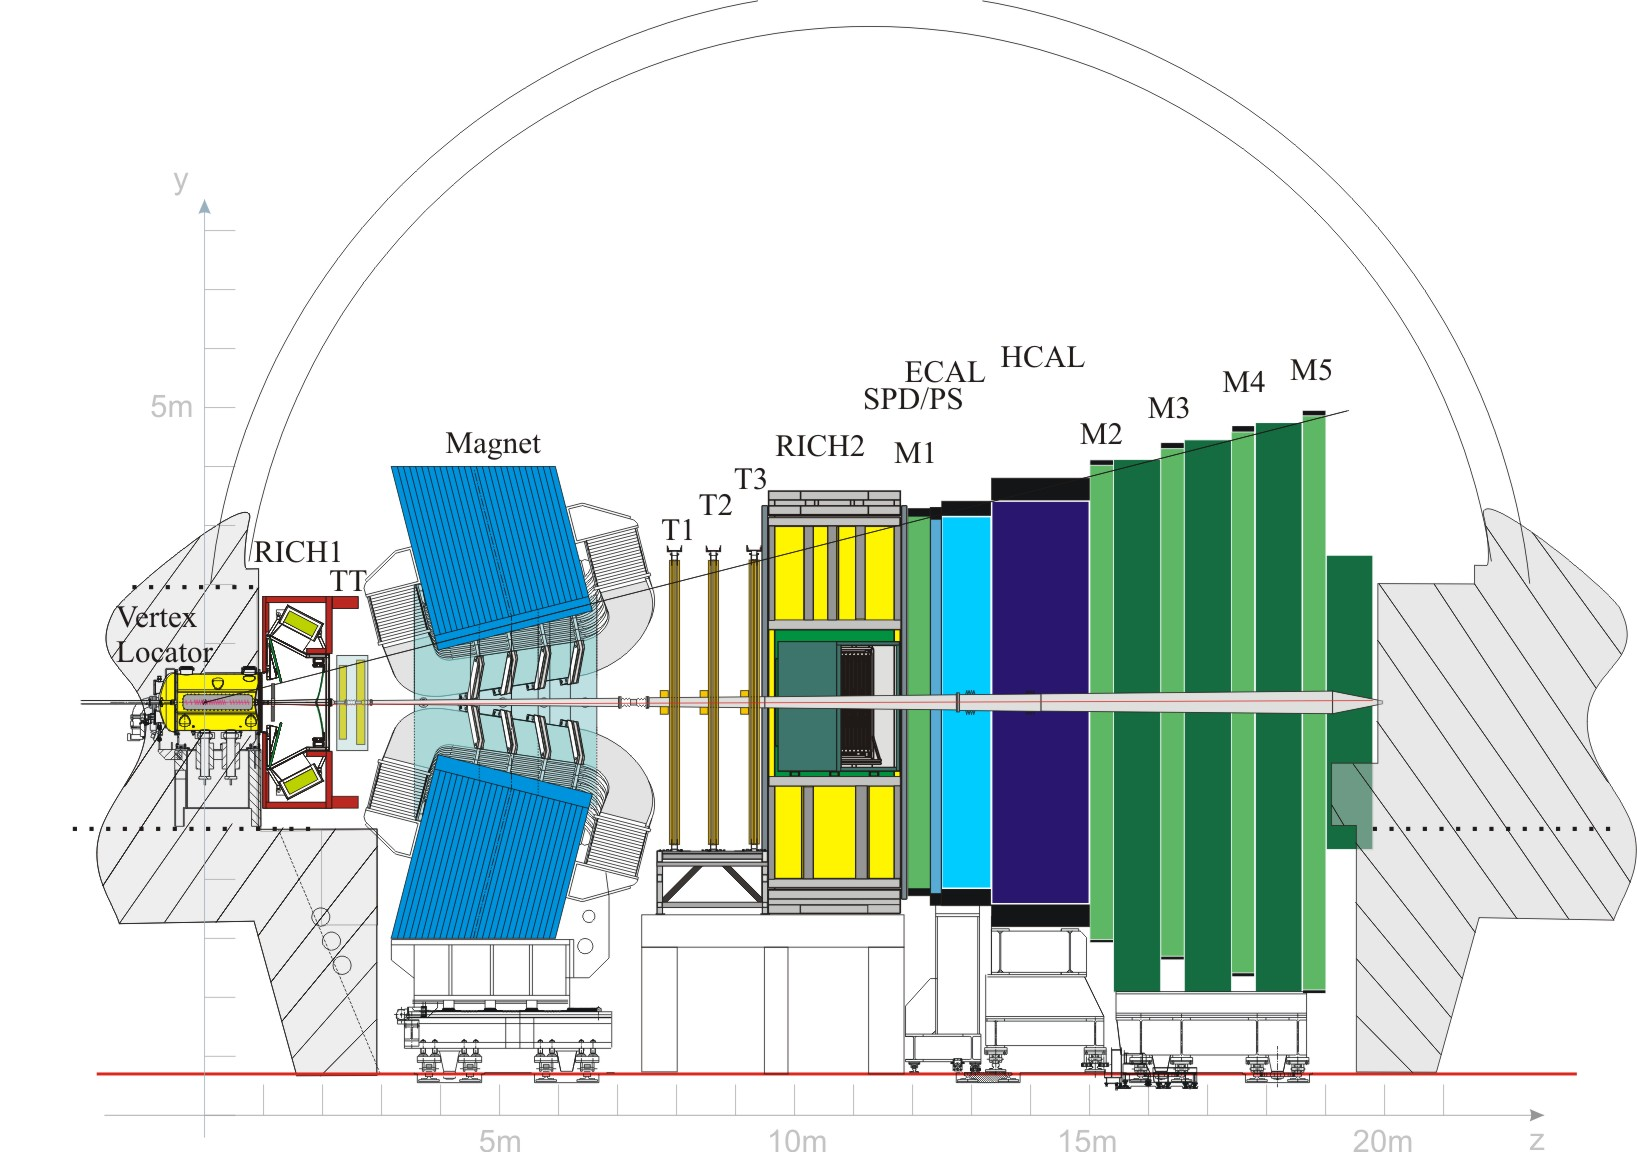
\includegraphics[width=.8\textwidth]{figures/lhc/detector_lhcb.jpg}
%     \caption{Overview of the \lhcb detector \copyright{\cern}}
%     \label{fig:detector_lhcb}
% \end{figure}

\chapter{Truth Matching}
\label{ch:truth_matching}
Training a neural network as explained in Chapter~\ref{ch:spanet} requires sufficient training samples. To generate such training samples, a truth matching algorithm is used. The algorithm takes the truth and reconstructed information of MC simulations as inputs, and outputs a jet-parton assignment that can be used for training. The following section gives a high-level explanation of the algorithm.

\section{Algorithm}
\label{sec:truth_matching:algorithm}
To produce the training data, the algorithm begins by scanning the input MC samples. Each sample includes truth information of the partons before interacting with the detector. The truth information also includes the true identification of particles as well as their decay products. Furthermore, the samples include the reconstructed information at detector level. Here, the particles and their properties are simulated as they would appear in data. Pairing the reconstructed and truth information of each event, allows generating training sets that uses the reconstructed information with true labels. 

The algorithm analyses each event by iterating through all truth-level final state partons. Around each of these partons, the algorithm searches possible jet matches. All jets within a spatial cone around a parton are considered as its candidate matches. Here, the cone is defined by $\Delta R\leq0.4$ as introduced in Section~\ref{sec:exp:atlas_coordinate_system}. For the targeted \ttHWW semileptonic final state, 8 quarks (3 per $t$ quark + 2 for the hadronic $W$-boson from the $H$-boson) have to be matched. 

If there is no jet within the cone of a parton, then that parton is not matched. If exactly one candidate is found inside the cone, the jet is saved as the final match for the jet-parton assignment. For cases with more than one candidate match, the jet closest to the particle in $\Delta R$ is chosen as the final match. 

Each matched jet is made unavailable for other partons. Hence, each jet-parton assignment is unique which is required for training the neural network. Afterwards, the algorithm proceeds to combine the matched particles. The four-vectors of the jets are added up to get the four-vector of the expected resonance particles.

Furthermore, several technical optimisations such as hashmaps and bit-shifting operations are implemented to increase the processing speed. To implement bit-shifting, each jet gets an integer number assigned. Each parton corresponds to one of the bits in the integers bit-representation. Bit values of 1 mean the jet is potentially matched to the corresponding parton, while 0 means that the parton is not included withing the jets $\Delta R$ cone. Each parton has a fixed position in the bit-representation. Hence, checking a potential parton-jet match is done efficiently by bit-operations.

\chapter{SPA-Net: Symmetry Preserving Attention Networks}
\label{ch:spanet}
This chapter introduces the transformer neural network \spanet \cite{spanet_01,spanet_02}, which is used for the hadronic jet-parton assignment during event reconstruction. Section~\ref{sec:spanet:chi_squared} first explains the classical approach for solving such assignment problems by using the $\chi^2$ minimisation technique. Then Section~\ref{sec:spanet:modern} presents the implemented neural network approach.

\section{Classical \texorpdfstring{$\chi^2$}{Chi Squared} Method}
\label{sec:spanet:chi_squared}
%For top analysis in particular, this was calculation was implemented in the KL-Fitter framework \cite{nn:kl_fitter}
Traditionally, to determine the jet-parton assignment of an event, a simple $\chi^2$ minimisation approach \cite{nn:chi_squared} is used. The method tests every possible combination of jets in the event, calculating the masses $m$ of the resonance particles ($t$,$W$,$H$) and then compares it to the SM prediction $M$. The methods tries to find the best matching mass for all resonance particles. Mathematically, for every assignment the following is calculated

\begin{align*}
    \chi^2 = \sum_{i,j} \frac{(m_{q_i}-M_j)^2}{\sigma_j^2}
\end{align*}

with $\sigma$ being the SM mass uncertainty. The lowest $\chi^2$ value corresponds to the best matching jets $i$ of each resonance particle $j$. Thus, it is expected to be the most accurate jet-parton assignment. 

This approach is not suited for the targeted event topology of this study. For the targeted \ttHWW channel, 8 jets are expected in the semileptonic final state. This leads to high numbers of permutations which slows down the calculation significantly. Even when introducing $b$-tagging and requiring the method to only swap $b$-tagged jets with other $b$-tagged jets, the algorithm would have $6!=720$ possible light jet permutations per event. Hence, this method is not implemented. Instead, a neural network is trained.

\section{Modern DNN Method}
\label{sec:spanet:modern}
In this study, the transformer-based deep neural network architecture \spanet (Symmetry Preserving Attention Networks) \cite{spanet_01,spanet_02} is used for predicting the jet-parton assignment. \spanet was originally developed for fully hadronic \ttbar analysis \cite{spanet_03}. However, the implemented network is extended to general event topologies \cite{spanet_01} and thus, can be used for the targeted \ttHWW topology.

Its task is to predict a jet-parton assignment for all jets in the targeted semileptonic final state. This hadronic assignment can then be combined with the leptonic estimation using \NW resulting in a full event reconstruction.

One of \spanets features is the utilisation of symmetries in the event topology. These symmetries are implemented in the loss function during training. The loss does not change under predefined symmetrical permutations. Symmetries are classified into two groups: jet and particle symmetries. 

The jet symmetry describes that labelling certain particles is symmetric and thus, changing their labels does not change their physical behaviour. In the \ttHWW topology, this symmetry is present in the hadronic $W$-boson decays which produce two quarks $q\bar{q}'$. %Their labels are set arbitrary and can be swapped without any change in the physical reconstruction. %Under the assumption that the $W$-boson couples evenly to both quarks, their labelling can be changed without any physical consequence. While this assumption ignores the parity violating properties of the $W$-boson \cite{theory:electroweak_01}, it is expected to serve as a practical approximation.

The particle symmetry depicts the symmetry with respect to the particle origin. Particles that originate from a quark or its respective anti-quark are symmetric, when disregarding their charge. For the targeted \ttHWW topology, the symmetry is applicable in the decays of either the $t$ or $\bar{t}$ quark. While there might be subtle differences in the hadronic charge distributions of the $t$ and $\bar{t}$ quarks, we do not expect to be able to resolve them. Hence, the jet assignment treats both particles equally.

By considering these symmetries, the number of possible permutations is reduced and the processing speed increases. The run-time is reduced to $\mathcal{O}(N_\text{jets}^3)$ compared to the baseline $\chi^2$ method with a expected run-time of $\mathcal{O}(N_\text{jets}^C)$ \cite{spanet_01}. Here, $N_\text{jets}$ are the number of jets within a given event and $C=8$ is the number of final state partons or $C'=6$ when separating $b$-tagged jets. 

\spanets network architecture is visualised in Figure~\ref{fig:spanet}. It can be subdivided into four components \cite{spanet_01}: input embeddings, central transformer, particle transformers and self-attention output layer.

\begin{figure}[t]
    \centering
    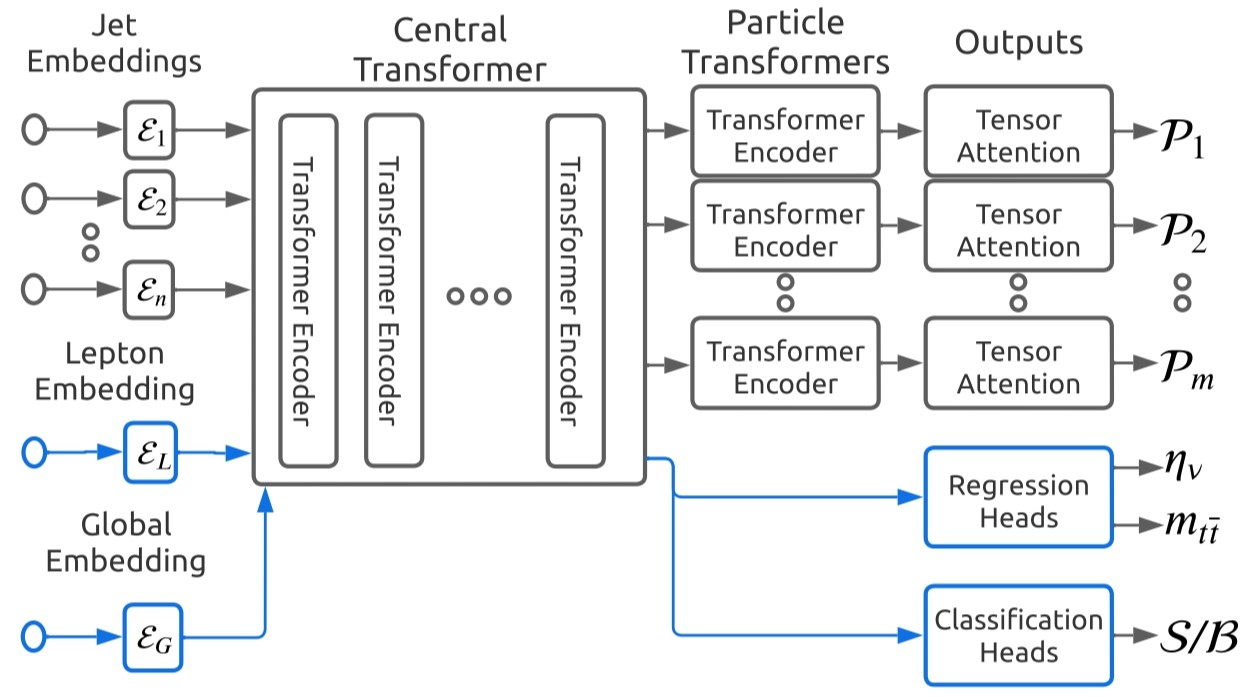
\includegraphics[width=.8\textwidth]{figures/methods/spanet_architecture_2.jpg}
    \caption{Overview of \spanets architecture including its four regions and the additional embeddings for additional lepton and global information such as the missing transverse energy \cite{spanet_02}.}
    \label{fig:spanet}
\end{figure}

During training, each prediction is split into three steps. First, the amount of valid jet assignment permutations is reduced by splitting up events into sub-structures which are predefined by the event topology. Then each jet-parton assignment sub-problem is solved by applying a `Symmetric Tensor Attention' \cite{spanet_01} layer, producing a single tensor. Each tensor is a multi-dimensional array. These tensors contain an entry for each sub-assignment including the probability that any particular combination is the correct sub-assignment. These tensors are combined into a final jet-parton prediction by calculating the combined symmetric loss \cite{spanet_01}. The approach of splitting up the individual particles allows partial event reconstruction which is vital for this study. 

Particle symmetries are implemented in the symmetric cross entropy loss during training. Changes which obey these symmetries do not change the loss value. This behaviour is achieved by allowing the network to train any equivalent assignment as long as the overall loss is minimised. Jet symmetries are included in permutation groups which are used by the Symmetric Tensor Attention layer \cite{spanet_01}. The attention refers to \spanets ability to dynamically weight different parts of the input to improve the overall performance by focusing on relevant features.

During inference, the combined symmetric loss is not calculated. Instead, \spanet iteratively assigns jets to the to expected particles by selecting the most likely assignment from each output tensor $\mathcal{P}_p$. The used permutations are bijective to ensure a unique jet-parton assignment \cite{spanet_01}. Hence, in cases where one jet is assigned more than once, the highest probability score is selected and the others are evaluated again.

In comparison to other techniques, \spanet offers several advantages. Firstly, \spanet is agnostic to the number of input objects. Hence, training and prediction can be done using samples containing any jet multiplicity. Secondly, all predicted jet matches are unique. Furthermore, each prediction is also rated using an assignment probability that represents \spanets confidence for that particular prediction. And lastly, the expected symmetries due to the event topology are predefined which leads to significantly higher processing speed by simplifying the training and prediction task.

For training \spanet to the targeted topology, a suitable training sample is created using \ttbar and \ttH events. The needed truth-matching algorithm for creating such training samples is explained in Chapter~\ref{ch:truth_matching}.


\chapter{Neutrino Weighting}
\label{ch:neutrino_weighting}
\NW is a technique to reconstruct events including neutrinos in their final state. It was first implemented by the \dzero collaboration in dileptonic \ttbar events \cite{neutrino_weighting:original}. The kinematic reconstruction with neutrinos in the final state are underconstrained, due to the unmeasured neutrino particle. Hence, the reconstruction relies on certain assumptions. With these constraints, \NW yields an estimation of the unknown parameters by calculating the most likely combination of them. 

While the original \NW was developed for events with two neutrinos in the final state, this study adapts and modifies the original approach to reconstruct the leptonically decaying $W^*$-boson in the \HWW subprocess \cite{neutrino_weighting:adaptation}. For the targeted event topology, the free parameters are the mass, $m_{W^*}$, of the off-shell $W^*$-boson and the pseudo-rapidity, $\eta_\nu$, of the neutrino $\nu$. 

The algorithm outputs an estimation for these free parameters and a weight, $w$, which is in the range of $[0,1]$. Higher values describe a better agreement between the estimated values and the observed event kinematics. This weight can be used in the event selection to identify the targeted semileptonic \ttHWW topology.

\section{Parameter Estimation}
To apply the \NW algorithm, some assumptions need to be made to constrain the otherwise underconstrained \HWW sub-system. First, the $H$-boson is assumed to be on-shell. The used MC samples sets $m_H^\text{MC}$ to $125.0$\,GeV. When using real data, the measured mass, $m_H=(125.09\pm0.24)\,\text{GeV}$ from a combined \runi measurement is used \cite{higgs_mass_combined}. Additionally, the mass of the on-shell $W$-boson is fixed at $M_W=80.379\,\text{GeV}$ \cite{pdg}. Lastly, the on-shell $W$-boson is further assumed to decay hadronically. Then, the \HWW sub-system can be reconstructed by estimating the off-shell leptonic $W^*$-boson and combining it with the hadronic $W$-boson to form a Higgs boson.

To find the best estimation for the $W^*$-boson, several combinations of the off-shell mass, $m_{W^*}$, and the pseudo-rapidity of the neutrino $\eta_\nu$ are sampled using a grid-based search. The grid samples 100 $\eta_\nu$ points within $[-3,3]$ and 100 $m_{W^*}$ points within [$0,50$]\,GeV. All points are distributed equidistantly. The mass of the $W^*$-boson is limited to approximately 50\,GeV due to the on-shell constraints. While the pseudorapidity $\eta$ is not physically limited, the range $[-3,3]$ is selected to ensure optimal detector performance. The different pseudorapidity regions are explained in Ch.~\ref{ch:experimental_setup}.

Due to the assumptions, the \HWW sub-system is fully constrained \cite{neutrino_weighting:adaptation} and the neutrino transverse momentum $p_T^\nu$ can be calculated. This reconstructed neutrino momentum, $p_T^\nu$, can be compared to the observed missing transverse momentum, $p_T^\text{miss}$. For that, the transverse momenta are split into their two components $p_x$ and $p_y$ with $p_T^2=p_x^2+p_y^2$. The weight of one solution is calculated as

\begin{align}
    w = \exp{\frac{(p_x^\nu-p_x^\text{miss})^2}{\sigma_x^2}} \cdot \exp{\frac{(p_y^\nu-p_y^\text{miss})^2}{\sigma_y^2}}.
\end{align}

The variable $\sigma_{x/y}$ is the experimental resolution of the missing momentum $p_{x,y}^\text{miss}$ and only serves to scale the weight. Thus, it has no physical impact on the result if taken equal in $x$ and $y$ \cite{neutrino_weighting:adaptation}. The implementation sets  $\sigma_{x/y}=10\,$GeV. The value is chosen since it is the worst resolution at the \atlas detector for events with transverse energy up to approximately 100\,GeV \cite{atlas:met_resolution}. This is expected to be appropriate for the targeted event topology.

For each event the sampled $m_{W^*}$ and $\eta_\nu$ can be visualised together with the weight of each grid point to form a distribution as seen in Figure~\ref{FIG:neutrino_weighting:cherry_picked}. The maximum of this distribution corresponds to the most likely combination of the unknown parameters. White regions are kinematically forbidden and thus, no solutions can be found for these regions. 

\begin{figure}
    \centering  
    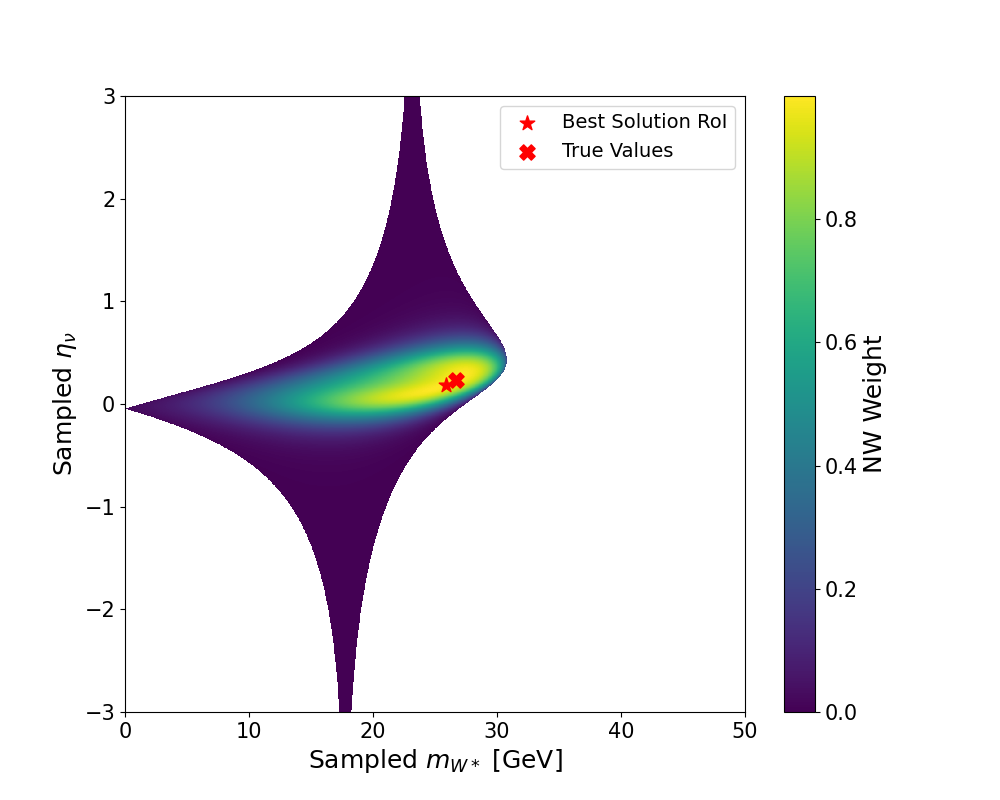
\includegraphics[width=0.7\textwidth]{figures/Neutrino Weighting/cherry_14.png}
    \caption{Example of a sampled weight distribution for a cherry-picked event. The highest weighted solution in the region of interest (star) and the true values (cross) are marked.}
    \label{FIG:neutrino_weighting:cherry_picked}
\end{figure}

\section{Optimisation}
\label{sec:neutrino_weighting:optimisation}
Since the targeted \ttHWW process is rare, it is crucial to maximise the number of reconstructable events. To increase these statistics as well as the accuracy of the estimated values for $m_{W^*}$ and $\eta_\nu$, two minor optimisations are implemented. These are explained briefly in the following sections. The improvement due to these optimisations is given in Sec.~\ref{sec:results:neutrino_weighting}.

\subsection*{Higgs Mass Smearing}
Some events do not yield any solution during the initial grid-based search. Hence, there is no estimation for $m_{W^*}$ or $\eta_\nu$. To decrease the amount of events with no solution, the assumed Higgs boson mass $m_H$. can be altered slightly. This approach is valid since reconstruction effects can change the measured energies of jets, leptons or the missing transverse energy. Then, the precise $H$-boson mass might not yield a solution. Then it is viable to also test masses close to the expected $m_H$ to counteract these reconstruction effects.

Hence, if an event has no solution, the assumed $H$-boson mass is varied in a range of $\pm1$\,GeV using 0.1\,GeV steps around $m_H$. The grid-based search is repeated for each alternative assumption $m_H'$. If any solution is found using the alternative Higgs mass $m_H'$, it is used to estimate $\eta_\nu$ and $m_{W^*}$.

This additional step increases the processing time for the \NW algorithm by $\sim$10-50\%. The specific time increase is dependent on the sample composition. Due to this additional step, around 1\% of events that would be rejected become reconstructable.

\subsection*{Regions of Interest}
As an additional improvement, the \NW algorithm defines regions of interest. These regions are used to refine the estimated solution. 

If the algorithm finds at least one solution during the grid-based search, an additional finer grid-based search is started around the highest weighted solution. This second grid is the local region of interest. Within the region of interest, the steps for $m_{W^*}$ and $\nu_\eta$ are more granular to find an even higher weighted, local solution. The final solution is the highest weighted estimation within the region of interest. 

If an event has two solution initially only the highest weighted solution is searched again using the region of interest. Hence, if the second highest weighted solution was the actual solution but was not estimated at precise enough values, the true solution is not found. 

The region of interest increase the processing time by $\sim$15\% independent of the sample composition. However, the average estimation accuracy when using this optimisation is increased by <0.1\%.



\chapter{Event Selection}
\label{ch:event_selection}
This chapter covers the event selection strategy used to separate the targeted semileptonic \ttHWW events from other background processes. Section~\ref{sec:event_selection:objects_of_target} introduces the event topology in greater detail and explains the assumptions used. Section~\ref{sec:event_selection:separation_power} defines the separation power and showcases some of the investigated variables. The behaviour of several event topologies is compared with respect to these variables. Lastly, sensitive variables are used in Section~\ref{sec:event_selection:region_definition} for the final region definition.  

\section{Objects of the Target Event Topology}
\label{sec:event_selection:objects_of_target}
The targeted semileptonic \ttHWW event topology is introduced in Sec.~\ref{sec:theory:tthww}. Its final state consists of eight jets and a single lepton-neutrino pair. Six of these jets originate from the \ttbar decays, while the remaining two jets stem from the $H$-boson decay sub-system. Among the eight jets, exactly two are tagged as $b$-jets which originate from the $t$ quark decay ($t \rightarrow Wb$). For the purposes of event reconstruction, three restrictions are made to improve the background rejection. 

Firstly, the \ttbar system is expected to decay fully hadronically. This implies that the observed lepton does not originate from the $t$ quark decay but instead is produced in the $H$-boson decay chain. Only then can the implemented \NW technique be applied properly.

Secondly, $H$-boson is produced on-shell due to the resonance production. Hence it is expected to have a mass of $m_H=(125.09\pm0.24)$\,GeV \cite{higgs_mass_combined}. The simulated MC samples were tested and the on-shell $H$-boson production dominates. Given the energy constraints, the $H$-boson cannot decay into two on-shell $W$-bosons. Therefore, one of the $W$-bosons must be off-shell. 

Lastly, the off-shell $W^*$-boson is expected to decay leptonically. This is crucial because, without the on-shell constraint on the hadronic $W$-boson, it would be almost impossible to assign the jets to the $W$-boson, as any combination of jets could potentially reconstruct an off-shell $W^*$-boson with an indeterminate mass.

This also means that the two jets assigned to the on-shell $W$-boson are expected to have an invariant mass close to the SM $W$-boson mass value of $M_W=80.37\pm0.02$\,GeV \cite{pdg}.

As explained in Sec.~\ref{sec:theory:tthww}, the primary background arises from \ttbar events, which have a significantly larger production cross-section compared to the signal \ttHWW events. \ttHbb and \ttHtautau events also contribute significantly, due to their comparatively high $H$ decay ratio of ($58\pm12$)\,\% and ($6.3\pm1.7$)\,\%, respectively \cite{yellow_report_4_higgs}. Additional backgrounds can arise from \ttHcc events and hadronic or dileptonic \ttHWW decays. These background processes are considered during the variable investigation and in the final region definition.

\section{Separation Power}
\label{sec:event_selection:separation_power}
To compare the performance of certain variables to separate signal and background, the corresponding distributions are displayed together. Here, the signal is defined to only include semileptonic \ttHWW events while the background includes everything else. Naturally, the background contains the majority of all events. For a fair comparison, both signal and background are normalised to unity and binned using the same edges. The choice of variables is physically motivated by identifying measurable differences in the signal and background processes.

Furthermore, the separation power $\mathcal{S}$ can be calculated using
\begin{align}
    \mathcal{S} &= \frac{1}{2} \sum_i^\text{bins} \frac{\left(s_i-b_i\right)^2}{s_i+b_i}\,.
\end{align}
For each bin $i$, the variables $s_i$ and $b_i$ equal the normalised signal and background fractions, respectively. Since the separation power $\mathcal{S}$ is dependent on the binning, the absolute value has no physical meaning. However, when choosing the same binning, the separation power of several variables can be compared to identify the best performing ones. 

\begin{table}
    \centering
    \caption{Summary of the investigated variables for the event selection sorted by their calculated separation powers $\mathcal{S}$.}
    \begin{tabular}{l|c}
        Investigated Variable & $\mathcal{S}$\\
        \hline
        Total Jet Multiplicity & 21.9\,\% \\
        \spanet $t$ Assignment Probability & 21.2\,\% \\
        \spanet $W_\text{had}$ Assignment Probability & 9.0\,\% \\
        \NW Reconstructable & 1.7\,\% \\
        Missing Transverse Energy $E_T^\text{miss}$ & 3.0\,\% \\
        Lepton Energy $E_\text{lep}$ & 1.2\,\% \\
        \NW Output Weight & 0.4\,\% \\
        $b$-Jet Multiplicity & 0.2\,\% \\
    \end{tabular}
    \label{tab:event_selection:separation_power}
\end{table}


\subsection*{Jet Multiplicities}
Figure~\ref{FIG:separation_power_plots:jet_multiplicities} shows two distributions of events per total jet and $b$-jet multiplicity, respectively. This analysis uses the 85\,\% working point for the $b$-tagging.

As expected, the distribution of \ttHbb events is peaking at higher $b$-jet multiplicity than any other distribution. While all distributions peak at 2 $b$-jets, the \ttHbb event distribution peaks at 3 $b$-jets due to the two additional $b$-quarks in the final state. The $b$-jet separation power $\mathcal{S}=0.2\,\%$ is relatively low. The reason for this is that most background processes expect the same number of $b$-jets. Only the \ttHbb background can be separated efficiently from the signal using this variable.

The total number of jets shows similar distributions for all events. \ttbar events slightly favours low jet multiplicities which can be explained by this final state containing only 6 jets. The targeted semileptonic \ttHWW final state contains 8 jets. Moreover, hadronic \ttHWW events contain 10 jets in their final state. Hence, the number of jets can be used to separate some of the backgrounds from the signal and each other. However, due to additional jets or jets lost during reconstruction, the distributions do not clearly peak at their expected jet multiplicities. The separation power $\mathcal{S}=21.9\,\%$ is the highest value of all investigated variables. This supports the importance of this variable for separating signal from background.

\begin{figure}
    \centering
    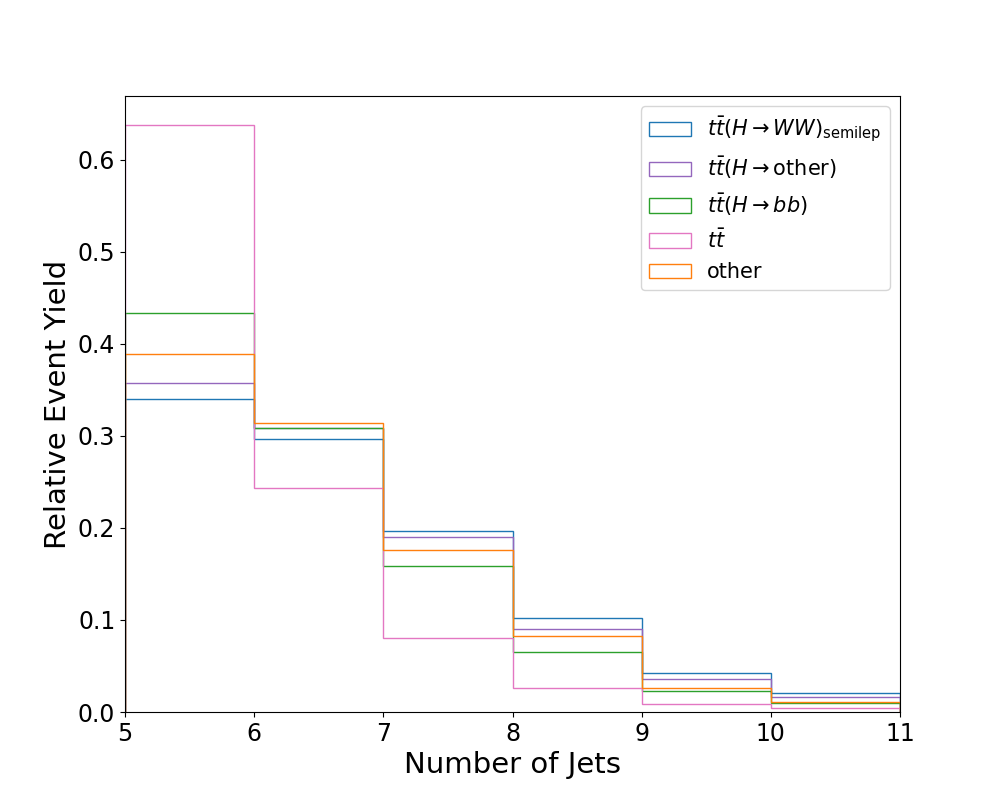
\includegraphics[width=.49\textwidth]{figures/separation_power/separation_splitnew_number_of_jets.png}\hfill
    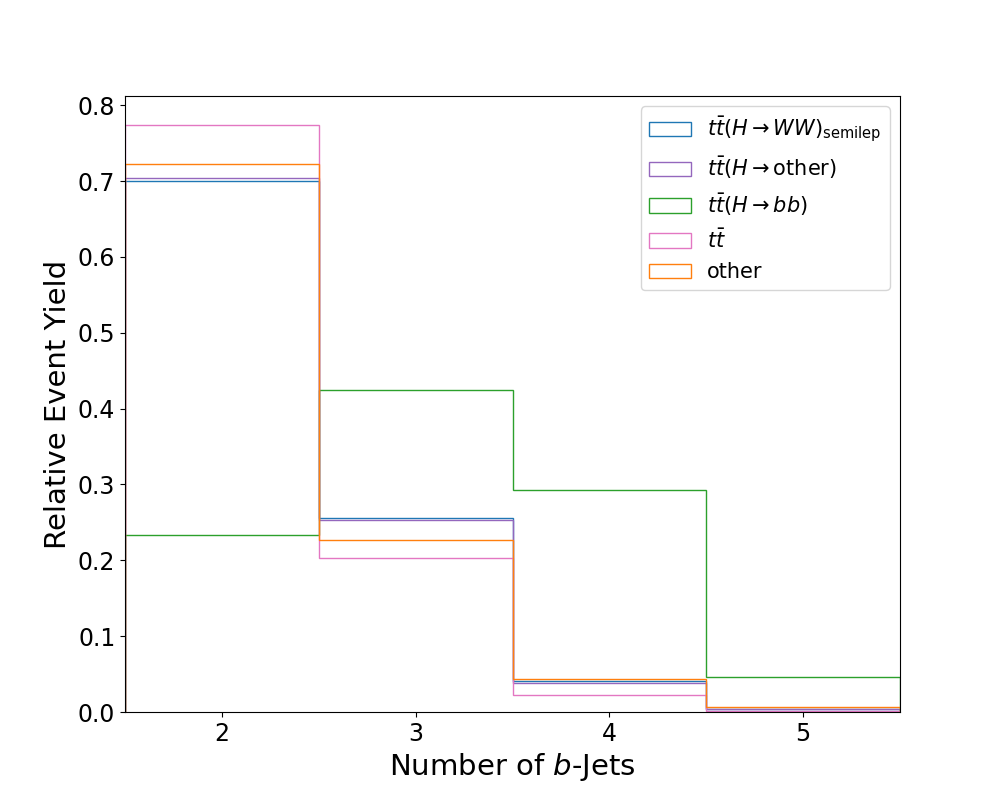
\includegraphics[width=.49\textwidth]{figures/separation_power/separation_splitnew_number_of_bjets.png}
    \caption{Distributions of different event topologies for (left) the total jet multiplicity and (right) the $b$-jet multiplicity per event.}
    \label{FIG:separation_power_plots:jet_multiplicities}
\end{figure}

\subsection*{Lepton Energies}
The distributions in Figure~\ref{FIG:separation_power_plots:lepton_energies} show the behaviour of different event topologies for the lepton energies $E_\text{lep}$ and missing transverse energies $E_T^\text{miss}$. 

The implemented single lepton triggers require at least one jet for selecting an event. This is combined with a lepton restriction which rejects more than one lepton. Therefore, every event contains exactly one lepton and thus, the choice of lepton is unambiguous.

For the missing transverse energy $E_T^\text{miss}$, the targeted semileptonic \ttHWW events peak approximately 10\,GeV lower than most other processes. In these events, the missing energy is expected to originate from the neutrino decay within the \HWW sub-system. Hence, $E_T^\text{miss}$ is limited by the energy of the leptonic $W^*$-boson decay. The separation power reaches $\mathcal{S}=3.0\,\%$ which corresponds to a similar sensitivity to signal and background.

The energies of the lepton $E_\text{lep}$ show a behaviour similar to $E_T^\text{miss}$. The targeted semileptonic \ttHWW events generally have lower lepton energies. However, here the dileptonic \ttHWW events behave very similar to the semileptonic decays. This similarity is expected since the production of the leptons is identical for both the semileptonic and dileptonic decay mode. Here, the separation power is $\mathcal{S}=1.2\,\%$ which is caused by the very similar behaviour of the dileptonic \ttHWW and \ttHtautau backgrounds. The dileptonic \ttHWW can separated by $E_T^\text{miss}$ since these events contain two neutrinos and thus, generally higher $E_T^\text{miss}$.

\begin{figure}
    \centering
    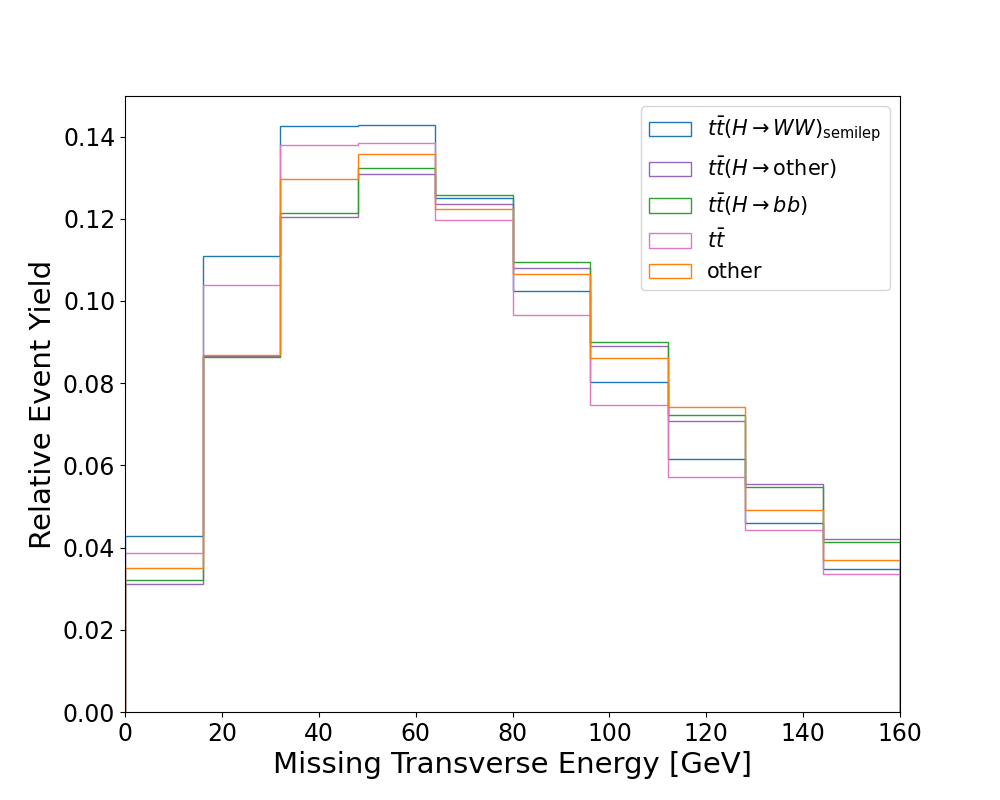
\includegraphics[width=.49\textwidth]{figures/separation_power/separation_splitnew_reco_met_value_gev.png}\hfill
    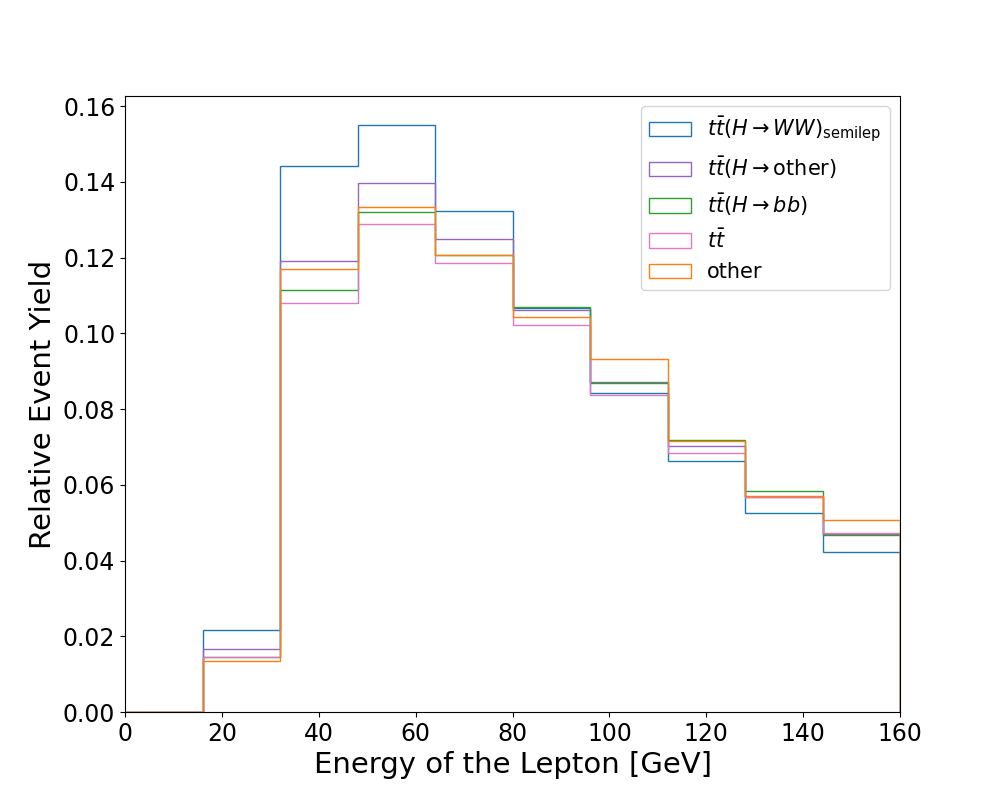
\includegraphics[width=.49\textwidth]{figures/separation_power/separation_splitnew_reco_lepton_e_gev.png}
    \caption{Distributions of different event topologies for (left) the missing energy per event and (right) the energy of the identified lepton.}
    \label{FIG:separation_power_plots:lepton_energies}
\end{figure}

\subsection*{SPA-Net Output Probabilities}
Figure~\ref{FIG:separation_power_plots:spanet_output_probabilities} includes two distributions of \spanets output probabilities. These probabilities are calculated during the jet assignment prediction. Events with high probabilities are more likely to be correctly matched. Both the $t$ and the $W_\text{had.}$ assignment probabilities show significantly different behaviours for the event topologies. 

The $t$ assignment proability generally is higher for the semileptonic and dileptonic \ttHWW events, which peak at 0.7 and 0.6, respectively, while \ttbar events score the lowest. The \ttHbb events also peak at 0.05 which is caused by the two additional $b$ quarks. These $b$ quarks from the $H$-boson decay can be misidentified as the $b$ quark from the $t$ quark decays. The average of both $t$ quark assignment probability is $\mathcal{S}=21.2\,\%$ which is the second highest separation power of all considered variables.  

Similarly, the $W_\text{had.}$ assignment probability also separates the different events topolgies. However, the distributions are not as clearly separated compared to the $t$ assignment probabilities. Here, \ttbar and \ttHbb peak at around 0.3 while the semileptonic \ttHWW peaks at 0.55. This variable reaches a separation power of $\mathcal{S}=9.0\,\%$. Compared to $\mathcal{S}$ of the $t$ assignment probability, this variable is less sensitive to signal. Due to their large separation power, these variables will be used in the region definition.

\begin{figure}
    \centering
    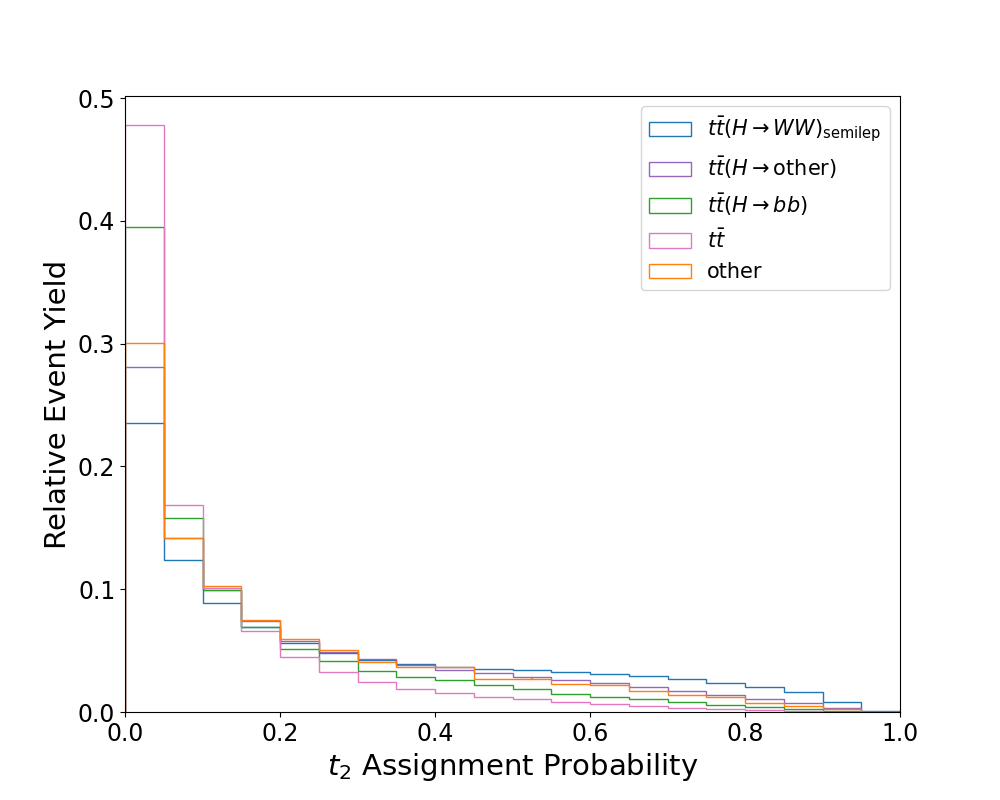
\includegraphics[width=.49\textwidth]{figures/separation_power/separation_splitnew_spanet_t2_assignment_probability.png}\hfill
    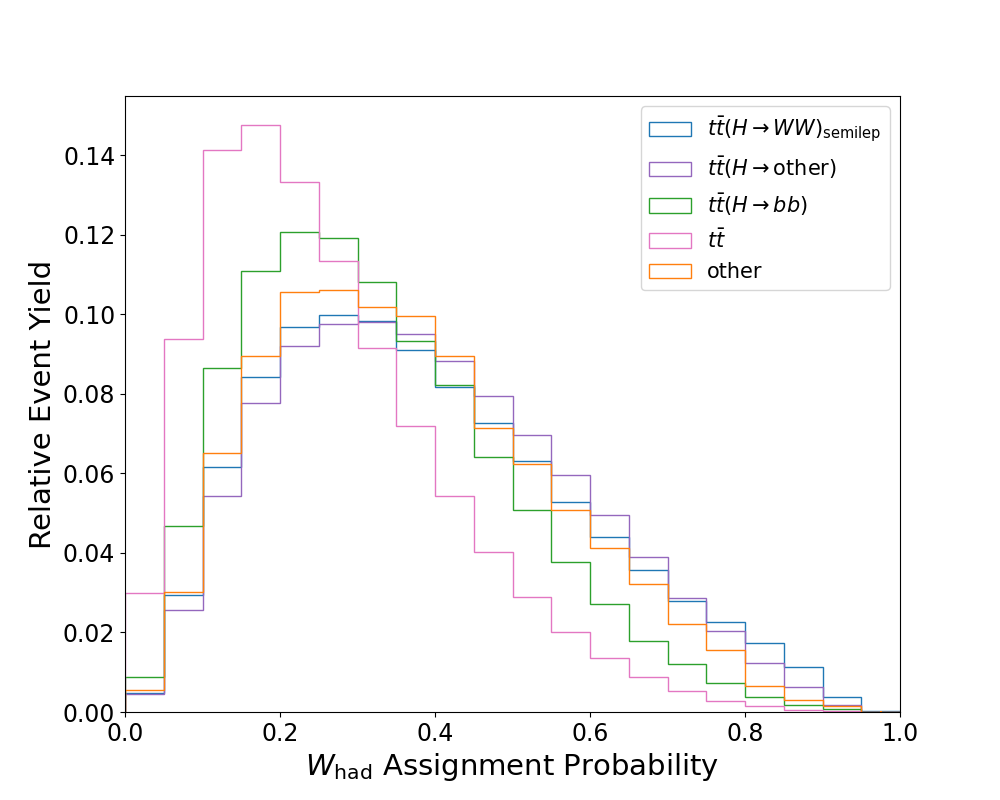
\includegraphics[width=.49\textwidth]{figures/separation_power/separation_splitnew_spanet_HW_assignment_probability.png}
    \caption{Distributions of different event topologies for \spanets assignment probabilities of (left) the top $t_2$ and (right) the hadronic $W$-boson from the Higgs decay.}
    \label{FIG:separation_power_plots:spanet_output_probabilities}
\end{figure}

\subsection*{Neutrino Weighting Output}
After estimating the unknown parameters of the event structure, the \NW algorithm outputs a weight. Visualising the distribution of the weights in Fig.~\ref{FIG:separation_power_plots:neutrino_weights} shows its separating power. Here the weight can be used to identify reconstructable and non-reconstructable events as well as quantify the reconstruction quality. Events with at least one solution are labeled as reconstructable and higher weights correspond to better estimations. 

Separating events with and without \NW solution yields a separation power $\mathcal{S}=1.7\,\%$. Looking at the weight distribution of all reconstructable yields $\mathcal{S}=0.4\,\%$. In comparison to the \spanet output probabilities, the separation power is lower and thus, does not separate the signal as efficiently. However, the \NW weight can still be used to separate signal events, when combining it with \spanets probabilities. 

\begin{figure}
    \centering
    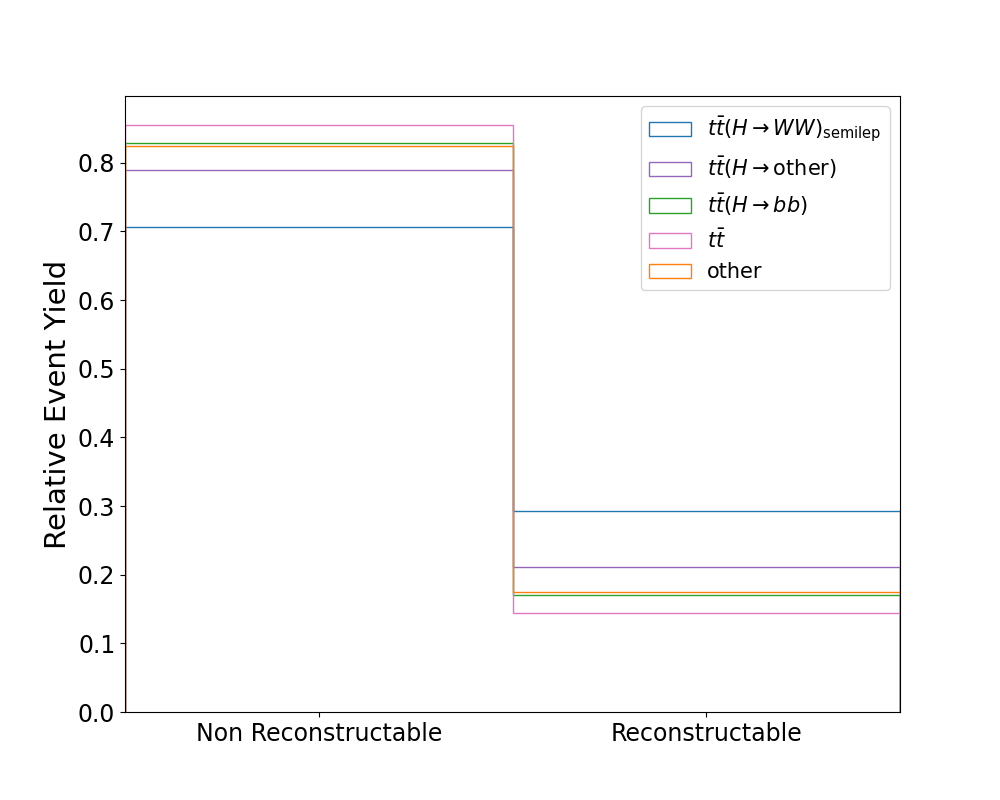
\includegraphics[width=.49\textwidth]{figures/separation_power/separation_splitnew_NW_weight.png}\hfill
    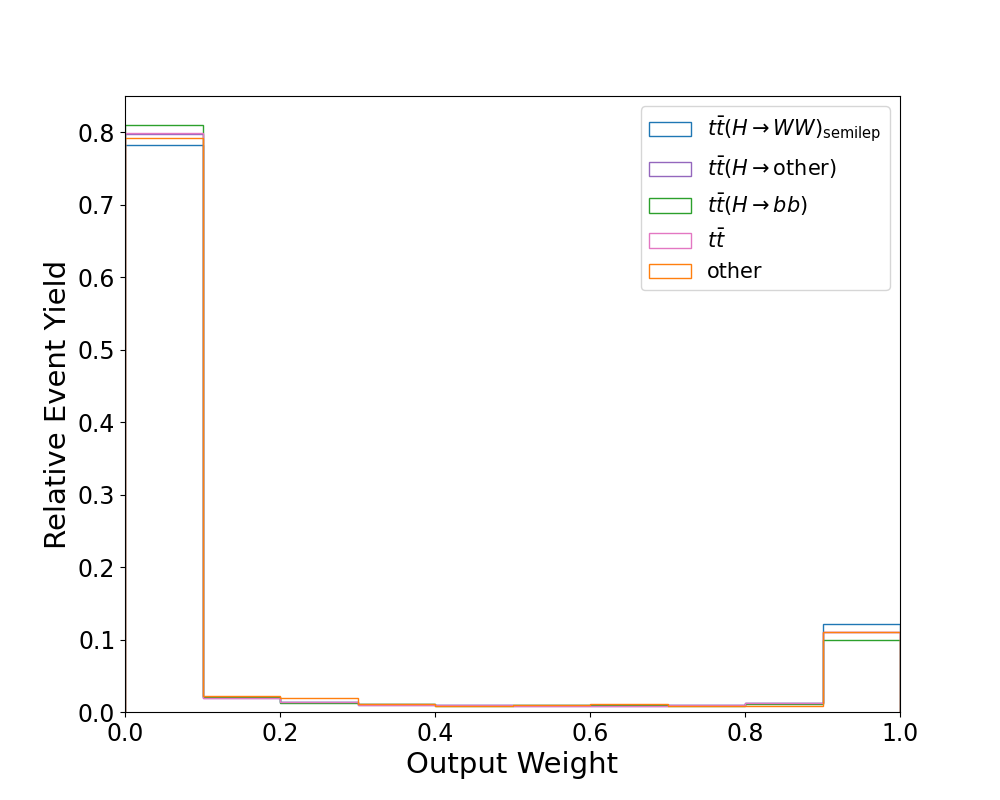
\includegraphics[width=.49\textwidth]{figures/separation_power/separation_splitnew_short_NW_weight.png}
    \caption{Distributions of different event topologies for \NW output weight while (left) including events without any solution and (right) excluding events without any solution. Events with no solution are visualised as negative weight.}
    \label{FIG:separation_power_plots:neutrino_weights}
\end{figure}


% \section{Event Preselection}
% During the event selection initial cuts to the whole dataset are applied. This reduces the overall yield while enhancing the signal purity when choosing the cuts carefully. Again, the choice of variables used for the preselection is physically motivated. Moreover, the qualitative cuts applied to each variable is based on their ability to capture signal and exclude background which is determiend by their separation power.
% Improving the signal-to-background ratio is crucial for rare processes such as the targeted semileptonic \ttHWW process. All cuts of the event selection as well as their impact on the relative event yield and signal purity are summarised in Table~\ref{TAB:EVENT_CLASSIFICATION:event_selection}. The final selection of cuts is conservatively focused on retaining as much of the signal as possible. The signal purity is based on predictons using MC samples and thereby is only an estimation of the true signal ratio in the dataset.
% \begin{table}
%     \centering
%     \caption{List of the selection used during event preselection. Only events that pass all cuts are used in the analysis. The relative yield is based on the dataset while the signal purity is estimated by using MC samples.}
%     \begin{tabular}{l|c|c}
%         Cut & rel. yield & signal purity\\
%         \hline
%         $n_\text{Jets}$>6 & XX.X\% & XX.X\\
%         $n_{b-\text{jets}}$>2 & XX.X\% & XX.X\\
%     \end{tabular}
%     \label{TAB:EVENT_CLASSIFICATION:event_selection}
% \end{table}


\section{Region Definition}
\label{sec:event_selection:region_definition}
To separate signal and background, the overall phase space is subdivided in signal regions $SR$ and control regions $CR$. If defined properly, the signal region is expected to include a relatively high purity of the targeted semileptonic \ttHWW events while excluding as much of the background contamination as possible. The control regions contain the remaining events with high background yields. Each control region targets one of multiple background processes. Only events where the \NW algorithm yields a prediction for the unknown neutrino and leptonic $W^*$-boson are reconstructable. Hence, only the events with a \NW solution are selected in the following. Given the rarity of the \ttHWW process, it is important that the union of all regions covers the entire remaining phase space to avoid discarding events. 

The $SR$ and $CR$ are constructed to be orthogonal. The choice of variables is driven by their respective separation power. The values at which the regions selects events are determined by using a grid search. An overview of all region definitions is given in Tab.~\ref{TAB:EVENT_CLASSIFICATION:regions} with the resulting region compositions given in Tab.~\ref{tab:event_selection:regions}. Furthermore, the ratios $S/B$ and $S/\sqrt{B}$ are calculated to show the signal purity and its statistical significance. Here, $S$ and $B$ correspond to the signal and background events, respectively.   

\begin{table}
    \centering
    \caption{Overview of the defined signal and control regions and their corresponding cuts. The conditions of the CR$_{t\bar{t}}$ marked with * are disjunctive, meaning only one them must be fulfilled. }
    \begin{tabular}{l|c|cc|c}
        & $SR$ & \multicolumn{2}{c|}{$CR_{t\bar{t}}$} & $CR_{H\rightarrow bb}$ \\
        \hline
        Total Jet Multiplicity                          & $\geq$7   & <8   & $\geq$7 & --- \\
        $b$-Jet Multiplicity                            & $\leq$3       & =2   & --- & $\geq$3 \\[2mm]
        \NW Reconstructable                             & yes       & any  & any & any \\
        \NW Output Weight                               & $\geq0.2$ & ---  & <0.2* & --- \\[2mm]
        \spanet $t$ Assignment Probability              & $\geq0.4$ & ---  & <0.4* & --- \\
        \spanet $W_\text{had}$ Assignment Probability   & $\geq0.4$ & ---  & <0.4* & --- \\
        \spanet $W_\text{had}$ Detection Probability    & $\geq0.7$ & ---  & <0.7* & --- \\
    \end{tabular}
    \label{TAB:EVENT_CLASSIFICATION:regions}
\end{table}

\begin{table}
    \centering
    \caption{Summary of all signal and control region compositions.}
    \begin{tabular}{l|c|c|c}
        & $SR$ & $CR_{t\bar{t}}$ & $CR_{H\rightarrow bb}$ \\
        \hline
        Event Count & 140 & 4764069 & 1346247\\
        Relative Yield & $0.0023\,\%$ & $77.97\,\%$ & $22.03\,\%$\\[2mm]
        $S/B$   & 0.008 & <0.001 & <0.001\\
        $S/\sqrt{B}$   & 0.095 & 0.22 & 0.23\\[2mm]
        Contribution \ttHWWlvqq  & 0.80\,\% & 0.01\,\% & 0.02\,\%\\
        Contribution \ttHbb & 0.12\,\% & 0.03\,\% & 0.27\,\%\\
        Contribution \ttHother & 0.24\,\% & 0.03\,\% & 0.06\,\%\\
        Contribution \ttbar & 98.84\,\% & 99.93\,\% & 99.65\,\%\\
    \end{tabular}
    \label{tab:event_selection:regions}
\end{table}

% \begin{figure}
%     \centering
%     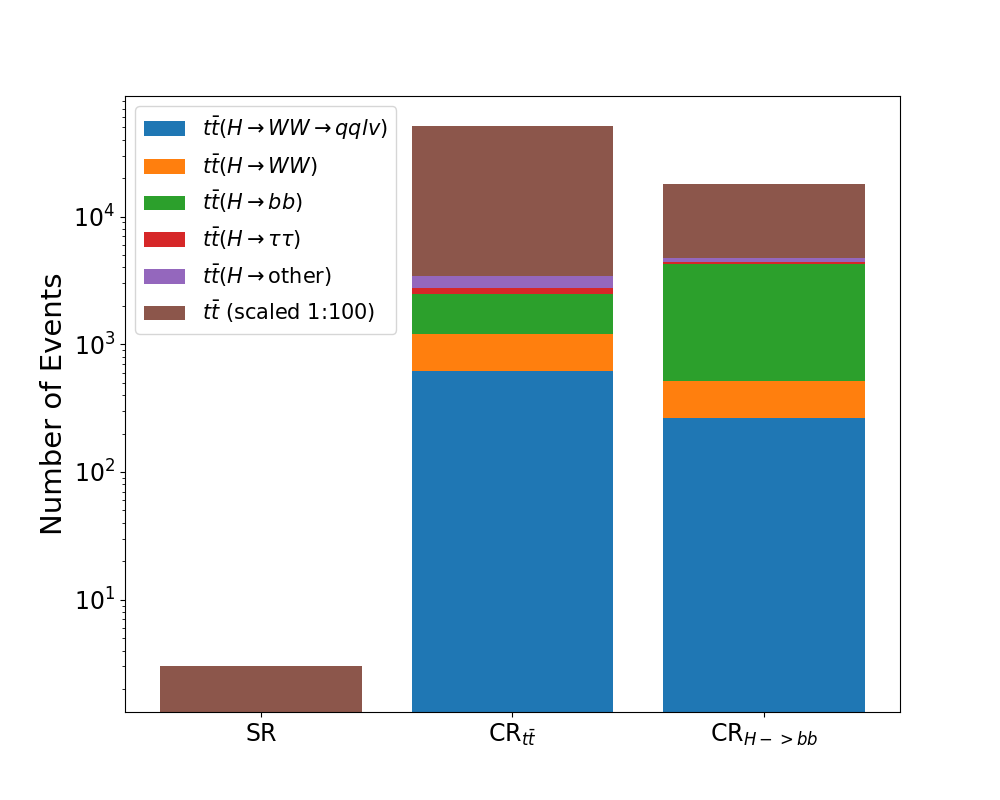
\includegraphics[width=0.6\textwidth]{figures/event_selection/regions.png}
%     \caption{Overview of the event composition of each signal and control region. The dominating \ttbar background is scaled 1:100 for visual clarity.}
%     \label{FIG:event_selection:regions}
% \end{figure}

\subsection*{Variable Combination}
To increase the performance of the outputs from \spanet and the \NW algorithm, the distributions are combinated in several 2-dimensional histrograms. In Fig.~\ref{FIG:separation_power_plots:abcd} the histrogram for the $t$ assignment probability and the \NW weight is shown for signal and background events.

\begin{figure}
    \centering
    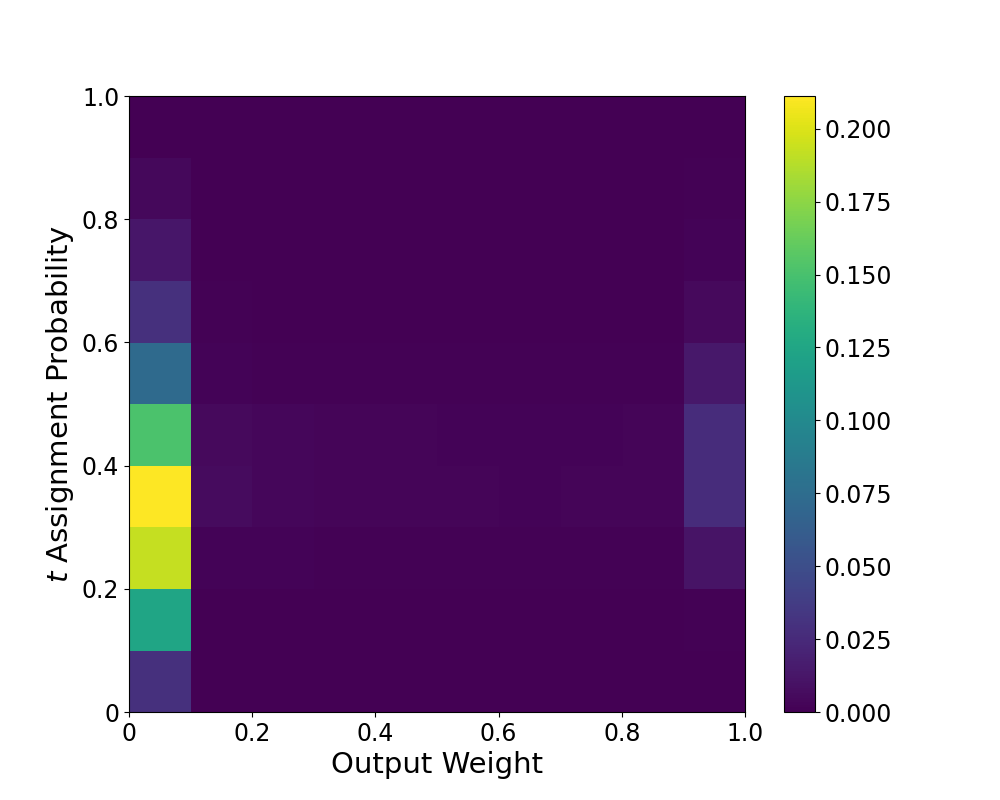
\includegraphics[width=.49\textwidth]{figures/abcd/abcd_background_$t$ Assignment Probability.png}\hfill
    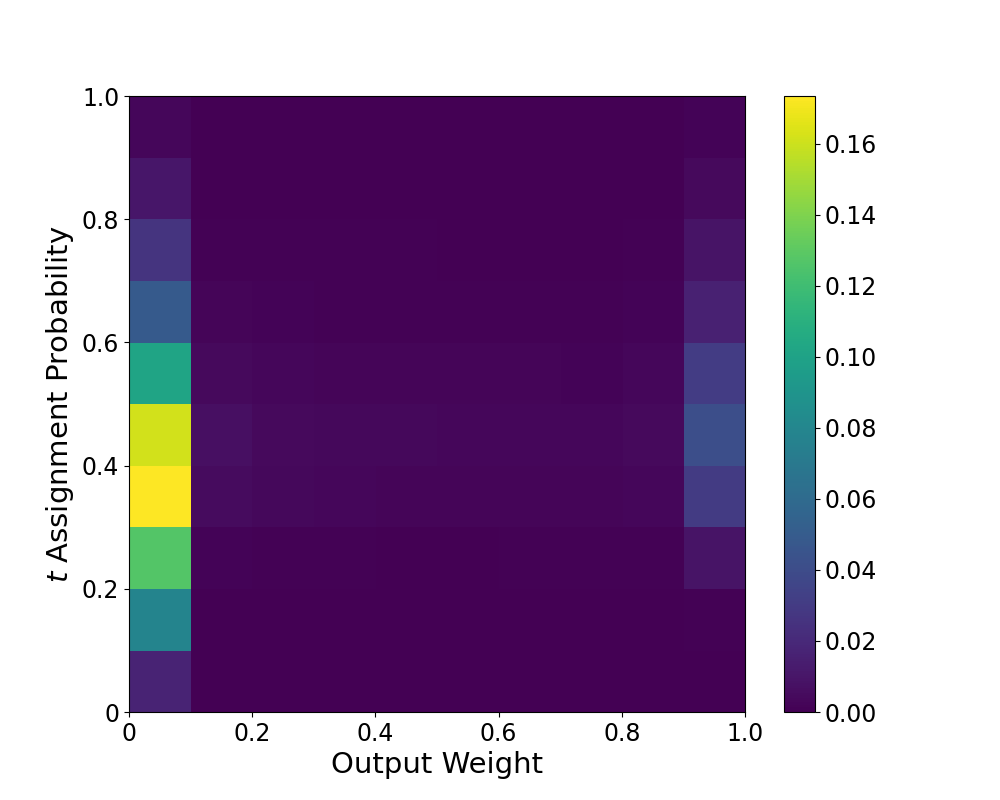
\includegraphics[width=.49\textwidth]{figures/abcd/abcd_signal_$t$ Assignment Probability.png}
    
    \includegraphics[width=.49\textwidth]{figures/abcd/abcd_background_$W_.text{had}$ Assignment Probability.png}\hfill
    \includegraphics[width=.49\textwidth]{figures/abcd/abcd_signal_$W_.text{had}$ Assignment Probability.png}
    \caption{Histogram combining \spanets assignment probability and \NW outputs for (left) background events and (right) signal events. here the partons are split into (upper) $t$ quark and (lower) $W_\text{had}$ from $H$-boson decay. The signal events have higher contributions in upper probability and weight regions.}
    \label{FIG:separation_power_plots:abcd}
\end{figure}


\subsection*{Signal Region}
One $SR$ is defined to separate as much signal events from background contamination as possible. As listed in Tab.~\ref{TAB:EVENT_CLASSIFICATION:regions}, the signal region mainly combines the outputs from \spanet and \NW. In addition to that, a conservative selection on the jet multiplicity is applied to retain enough signal events which expect at least seven jets in the final state of which three or less are $b$-tagged.

The selection results in a background rejection of 99.998\,\% while retaining a signal acceptance of 0.12\,\% for $SR$. After applying the proper event weights derived from SM prediction, the signal region contains 140 events with a signal purity $S/B$ of 0.80\,\%. However, due to the low event count in $SR$, the significance $S/\sqrt{B}$ is low compared to the $CR$s. Further increases in purity reduced the statistical significance of $SR$ drastically. The $SR$ is dominated by the \ttbar background with over 98,\% contribution due to its high cross-section.

\subsection*{Control Regions}
Two additional $CR$s, $CR_{t\bar{t}}$ and $CR_{H\rightarrow bb}$, are defined to separate \ttbar and \ttHbb events, respectively. 

For the $CR_{H\rightarrow bb}$ control region, the $b$-jet multiplicity is of particular interest. Since it is the only background process at leading order \ttbar and \ttH with a higher expected number of $b$-quarks in the final state, it can be separated by cutting events with at least three $b$-jets detected. The singular selection yields a \ttHbb acceptance of 75.0\,\% while including 22.03\,\% of all events. Moreover, 20.8\,\% of all signal events are selected by $CR_{H\rightarrow bb}$ which corresponds to a signal contribution of 0.02\,\%. While the significance $S/\sqrt{B}$ is relatively high, the signal purity $S/B$ is low.

The final control region $CR_{t\bar{t}}$ contains the majority of events with almost five million events. This corresponds to 77.97\,\% of all events. This region accepts 70.0\,\% of signal events which corresponds to a signal contribution of 0.01\,\% due to the high number of other events. As expected, the signal purity is drastically lower compared to $SR$ while containing higher statistics. 


\chapter{Results}
\label{ch:results}
In this chapter, the results of this study are summarised. First, the validation and performance of the truth matching script are stated in Section~\ref{results:truth_matching}. Sections~\ref{sec:results:spanet} and \ref{sec:results:neutrino_weighting} list the results from implementing \spanet and \NW, respectively. The final Section~\ref{results:data} includes the final results from combining all analysis steps and applying them on real data.

\section{Truth Matching}
\label{results:truth_matching}
This section briefly summarises the validated performance for the truth matching algorithm. The focus for this algorithm is set on producing unbiased jet-parton matches. While a higher truth matching performance is beneficial for creating sufficient training sets, it is not as crucial to optimise for the overall analysis since \spanet is also able to learn using partial events. Hence, only some optimisations were implemented and tested. 

\subsection*{Final Jet Selection}
During the matching process, a parton might have more than one potential jet to match. In this case, a metric needs to be defined to decide which jet is chosen as the matched reconstructed object. For that reason, final assignment in the case of multiple jet candidates is tested by using three different assignment schemes. 

The first matching scheme compares only the spatial separation between the potential jets and the targeted particle. The closest jet when calculating $\Delta R$ in respect to the parton is selected as the final match. The second approach utilises only |$\Delta p_T$| of the potential jets and the targeted particle. Here, the closest pair in momentum space is selected as the final match. This scheme is motivated by the CP violating properties of the $W$-boson which should result in non-symmetric transverse momenta for the decay particles. The last scheme combines the information of both $\Delta R$ and |$\Delta p_T$|. For combined scheme, the $\Delta R$ was scaled to a range of [0,4] and |$\Delta p_t$| was multiplied by $10^{-5}$. This results in a metric range of approximately 0-10. Then, the pair that minimises the sum of both differences is chosen as the final match.

The success ratios for matching individual particles or the \ttH system are summarised in Table~\ref{tab:results:truth_matching:final_matching_sheme}. The $t$ quark matches are determined by matching all decay products. The combined \ttbar and \ttH systems are counted as successful, when all partons of their decay chain are matched. Events where some partons do not exists are considered partially, counting only partons that exist on truth-level. For the test, approximately 1.5 million events were used and the table shows that the $\Delta R$ scheme performs the best. Hence, it is chosen for this analysis.

\begin{table}
    \centering
    \caption{Overview of the three different matching schemes tested for the final jet matching. It shows the success fraction for each resonance parton in \ttH events. The highlighted approach is chosen for the analysis.}
    \begin{tabular}{l|c|c|c|c|c|}
        &\multicolumn{5}{c|}{successful matches in \%}\\
        & \ttH & $H$ & $t\bar{t}$ & $t$ & $\bar{t}$ \\
        \hline
        \rowcolor{highlighter!40}
        $\Delta R$ only & 15.5 & 75.2 & 18.7 & 46.5 & 44.0\\
        $\Delta R$ \& $\Delta p_T$& 15.4 & 75.5 & 18.7 & 46.2 & 43.8\\
        $\Delta p_T$ only & 15.1 & 75.4 & 18.7 & 46.1 & 43.6\\
    \end{tabular}
    \label{tab:results:truth_matching:final_matching_sheme}
\end{table}

\subsection*{Performance by Process}
To further investigate the performance of the truth matching algorithm, its overall performance is analysed. Therefore, the number of successful events are counted when considering different sample compositions.

The summary of the overall performance can be found in Table~\ref{tab:results:truth_matching:performance}. The truth matching algorithms performs best on the semileptonic \ttHWW subset, yet the majority of events is not fully matched. However, this is not problematic since \spanet is able to learn with partial events. Hence, all events that include some matched jet are kept to use in training. 

\begin{table}
    \centering
    \caption{Overview of the truth matching performance split by different input samples. The highlighted row corresponds to the targeted event topology. A successful match means all decay particles of that parton are matched to a jet. If any particle does not exist on truth-level, the event is not counted towards that coloumn. The \ttH column only includes events where every particle exists on truth-level.}
    \begin{tabular}{l|c|c|c|c|c|}
        &\multicolumn{5}{c|}{successful matches in \%}\\
        & \ttH & $H$ & $t\bar{t}$ & $t$ & $\bar{t}$ \\
        \hline
        \rowcolor{highlighter!40}
        $t\bar{t}(H\rightarrow WW^*)_\text{semileptonic}$ & 15.6 & 75.8 & 18.8 & 46.5 & 44.0\\
        $t\bar{t}(H\rightarrow WW^*)$ & 15.5 & 75.2 & 18.7 & 46.5 & 44.0\\
        \ttbar \& \ttH composition & 10.3 & 74.7 & 9.0 & 46.5 & 40.4\\
    \end{tabular}
    \label{tab:results:truth_matching:performance}
\end{table}

\section{SPA-Net}
\label{sec:results:spanet}
This section covers the jet-parton assignment using \spanet. The final neural network is optimised to correctly assign jets for the event reconstruction. Additional studies focusing on events with wrong jet assignments were conducted. 

\subsection*{Final Model}
Several MC sample sets were used to train \spanet. The final model is trained on a MC set containing 1.8 million MC events. The training sample is composed of \ttbar and several \ttH events with additional \ttHWW events injected to improve the network performance for the targeted topology. The detailed event composition is listed in Tab.~\ref{tab:results:spanet:training_samples}. The events are not balanced between the event types. 

Moreover, the architecture and other hyperparameters were optimised in a grid-search to find the best performing network. The final parameter values are listed in Tab.~\ref{tab:results:spanet:final_model_parameters}. The following results are based on this final model.

\begin{table}
    \centering
    \caption{Summary of the \spanets final architecture and hyperparameters. Parameters marked with * are not optimised.}
    \begin{tabular}{l|c}
        Hyperparameter & Value\\
        \hline
        Epochs & 128 (early stopped at 69)\\
        Batch Size & 2048\\
        Training / Evaluation Split* & 80\,\% / 20\,\%\\
        Learning Rate & 0.0015\\[3mm]

        Hidden Layers & 16\\
        Transformer Layers & 64\\
        Initial Embedding Layers & 16\\
        Position Embedding Layers & 16\\[3mm]

        Include Skip Connection* & True\\
        Normalise Input Variables* & True\\
        Use Partial Events & True\\
    \end{tabular}
    \label{tab:results:spanet:final_model_parameters}
\end{table}

\begin{table}
    \centering
    \caption{List of the event composition used in training the final \spanet model.}
    \begin{tabular}{l|c|c}
        Event Topology & Event Count & Contribution\\
        \hline
        \ttbar & 581683 & 32.1\,\%\\
        \ttHbb & 85054 & 4.7\,\%\\
        \ttHother & 23486 & 1.3\,\%\\
        \ttHWWqqqq & 454473 & 25.1\,\%\\
        \ttHWWlvqq & 545439 & 30.1\,\%\\
        \ttHWWlvlv & 123212 & 6.8\,\%\\
        \hline
        total & 1813347 & 100\,\%\\
    \end{tabular}
    \label{tab:results:spanet:training_samples}
\end{table}

\subsection*{Assignment Matrix}
To better understand \spanets output, the predicted assignment for each jet is listed against the true parton label. The resulting normalised confusion matrices are shown in Fig.~\ref{fig:results:spanet:assignment_matrix}. 

The first matrix includes no partial events which means that every parton has a true jet assignment. The figure shows dominating diagonal terms, with over 70-90\,\% of events included. A diagonal matrix would correspond to a perfect prediction where every \spanet assignment equals the true assignment. The $(q_1,q_2)$ 2x2 submatrices for $t_1$, $t_2$ and $W_\text{had}$ show the predefined allowed permutations during learning. Hence, an off-diagonal term within these submatrices is considered as a correct, but swapped, assignment since the permutation does not change the underlying physics.

The second matrix includes partial and complete events. Hence, where some particles are not matched on truth-level. The result shows that \spanet is quite sensitive to partial events. The distribution generally becomes broader with only 30-60\,\% diagonal entries. Furthermore, the $t$ quark 2x2 submatrices are less visible, since some light quarks get matched as $b$-quarks and vice versa. The light jet assigned to the $t_1q_2$ and $t_2q_2$ particles get assigned to the wrong $t$ quark in 24-47\,\% of all events. The jets from the $W_\text{had}$-boson also gets mislabelled more often. In approximately 30\,\% of events, the light jets are wrongly identified as a $t$ quark jet. Interestingly, \spanet only rarely swap the $b$-tagged jets from the different $t$ quarks.

The results show that \spanet is able to predict events correctly, if every expected particle is measured and thus can be matched. If any particle is not detected, the neural network accuracy reduces significantly. 

In Tab.~\ref{tab:results:spanet:probability_yields} shows how many events get assigned correctly, swapped or incorrectly. If a parton is not matched on truth-level, it is not considered. Swapped assignments allow permutations within the 2x2 submatrices. The overview shows that \spanet assigns the $t$ quarks correctly or swapped in 17.6\,\% of events. For the remaining 84.4\,\%, at least one decay particle is assigned wrong. The hadronic $W$-boson reaches 27.9\,\% correct or swapped assignments. The majority of wrong assignments for each parton is caused by the high amount of partial events in the used sample.

To better identify events with accurate predictions, \spanet outputs certain probabilities which can be used.

\begin{figure}
    \centering  
    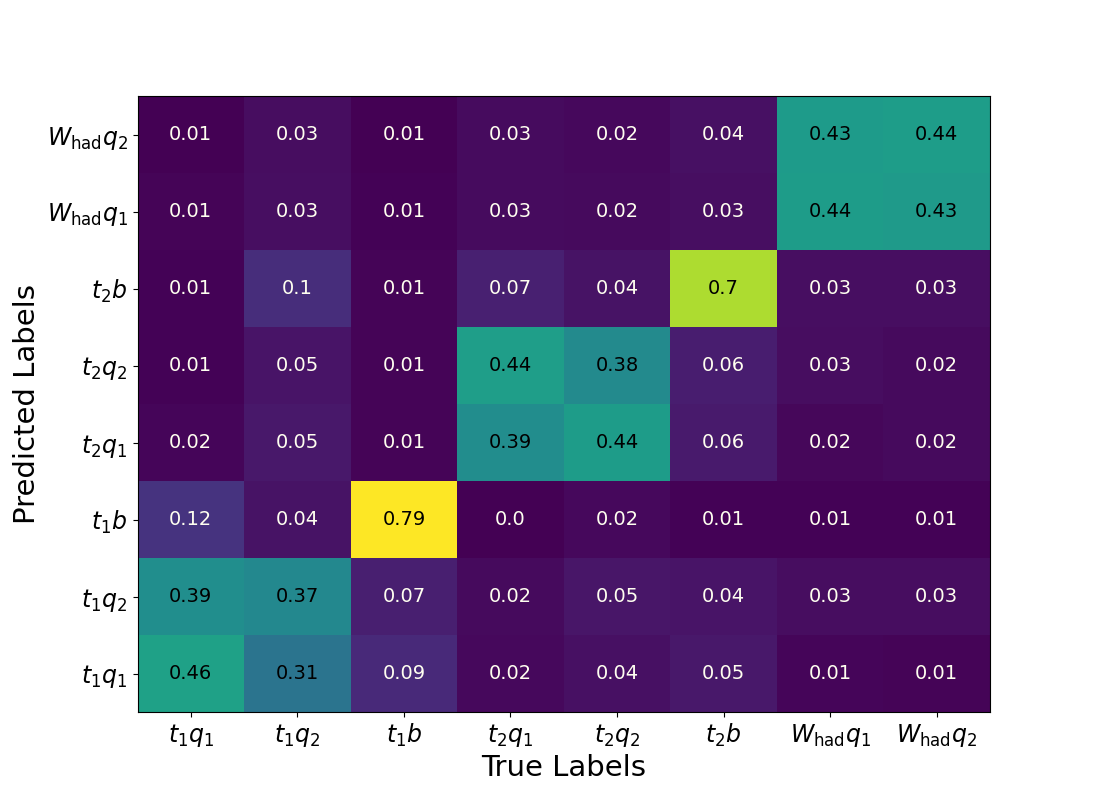
\includegraphics[width=0.48\textwidth]{figures/assignment_matrix/assignment_matrix_a.png}
    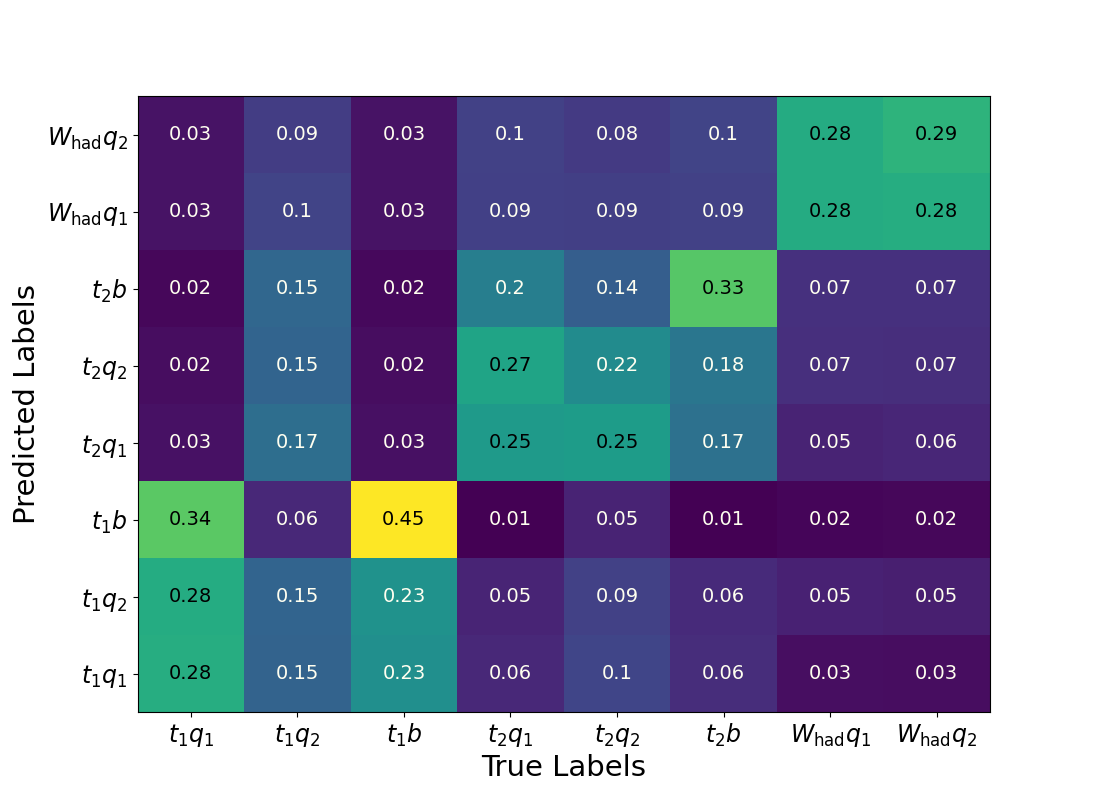
\includegraphics[width=0.48\textwidth]{figures/assignment_matrix/assignment_matrix_1.png}
    \caption{The \spanet prediction confusion matrices showing the predicted and true labels using (left) full events and (right) full and partial events. Each column is normalised to unity.}
    \label{fig:results:spanet:assignment_matrix}
\end{figure}


\subsection*{Probability Output}
The used \spanet implementation outputs a detection and assignment probability for each resonance particle. These probabilities describe \spanets confidence whether the targeted resonance particle exists and whether it is assigned correctly. Additionally, a marginal probability is calculated as the product of assignment and detection probability. These probabilities are visualised in Fig.~\ref{fig:results:spanet:probabilities} for the hadronic $W$-boson from the $H$-boson sub-system. The other output probabilities are listed in Appx.~\ref{appendix:spanet_output_probabilities}.

The detection probability has similar distribution for correct and wrong assignments. However, the distribution has a different shape for events where the targeted resonance particle $W_\text{had}$ does not exist. Hence, the variable can be used to better identify events with a reconstructable hadronic $W$-boson from the $H$-boson decay. 

To differentiate between correct and incorrect predictions, the assignment probability can be used. A particle with high probabilities is more likely to be assigned correctly. Here, the correct and swapped assignments behave very similar which is expected since \spanet treats swapped assignments as correct.

Both metrics further indicate a well-trained network. These metrics are also used in the event selection, to improve the region definition. 

\begin{figure}
    \centering  
    \includegraphics[width=0.48\textwidth]{figures/baptiste/$W_.text{had}$ Detection Probability.png}\hspace{0.02\textwidth}
    \includegraphics[width=0.48\textwidth]{figures/baptiste/$W_.text{had}$ Assignment Probability.png}
    \caption{Normalised distributions of \spanets (left) detection and (right) assignment probabilities for the hadronic $W$-boson from the $H$-boson decay. The events are split into correct, swapped, incorrect and invalid. Invalid events correspond to events where the targeted resonance does not exist. Swapped assignments correspond to swapped assignments within the predefined permutations.}
    \label{fig:results:spanet:probabilities}
\end{figure}

\begin{table}
    \centering
    \caption{Summary of \spanets parton prediction distributions. Both rows contain the relative contribution and absolute number of events for correct, swapped and wrong events. The $t$ quark row contains the average of $t_1$ and $t_2$.}
    \begin{tabular}{c|c|c|c}
        & Correct & Swapped & Wrong \\
        \hline
        $t$ & 8.0\,\% & 7.6\,\% & 84.4\,\%\\
        & 333322 & 31529 & 351634\\
        \hline
        $W_\text{had}$ & 13.8\,\% & 14.1\,\% & 72.1\,\%\\
        & 42729 & 43623 & 222845\\
    \end{tabular}
    \label{tab:results:spanet:probability_yields}
\end{table}

\section{Neutrino Weighting}
\label{sec:results:neutrino_weighting}
As explained in Ch.~\ref{ch:neutrino_weighting}, the deployed \NW algorithm predicts the unknown parameters $\eta_\nu$ and $m_{W^*}$. This is done by calculating the most likely combination of these parameters while using the hadronic $W$-boson from the $H$-boson decay and missing transverse energy $E_T^\text{miss}$ as input. Assuming the decay mode and on-shell mass of the $H$-boson as outlined in Ch.~\ref{ch:event_selection}, the event can be reconstructed using \NW estimations.

%\subsection*{Grid Search}
%Besides using the calculated weight for each event to estimate the most likely unknown parameters, it can also be used in the event selection to reduce backgrounds. Previously, this technique has been estimated to greatly suppress backgrounds in \HWW systems by discarding all events with a neutrino weight $w<0.7$. Using this selection, a theoretical signal purity of 20\% was calculated \cite{neutrino_weighting:adaptation}.

\subsection*{Estimation Heatmaps}
To validate the accuracy of the \NW algorithm, the estimated solutions are compared to the true values of the MC samples. Here, the \NW algorithm uses the truth information as input. Hence, effects due to simulated detector inefficiencies and reconstruction algorithms are ignored in the comparison. 

%\begin{figure}
%    \centering  
%    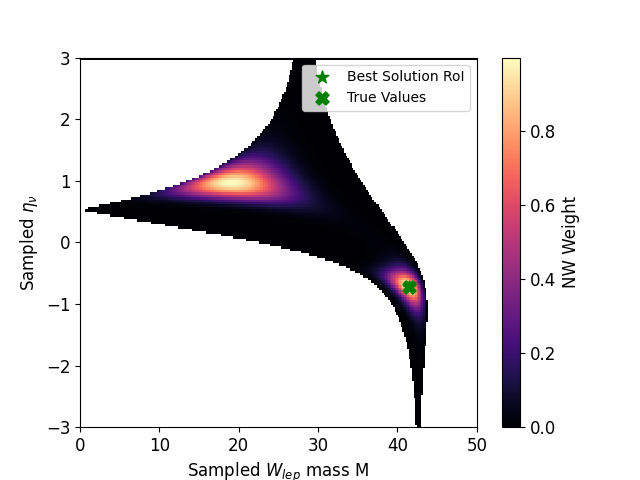
\includegraphics[width=0.7\textwidth]{figures/Neutrino Weighting/cherry_13.png}
%    \caption{Visualisation of the \NW output of a single cherry-picked event. For each sampled combination of $\eta_\nu$ and $m_{W^*}$, calculated weight is shown. The maximum of the weight distribution and the true solutions are marked.}
%    \label{fig:results:neutrino_weighting:cherry}
%\end{figure}

As an additional validation step, the assumed Higgs mass $m_H$ is varied. The MC samples for validation use a true mass of $m_H^\text{MC}=125$\,GeV. The \NW algorithm is tested by assuming the correct mass of $m_H=m_H^\text{MC}$ and a slightly off-set mass $m_H=125.2$\,GeV. Fig.~\ref{FIG:neutrino_weighting:validation_higgs_mass} shows the difference of the estimated values of $\eta_\nu$ and $m_W$ for both assumptions. The heatmaps clearly show the sensibility of the algorithm in respect to the assumed $H$-boson mass. Furthermore, for a correct assumption $m_H=m_H^\text{MC}$, the distribution peaks around ($\nu_\eta=0$, $m_{W^*}=0$\,GeV) as expected. Using a different $H$-boson mass significantly changes the estimated mass its decay particle $W_\text{lep}$. Hence, when using $m_H=125.20$\,GeV the estimated mass $m_W$ is increased by around 200\,MeV in respect to the true value due to kinematic conservation laws. This sensitivity is expected to introduce a systematic uncertainty in regards to the assumed $m_H$ which should be studied. However, this thesis does not include the analysis of systematic uncertainties. When using data, the $m_H$ assumption needs to be changed to $m_H=125.09$\,GeV as stated in Ch.~\ref{ch:neutrino_weighting}.

\begin{figure}
    \centering
    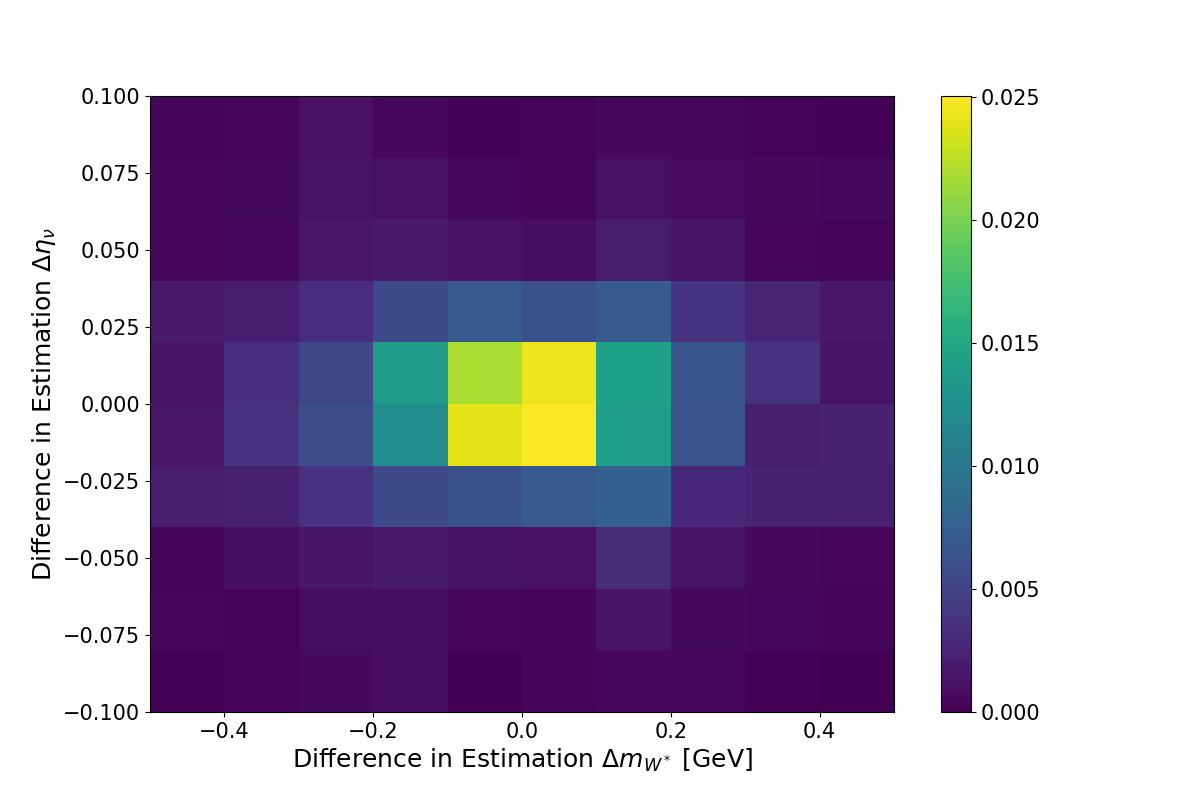
\includegraphics[width=0.49\textwidth]{figures/Neutrino Weighting/truth_2d_delta_mw_delta_nueta.png}\hspace{0.01\textwidth}
    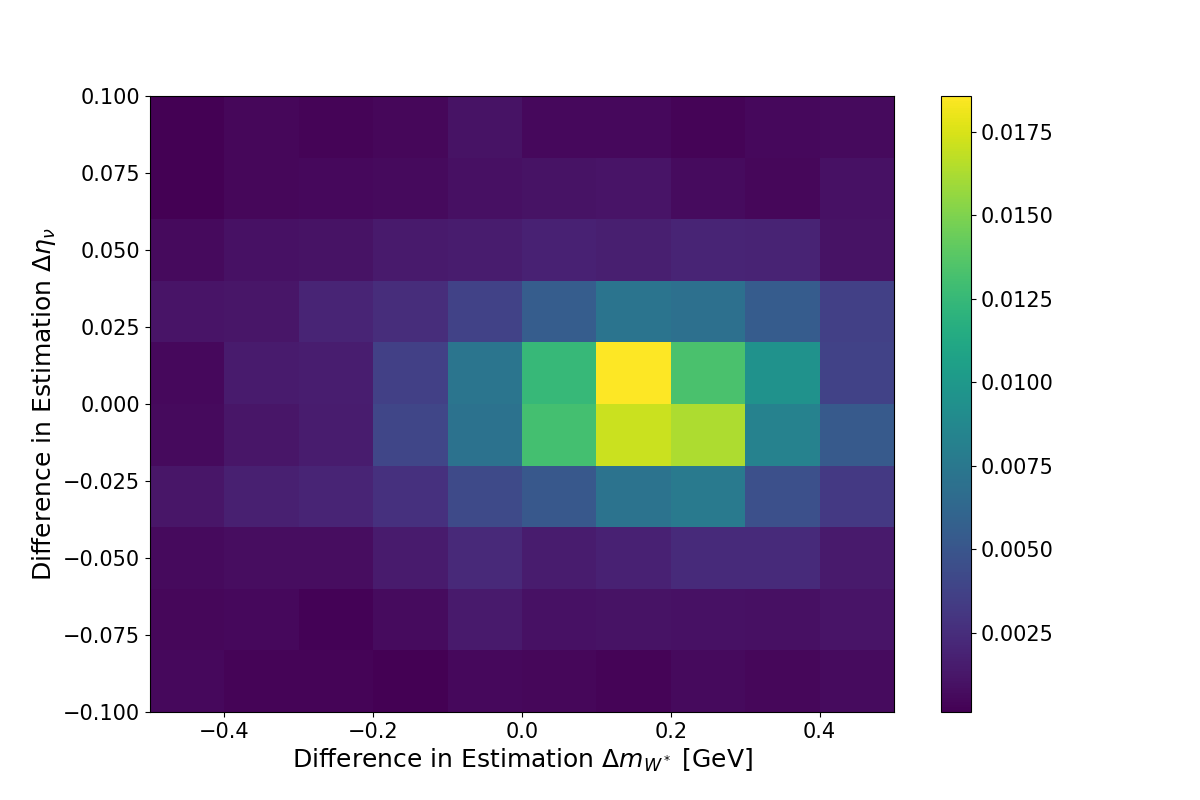
\includegraphics[width=0.49\textwidth]{figures/Neutrino Weighting/truth_alt_2d_delta_mw_delta_nueta.png}
    \caption{Comparison of two heatmaps showing the difference between the estimated and true values. The two heatmaps use (left) the correct $m_H=m_H^\text{MC}$ and (right) the off-set $m_H=125.20$\,GeV.}
    \label{FIG:neutrino_weighting:validation_higgs_mass}
\end{figure}

Furthermore, in Fig.~\ref{FIG:neutrino_weighting:true_and_reco} the same distribution is shown. Here, the $H$-boson mass is not varied, but the input uses the reconstructed information, including simulated detector effects. Again, the predictions are centred around ($\nu_\eta=0$,$m_{W^*}=0$\,GeV). However, when using reconstructed information as input, the \NW estimations deviate stronger from the true values. These inaccuracies are expected due to less accurate inputs. Hence, the dependence on the jet and kinematic accuracies is expected to be an important systematic that should be studied. 

\begin{figure}
    \centering
    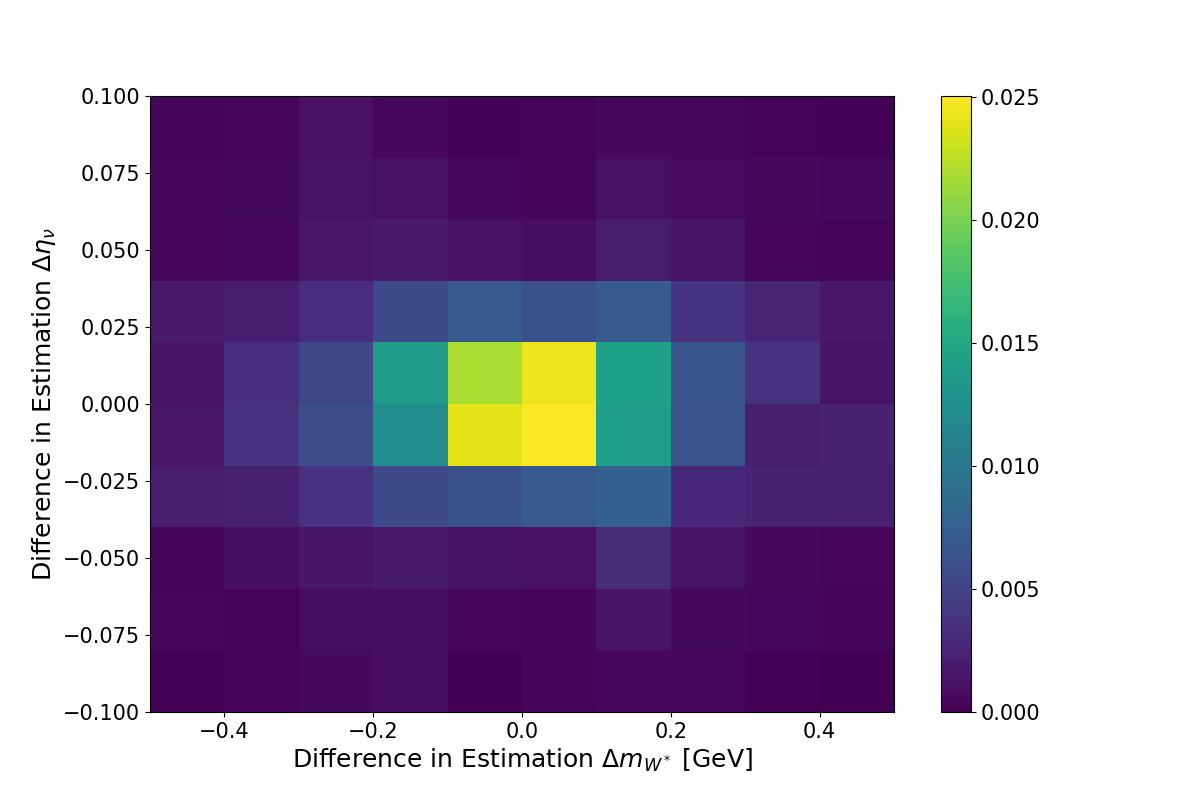
\includegraphics[width=0.49\textwidth]{figures/Neutrino Weighting/truth_2d_delta_mw_delta_nueta.png}\hspace{0.01\textwidth}
    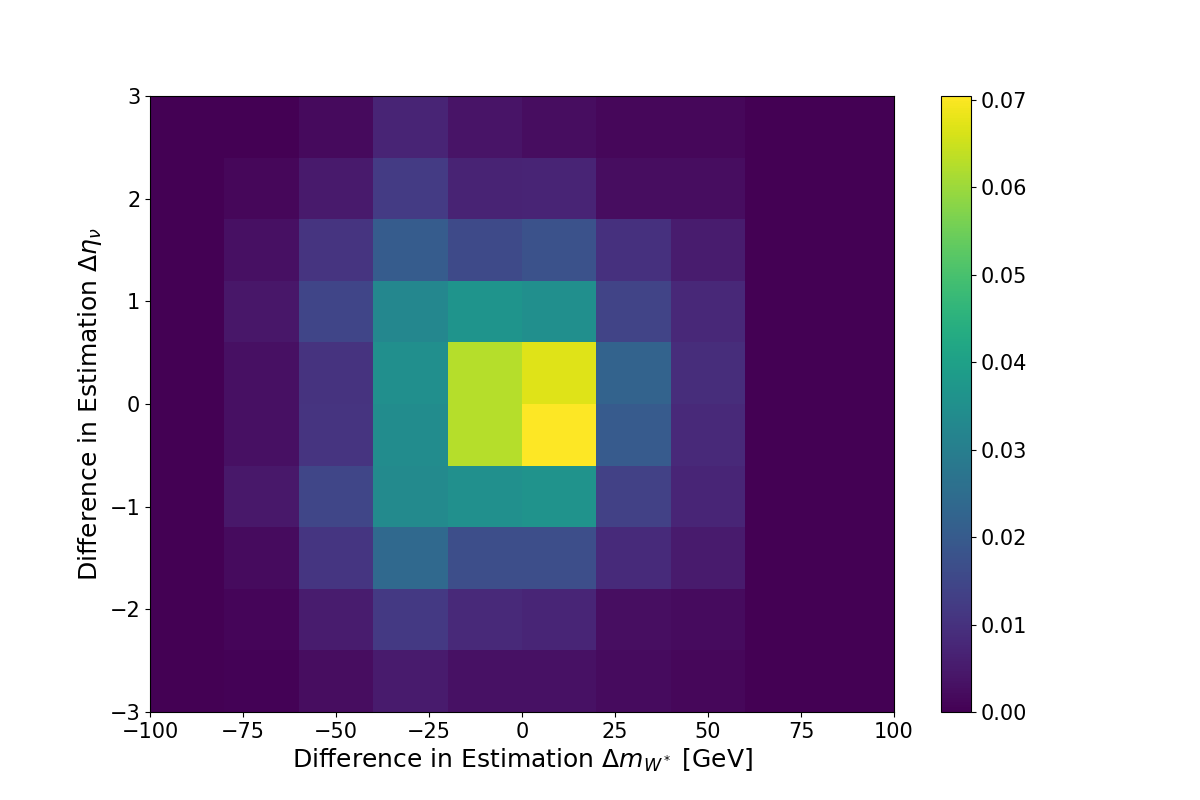
\includegraphics[width=0.49\textwidth]{figures/Neutrino Weighting/reco_2d_delta_mw_delta_nueta.png}
    \caption{Comparison showing the \NW output difference when using (left) true information and (right) reconstructed information as input. Note the different scales.}
    \label{FIG:neutrino_weighting:true_and_reco}
\end{figure}

\subsection*{Performance}
To evaluate the \NW algorithm, different setups have been tested. Each setup differs in its input variables, grid size and use of the optimisations which are explained in Sec.~\ref{sec:neutrino_weighting:optimisation}. The results are listed in Tab.~\ref{tab:results:neutrino_weighting:performance}. To quantify the performance, three metrics are calculated. 

The average signal weight $\bar{w}_\text{signal}$ from the \NW algorithm is an indicator, how good the reconstruction is. It is the arithmetic mean of all calculated weights of all events with at least one solution. Values close to 1 correlate to estimations matching the observed values closely. Lower values correspond to estimations of lower quality. The signal reconstruction efficiency $\epsilon_\text{signal}$ equals the number of signal events containing at least one solution divided by the total number of signal events. Higher efficiencies mean that the \NW algorithm finds solutions for signal events more often. Hence, more \ttHWW events become reconstructable, regardless of the solution quality. The reconstruction purity $p_\text{signal}$ is the ratio of reconstructed semileptonic \ttHWW events to all reconstructed events. A high purity means less background events have a \NW solution, regardless of their quality. 

All metrics should be optimised simultaneously to ensure sufficient numbers of signal events with high quality solutions. The table shows that the algorithm is able to achieve a 100\,\% purity when using the truth values as input. While this result is unrealistic, it further validates the algorithm's estimations. As expected, the average weight and efficiency is the highest when using the exact truth values as input.

Three more test were conducted when using the reconstructed input while ignoring the \spanet prediction. Instead, the correct assignment is used. These three test give a more realistic insight into how well the algorithm works independently of the \spanet performance. All three metrics decrease overall which is expected due to the less accurate input. When increasing the grid granularity, the average weight and purity increase slightly. However, this effect can also be achieved by using the aforementioned optimisations. The increase in $\bar{w}_\text{signal}$ originates from the introduced regions of interest while the changes in the efficiency and purity originate from the $H$-boson mass smearing. The comparison shows that a 100x100 grid size including the optimisations is sufficient. Additionally, the optimised setup uses fewer computing resources than using bigger grid sizes.

Lastly, the final setup is evaluated which uses the 100x100 grid with optimisation but also uses \spanets predictions. Due to the \spanet performance, some jets are incorrectly matched. The resulting incorrect parton reconstruction leads to more background events being reconstructable and thus, the purity decreasing to 45.3\,\%. Moreover, more signal events are now reconstructable which can be seen in the increase of $\epsilon_\text{signal}$. This is expected to originate from signal events that do not fulfil the event assumptions. With correct assignments, the \NW algorithm does not find a solution. When some partons are assigned incorrectly, the reconstructed properties vary. Thus, the incorrect event properties can yield a solution event when the on-shell or decay assumption is not fulfilled. Overall, the reconstruction quality is slightly seen by the decreased average weight.

\begin{table}
    \centering
    \caption{Summary of the \NW performance on all events using different setups. Each setup is evaluated for the \ttHWW signal by comparing the average weight $\bar{w}$, the reconstruction efficiency $\epsilon$ and the reconstruction purity $p$. The highlighted setup is used.}
    \begin{tabular}{l|ccc}
        Setup & $\bar{w}_\text{signal}$ & $\epsilon_\text{signal}$ & $p_\text{signal}$\\
        \hline
        truth input (200x200) & 0.610 & 92.2\,\% & 100\,\% \\[2mm]
        reconstructed input (100x100) & 0.226 & 9.3\,\% & 77.0\,\% \\
        reconstructed input (200x200) & 0.254 & 9.3\,\% & 77.2\,\% \\
        reconstructed input (100x100) + optimisations & 0.252 & 9.4\,\% & 76.8\,\% \\[2mm]
        \rowcolor{highlighter!40}
        \spanet input (100x100) + optimisations & 0.231 & 25.6\,\% & 45.3\,\% \\  
    \end{tabular}
    \label{tab:results:neutrino_weighting:performance}
\end{table}


\section{Data}
\label{results:data}
This section contains the analysis of the combined \runi and \runii{} \atlas dataset using the final \spanet model and the optimised \NW algorithm.

\subsection*{Signal and Control Regions}
The region yield is compared when using data instead of the MC samples. The results for data can be seen in Tab.~\ref{tab:data:regions}. Compared to the results in Tab.~\ref{tab:event_selection:regions}, the relative yield of each region differs by less than 2\,\%. When taking the statistical uncertainties into account, he $SR$ contributions are within a $1\sigma$-interval. For both $CR$s, the statistical uncertainties become relatively small due to their high amount of events per region. Hence, an investigation into systematic uncertainties would be beneficial to evaluate high-statistic regions. In particular, systematic uncertainties regarding the variables used in the region definition and the theoretical modelling uncertainties for \ttbar and \ttHbb are expected to be important contributions.

\begin{table}
    \centering
    \caption{Summary of the event yields using the combined \atlas dataset of \runi and \runii. The region definition is outlined in Sec.~\ref{sec:event_selection:region_definition}.}
    \begin{tabular}{l|c|c|c}
        & $SR$ & $CR_{t\bar{t}}$ & $CR_{H\rightarrow bb}$ \\
        \hline
        Event Count & $67\pm8$ & $2501793\pm1582$ & $752538\pm868$\\
        Relative Yield & $(0.0021\pm0.0003)\,\%$ & $(76.87\pm0.05)\,\%$ & $(23.12\pm0.03)\,\%$\\
    \end{tabular}
    \label{tab:data:regions}
\end{table}


\subsection*{Comparison}
Several variables have been investigated to further compare the \atlas dataset to the MC simulation. The event distributions of several selected variables are shown in Fig.~\ref{fig:data:comparison}. All other investigated variables show similar behaviour. Their distributions can be found in Appx.~\ref{appendix:mc_data_comparisons}.

The MC samples and dataset show similar behaviour for measured quantities and derived variables alike. The normalised event distributions have almost identical shapes and their respective values are mostly within a $3\sigma$-interval of each other although only statistical uncertainties are included. Due to the high statistics available, some bins contain very small uncertainties. 

The most notable difference is seen in the missing transverse energy $E_T^\text{miss}$ and the $b$-jet multiplicity. The MC sample contains higher contributions of events with $E_T^\text{miss}>70\,$GeV and thus, the shape is slightly shifted towards higher $E_T^\text{miss}$. Moreover, the $b$-jet multiplicity shows a deficit of 5-20\,\% for events with $\geq3$ $b$-jets when comparing the MC sample to the dataset.

However, the mentioned deviations as well as others exceeding a $3\sigma$-interval are expected to be resolved when including their respective systematic uncertainties such as $b$-tagging efficiencies or $E_T^\text{miss}$ resolution. For the derived quantities such as \spanets probabilities and \NW output, systematic uncertainties related to their input variables should resolve significant deviations. 

\begin{figure}
    \centering
    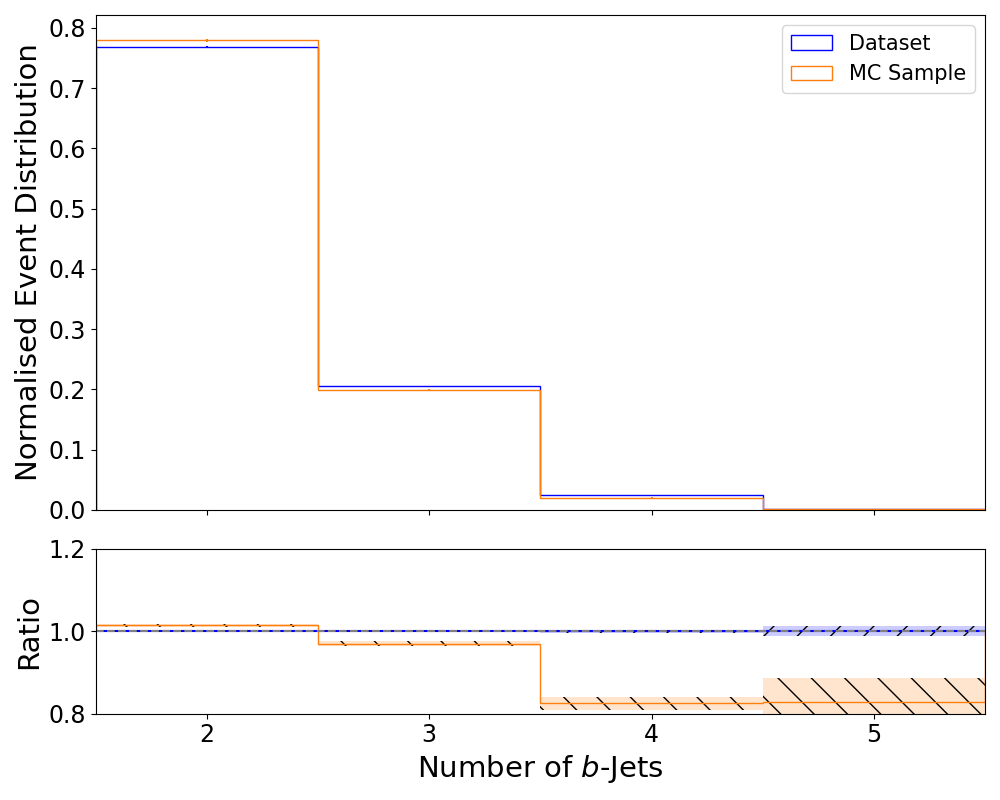
\includegraphics[width=0.49\textwidth]{figures/comparison/number_of_bjets.png}\hspace{0.01\textwidth}
    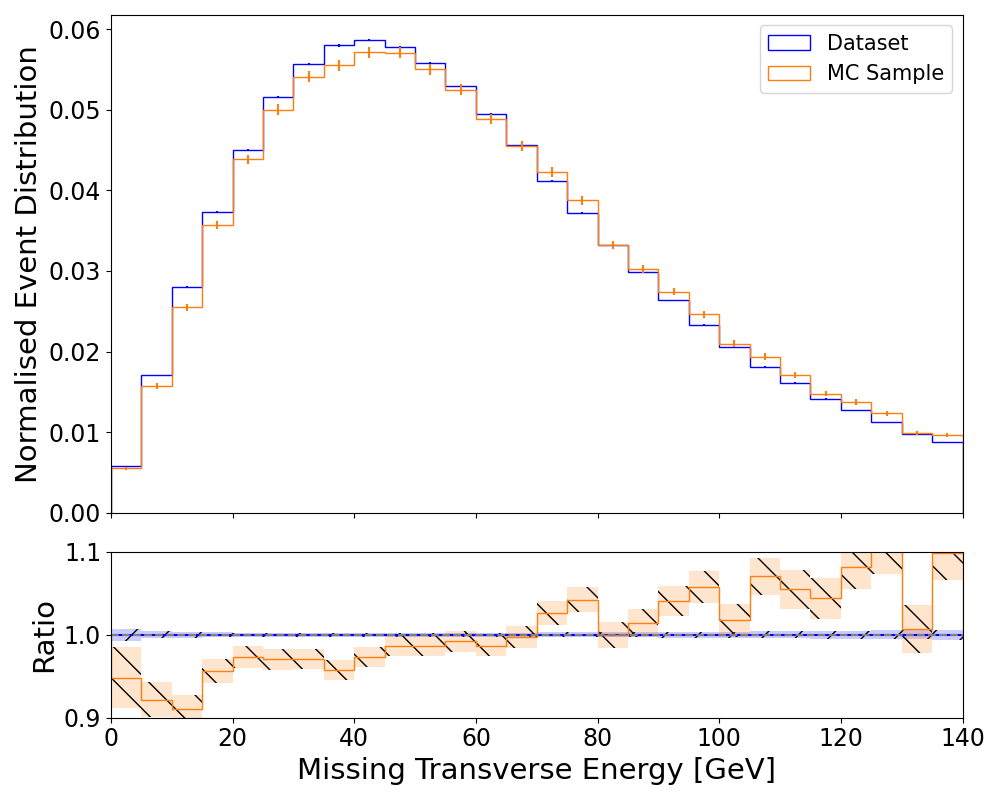
\includegraphics[width=0.49\textwidth]{figures/comparison/reco_met_value.png}

    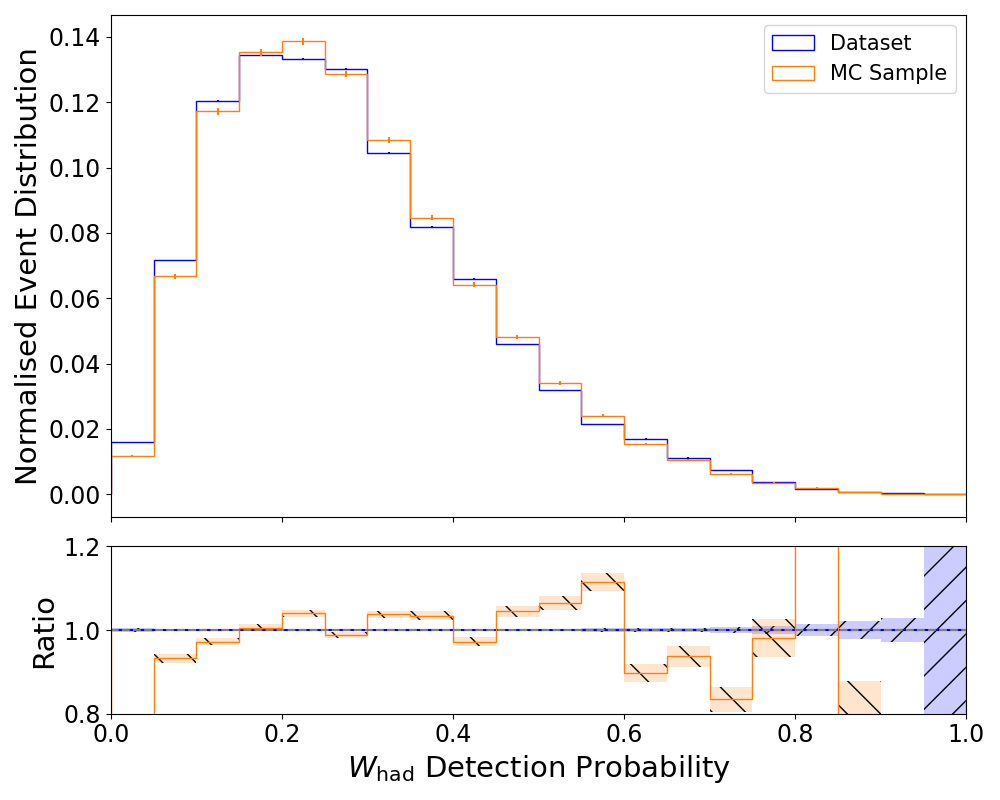
\includegraphics[width=0.49\textwidth]{figures/comparison/spanet_HW_detection_probability.png}\hspace{0.01\textwidth}
    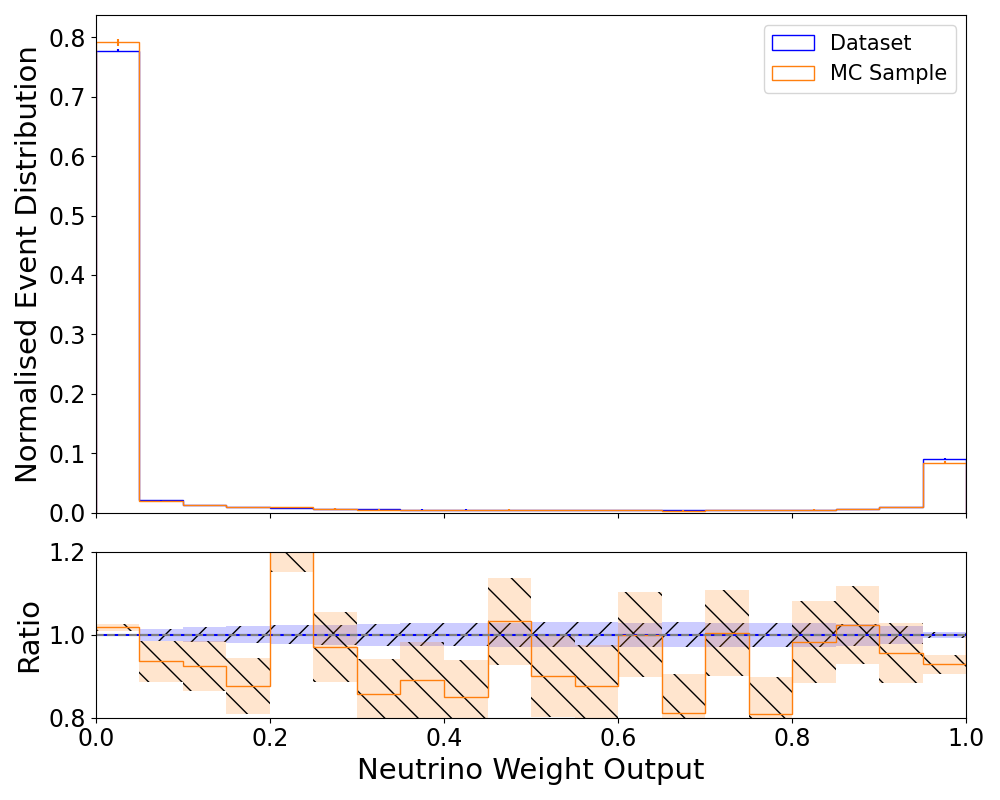
\includegraphics[width=0.49\textwidth]{figures/comparison/NW_weight.png}
    \caption{Comparison of the normalised MC and data event distributions for selected variables. These include the (top left) total jet multiplicity, (top right) missing transverse energy, (bottom left) \spanets $W_\text{had}$ detection probability and (bottom right) \NW output. Only statistical uncertainties are shown.}
    \label{fig:data:comparison}
\end{figure}


\chapter{Discussion}
\label{ch:outlook}
To conclude this thesis, a summary of the main results is given in Sec.~\ref{sec:discussion:summary}. This section will reiterate the main measurements with respect to the main goal of this analysis. Lastly, inspiration for future steps of this analysis are explained in Sec.~\ref{sec:discussion:future}.

% - Compare to Steffens Paper, Numbers for certrain event types (e.g. ttbar, ttH->WW->qqlv, ...)
\section{Summary}
\label{sec:discussion:summary}
As explained in Sec.~\ref{sec:theory:tthww}, the targeted semileptonic \ttHWW event topology is difficult to measure due to its rarity. The theoretical calculation expects over 10000 background events per signal event. This corresponds to a signal purity of less than 0.01\,\%. Using \spanet and \NW to analyse and separate the simulated events led to the region definition in Sec.~\ref{sec:event_selection:region_definition}. For the signal region $SR$ the purity of \ttHWW events reaches 0.44\,\%. However, the main \ttbar background still dominates the $SR$ region with over 99\,\% contribution which is caused by the significant higher cross-section of this process. The \ttHbb background was efficiently separated by simply selecting an excess in $b$-jets. This singular selection separated 75.0\,\% of the \ttHbb background. This sensitivity study shows that the outputs of the deployed techniques can be used to increase the signal sensitivity significantly, but the event channel remains difficult to separate from background.

This study further tested and evaluated the adaptation of \spanet and \NW for event studies. It is shown that a properly trained neural network can efficiently assign jets to expected parton as demonstrated in Sec.~\ref{sec:results:spanet}. Simultaneously, \spanet produces output probabilities which can be used for the event definition. Furthermore, as shown in Sec.~\ref{sec:results:neutrino_weighting}, the \NW algorithm can be successfully adapted to events with only one neutrino in the final state. When using a truth-based input, the algorithm is able to reconstruct the unknown parameters with <1\,\% deviation. While this is unrealistic, this demonstrates its ability to precisely estimate unknown kinematics when using sufficiently accurate input. Moreover, the deployed optimisations as explained in Sec.~\ref{sec:neutrino_weighting:optimisation} are efficient additions to the \NW. They omit the need of additional grid points which reduces the needed computing resources. Additionally, the event acceptance is increased due to the smearing of assumed $H$-boson mass. However, the results also show that the algorithm is highly dependent on the input accuracy. Therefore, the \NW is only viable when the analysis uses precise measurements and confident jet assignments.

For the comparison of the \atlas dataset of \runi and \runii combined to the MC samples, the regions and several variables were investigated. The results in Sec.~\ref{results:data} show similar behaviour with little differences in the overall shape. The normalised values of each distribution mostly match within a $3\sigma$-interval when considering statistical uncertainties only. The remaining deviations are expected to resolve when including the respective systematic uncertainties as explained. Especially the control region comparison will benefit greatly from systematic uncertainties due to the very high statistics in both $CR$. In conclusion, this study substantiates that the MC samples for \atlas dataset is well modelled and hence, can be used reliable when training neural networks and evaluating algorithms.


\section{Future Aspects}
\label{sec:discussion:future}
This section outlines potential tasks for the future. While this study provides insights into the \ttHWW event separation, there remain opportunities for refinement. These potential future tasks are explained briefly. However, due to time constraints these optimisations exceeded the scope of this work.

\subsection*{Include Systematic Uncertainties}
This study only includes statistical uncertainties for the final results. Hence, systematic uncertainties due to detector calibrations, theoretical models, luminosity and other effects are not included. In the future, this analysis should be complemented by introducing these systematic uncertainties. 

Especially the \NW performance evaluation would benefit studying the systematic uncertainties introduced by the used input as explained in Sec.~\ref{sec:results:neutrino_weighting}. Varying the systematic uncertainties would result in a more detailed understanding of the algorithm and its sensitivity in respect to the input.

Combining systematic and statistical uncertainties will yield more realistic uncertainties for the measurements. Moreover, varying the systematic uncertainties would show the sensitivity of the measurements with respect to the investigated uncertainties. Hence, the reduction of the most sensitive uncertainties should then be prioritised to improve the results of this study. 

\subsection*{Further Optimisation}
While this study includes several technical optimisations, additional improvements should be tested in the future. 

As seen in this study, \spanets prediction accuracy is limited by the correct \ttbar assignment. Hence, training the neural network to assign these jets correctly should improve the overall performance of this analysis. This could be done, by initially training \spanet only on \ttbar events and then fine-tuning the parameters for \ttHWWlvqq events. Since \ttbar events are the main background in this analysis, this could also help to increase the signal purity in the event selection. 

The \NW algorithm also includes some optimisations such as the regions of interest and $H$-boson mass smearing. As an additional improvement, changing the $\eta_\nu$ sampling to an adaptive approach could improve algorithm by reducing the number of needed samples. The expected $\eta_\nu$ is depend on the overall event energy, making certain regions more likely to contain a solution.


\bibliography{datenbank} 

\appendix
\chapter{Additional SPA-Net Output Probabilities}
\label{appendix:spanet_output_probabilities}
\begin{figure}[H]
    \centering  
    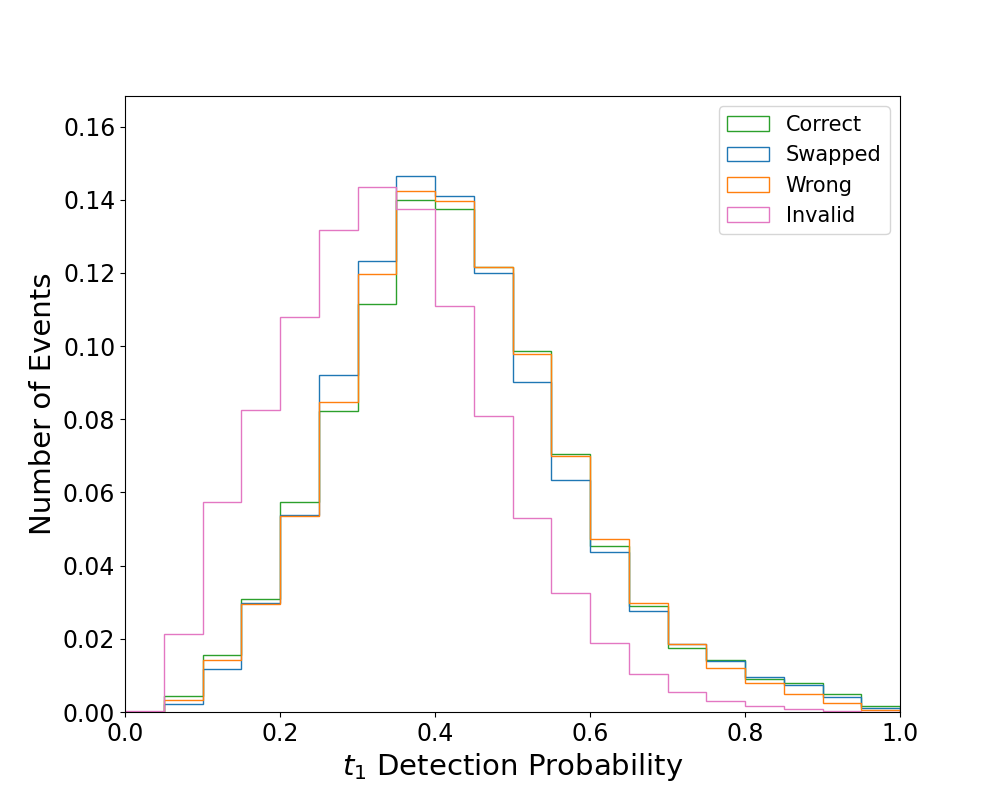
\includegraphics[width=0.49\textwidth]{figures/baptiste/$t_1$ Detection Probability.png}\hfill
    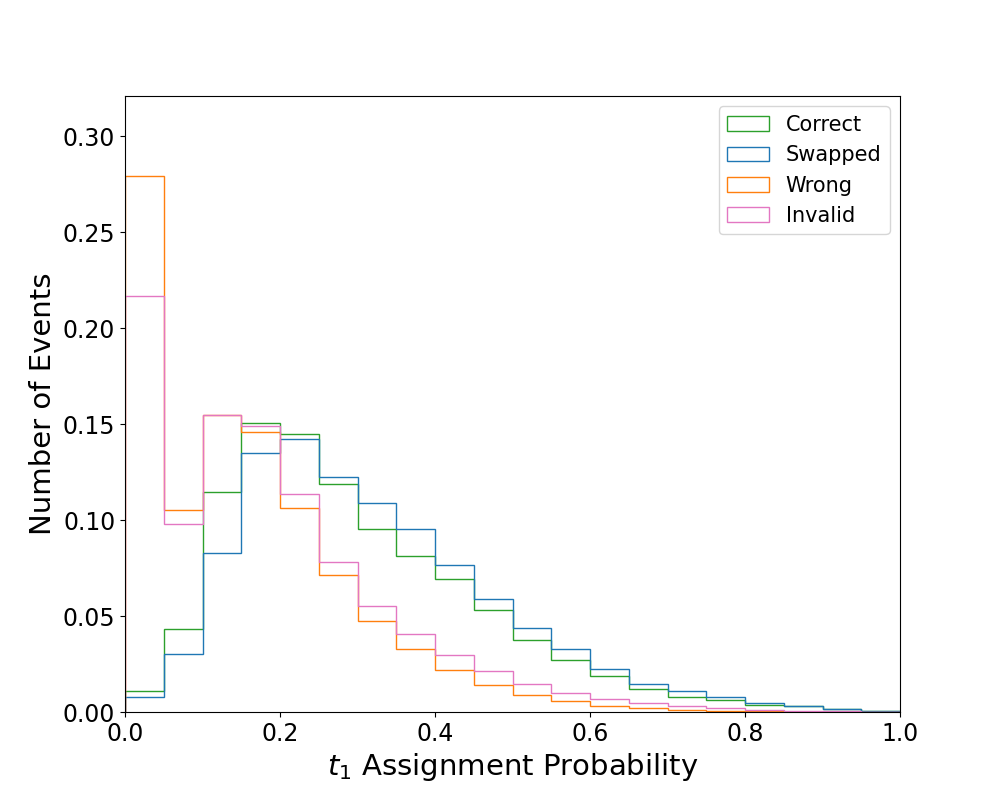
\includegraphics[width=0.49\textwidth]{figures/baptiste/$t_1$ Assignment Probability.png}

    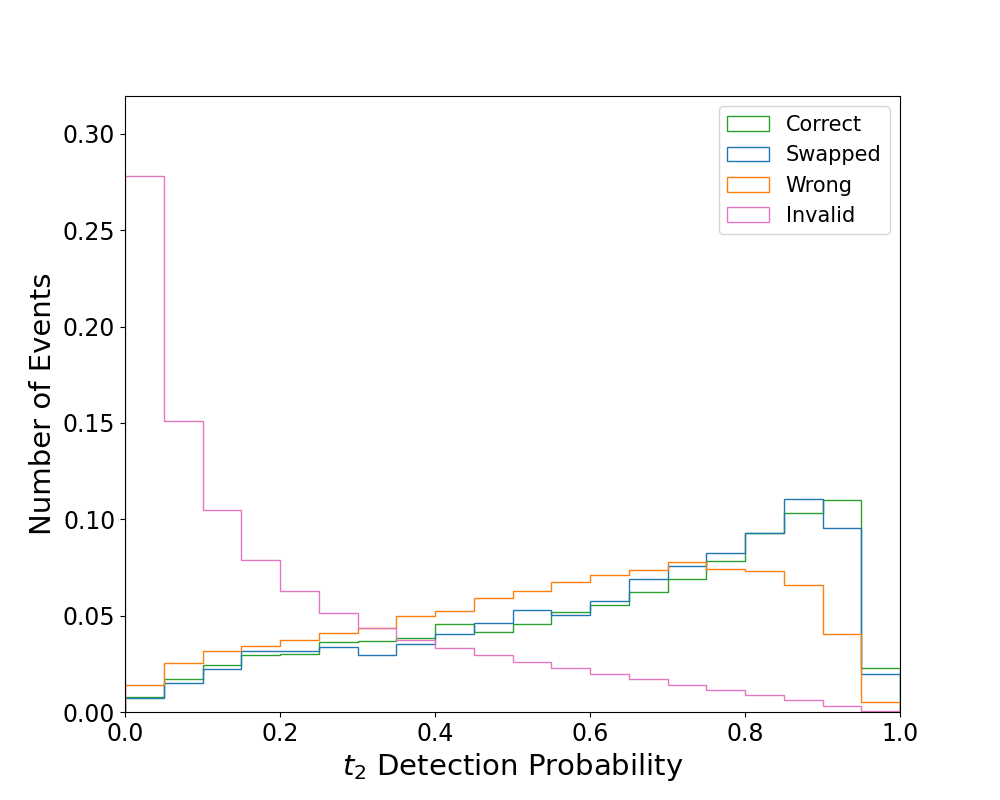
\includegraphics[width=0.49\textwidth]{figures/baptiste/$t_2$ Detection Probability.png}\hfill
    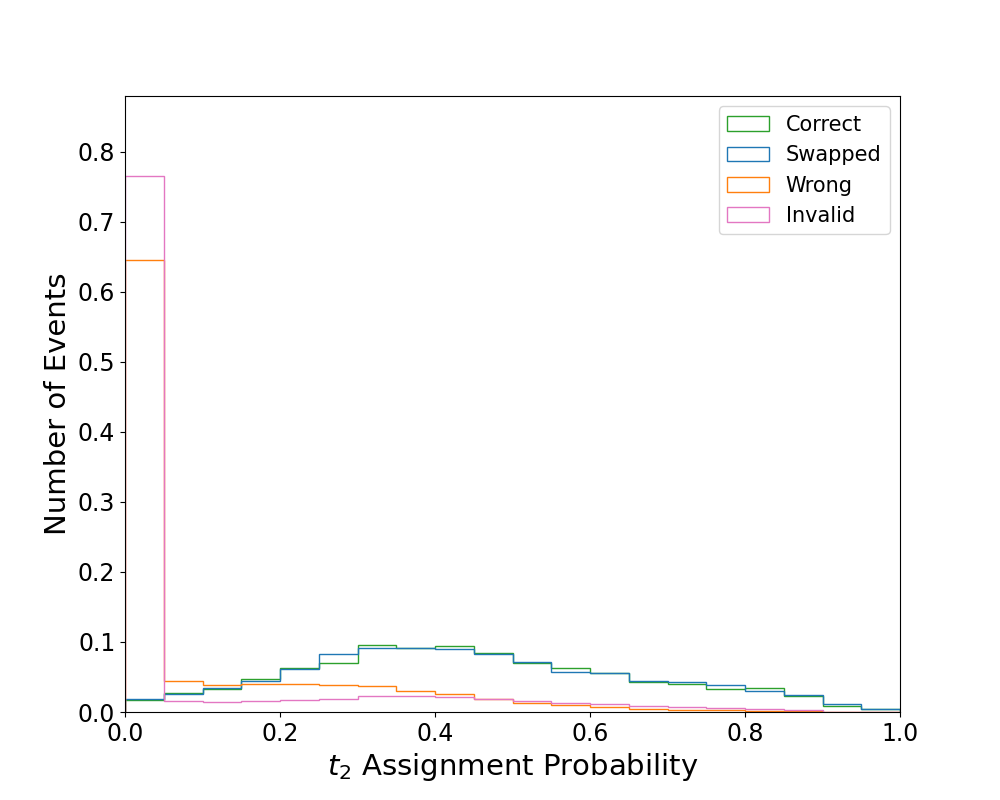
\includegraphics[width=0.49\textwidth]{figures/baptiste/$t_2$ Assignment Probability.png}

    \includegraphics[width=0.49\textwidth]{figures/baptiste/$W_.text{had}$ Detection Probability.png}\hfill
    \includegraphics[width=0.49\textwidth]{figures/baptiste/$W_.text{had}$ Assignment Probability.png}
\end{figure}

\chapter{Additional Comparisons of Atlas Dataset and MC Samples}
\label{appendix:mc_data_comparisons}
\begin{figure}[H]
    \centering
    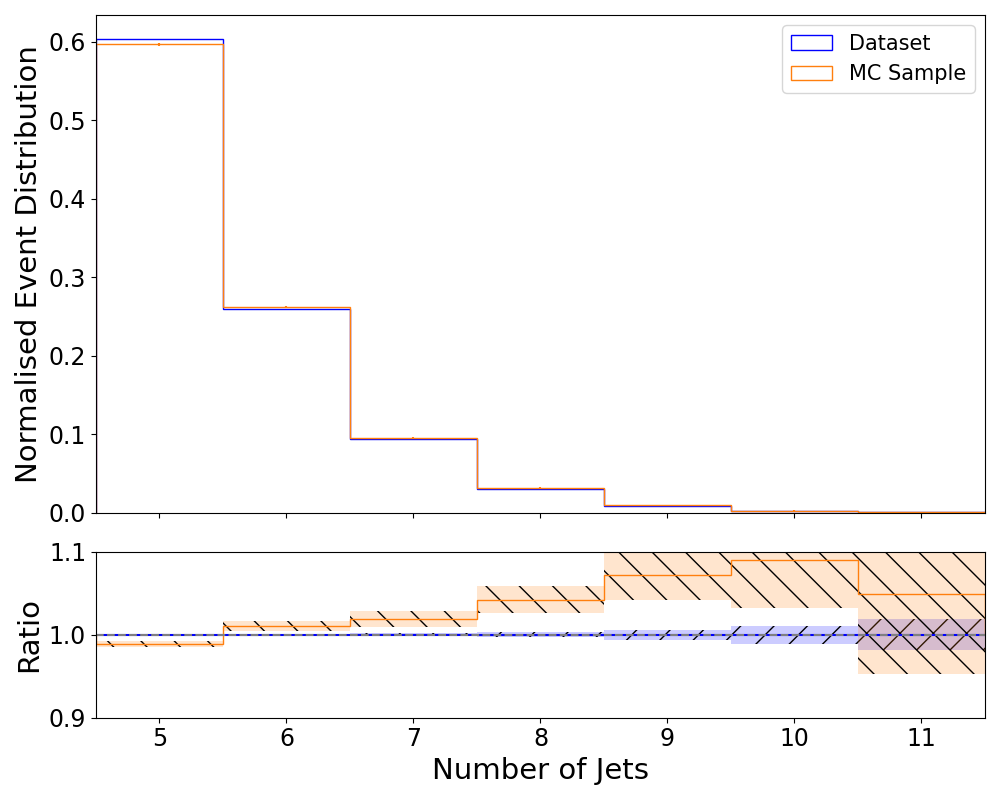
\includegraphics[width=0.49\textwidth]{figures/comparison/number_of_jets.png}\hspace{0.01\textwidth}
    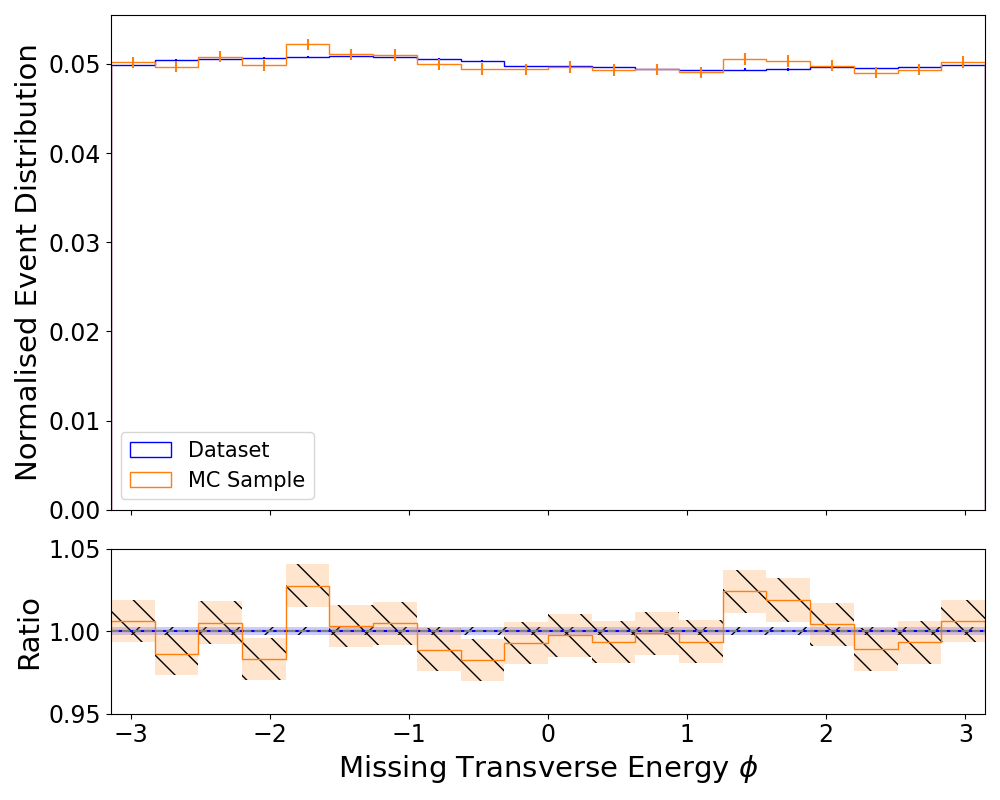
\includegraphics[width=0.49\textwidth]{figures/comparison/reco_met_phi.png}

    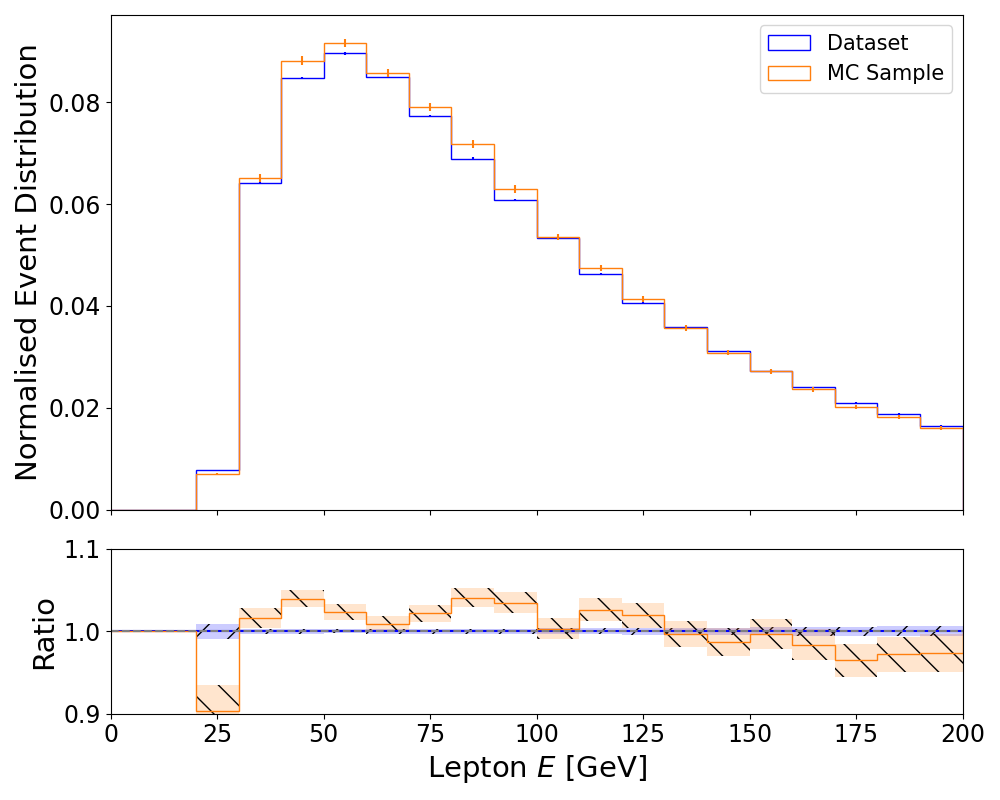
\includegraphics[width=0.49\textwidth]{figures/comparison/reco_lepton_e.png}\hspace{0.01\textwidth}
    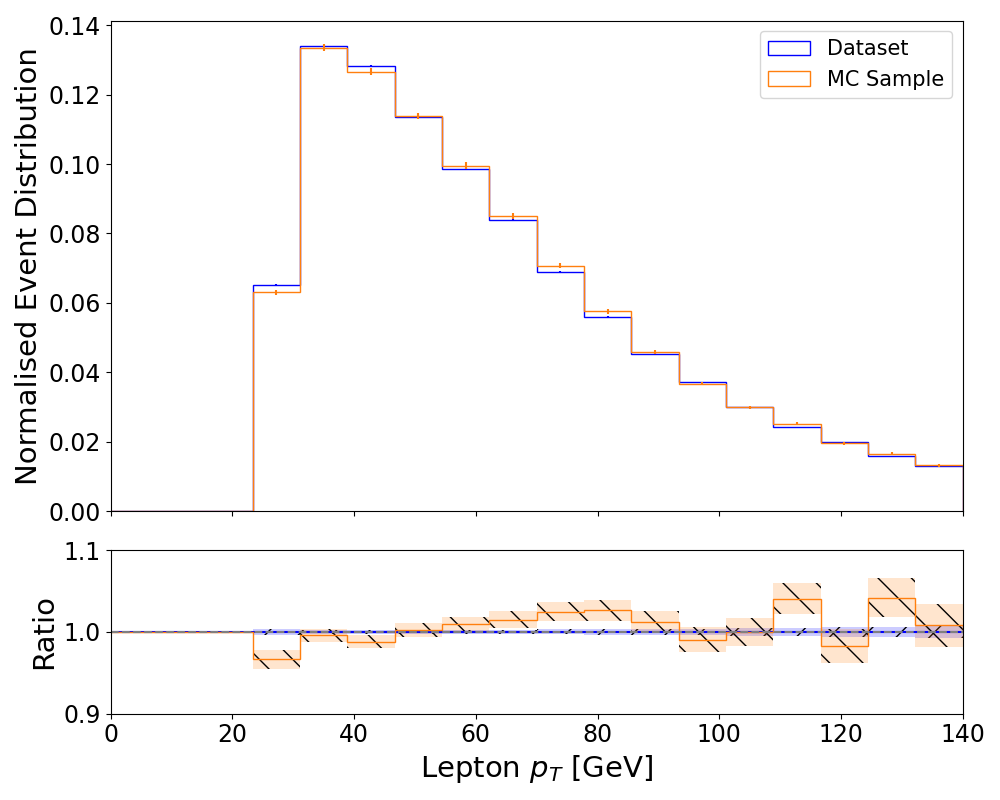
\includegraphics[width=0.49\textwidth]{figures/comparison/reco_lepton_pt.png}

    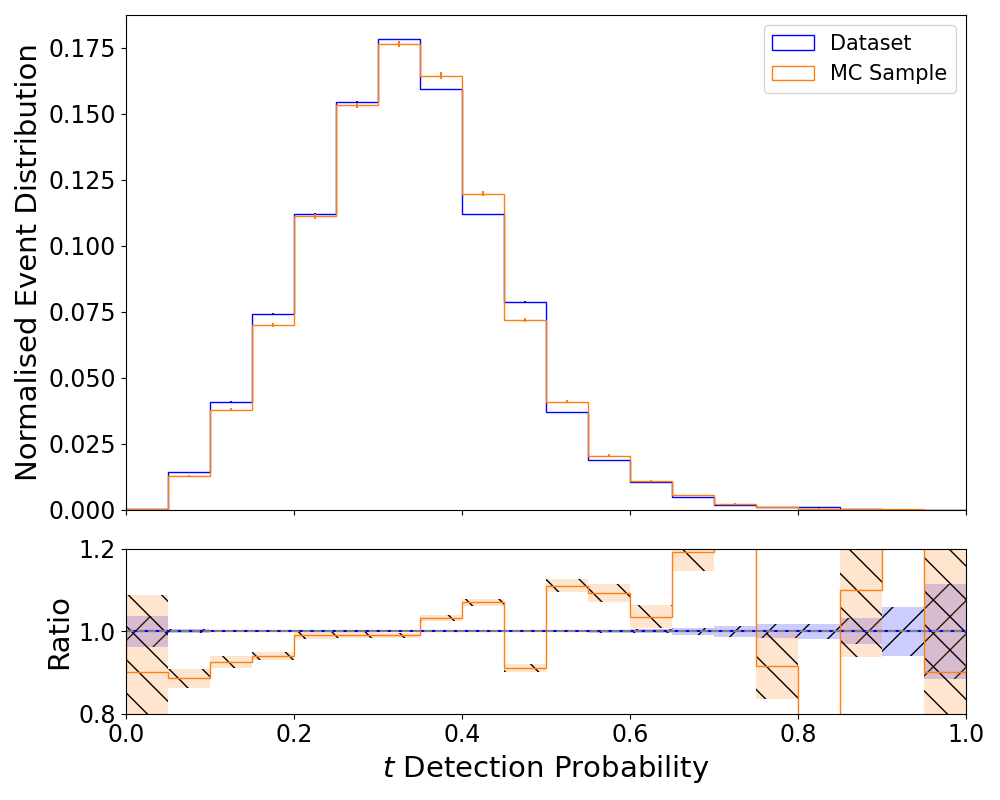
\includegraphics[width=0.49\textwidth]{figures/comparison/spanet_t1_detection_probability.png}\hspace{0.01\textwidth}
    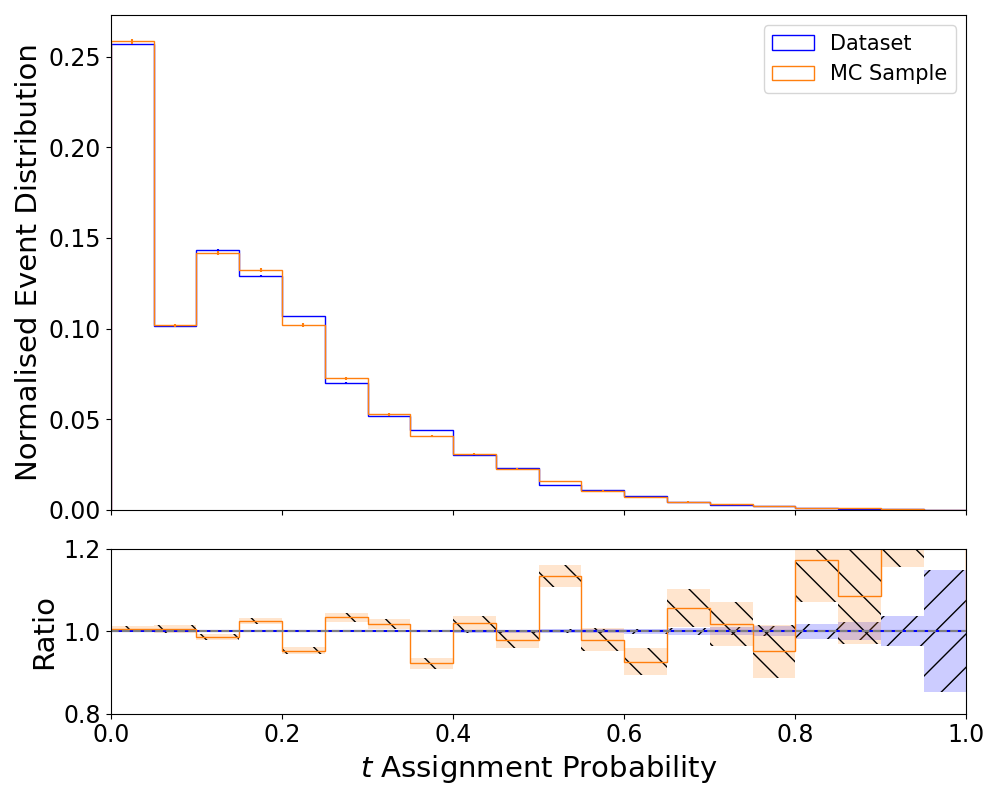
\includegraphics[width=0.49\textwidth]{figures/comparison/spanet_t1_assignment_probability.png}
    \label{fig:data:comparison}
\end{figure}

% obligatory declaration
\chapter*{Declaration}
\vfill
\begin{otherlanguage}{ngerman}
    \Declaration
    
    \begin{figure}
        \centering
        \vspace*{-37mm}    
        \hspace{20mm}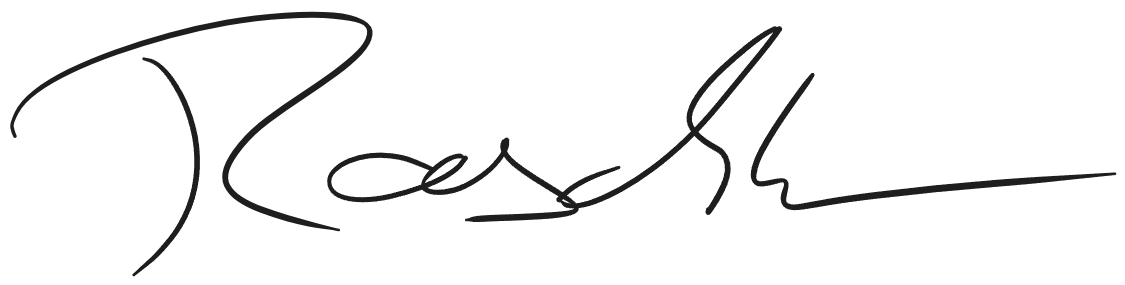
\includegraphics[width=.6\textwidth]{figures/signature.png}	
    \end{figure}
\end{otherlanguage}

    
\end{document}
